%!TEX root = ../csuthesis_main.tex
% 论文正文是主体，主体部分应从另页右页开始，每一章应另起页。一般由序号标题、文字叙述、图、表格和公式等五个部分构成。
\section{绪论}
\subsection{研究背景与意义}

随着人工智能与计算机视觉技术的飞速发展，人体姿态估计（Human Pose Estimation, HPE）作为连接数字世界与物理世界的关键纽带，已在众多领域展现出巨大的应用价值。该技术旨在从图像或视频中定位人体关键点（如肩、肘、腕、膝等）并构建骨架结构，广泛应用于人机交互、虚拟现实/增强现实（VR/AR）、智慧医疗康复、体育动作分析以及智能安防监控等场景。特别是在医疗康复领域，通过精确捕捉患者的运动轨迹，系统能够量化评估肢体功能，辅助医生制定个性化的治疗方案。
如图~\ref{fig:hci_scenario}所示，机器人与人交互场景通常同时存在多目标与遮挡，因而对多人三维姿态的实时感知提出更高要求。

\begin{figure}[htbp]
  \centering
  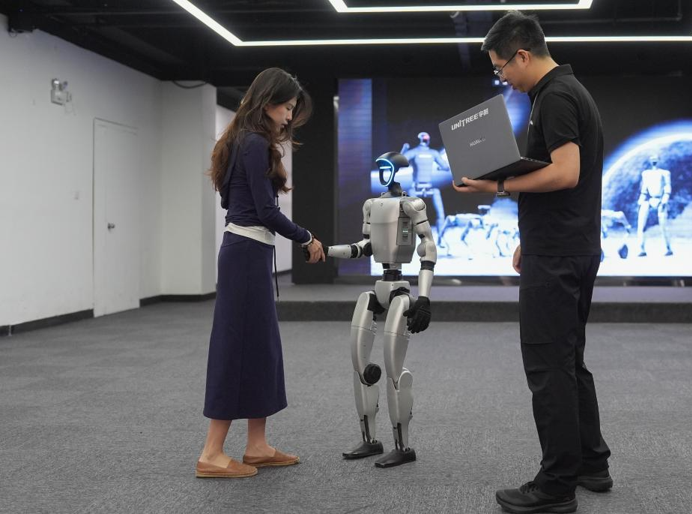
\includegraphics[width=0.9\textwidth]{images/Human_computer_interaction_scenario.png}
  \caption{机器人与人交互场景下多人三维人体姿态感知的重要性示意}
  \label{fig:hci_scenario}
\end{figure}

尽管基于深度学习的二维（2D）人体姿态估计技术已趋于成熟，但其仅能提供平面位置信息，缺乏深度维度，难以完整反映人体在三维空间中的真实姿态与运动细节，限制了其在复杂交互场景下的应用潜力。三维（3D）人体姿态估计能够恢复人体关节的空间坐标，提供更丰富的运动学信息。然而，直接从单目图像恢复3D姿态本质上是一个不适定问题（Ill-posed Problem），面临严重的深度歧义：多种三维姿态可能投影为相同的二维图像，导致在遮挡或复杂背景下估计精度显著下降。双目立体视觉（Binocular Stereo Vision）通过模拟人类双眼感知机制，利用左右视图的视差原理和三角测量几何约束提供明确的深度线索，从而有效缓解深度模糊并提升三维重建的精度与鲁棒性。

然而，随着物联网（IoT）与边缘计算的兴起，将高精度的3D姿态估计模型部署至移动端或嵌入式设备（如智能手机、无人机、XR眼镜）已成为行业迫切需求。现有的高性能3D姿态估计模型（如基于Transformer或复杂3D卷积的网络）通常伴随着巨大的参数量和计算开销（FLOPs），对设备的算力、存储空间和功耗（SWaP）提出了极高要求。传统的双目立体匹配算法往往需要构建高维代价体（Cost Volume），消耗大量显存与带宽，导致在资源受限的边缘设备上难以满足实时性要求，甚至无法运行。此外，移动端硬件（如NPU/DSP）通常对特定算子支持有限，直接部署复杂大模型面临着推理延迟高、能效比低等严峻挑战。
如图~\ref{fig:stereo_devices}所示，双目相机在移动端与机器人等平台中具有广泛应用（红框标识双目模组），进一步凸显本文选题的工程价值。

\begin{figure}[!htb]
  \centering
  \begin{subfigure}[t]{0.32\linewidth}
    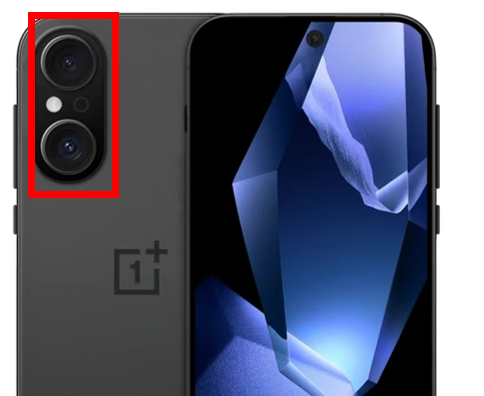
\includegraphics[width=\linewidth]{images/phone_stereocamera.png}
    \caption{手机端双目相机}
    \label{fig:stereo_devices_phone}
  \end{subfigure}\hfill
  \begin{subfigure}[t]{0.32\linewidth}
    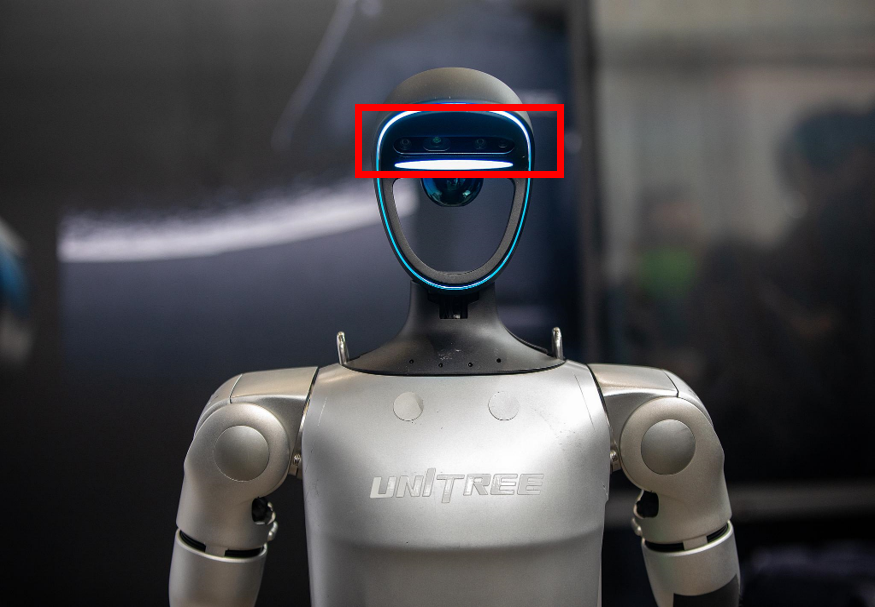
\includegraphics[width=\linewidth]{images/robot_stereocamera.png}
    \caption{机器人双目相机}
    \label{fig:stereo_devices_robot}
  \end{subfigure}\hfill
  \begin{subfigure}[t]{0.32\linewidth}
    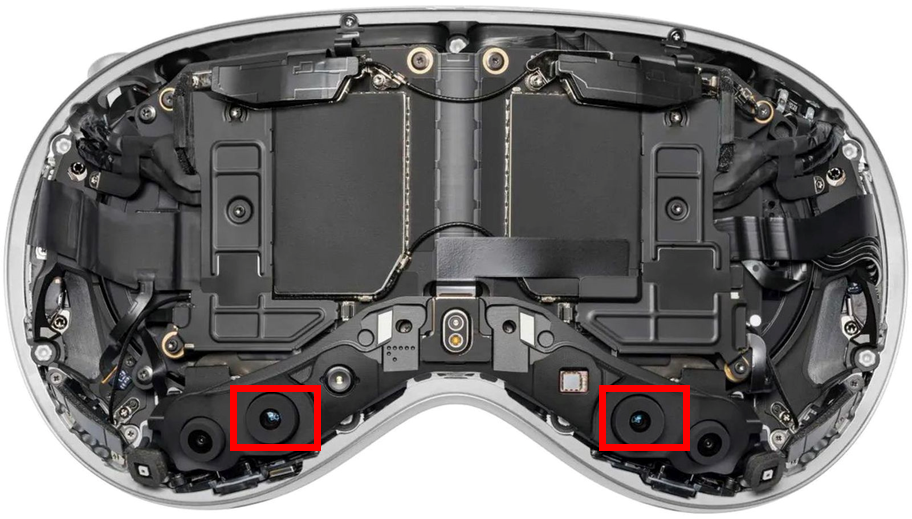
\includegraphics[width=\linewidth]{images/vr_stereocamera.png}
    \caption{VR 头显双目相机}
    \label{fig:stereo_devices_vr}
  \end{subfigure}
  \caption{典型端侧平台中的双目相机应用场景示例（红框标识双目模组）}
  \label{fig:stereo_devices}
\end{figure}

因此，如何在保证双目3D姿态估计精度的前提下，设计轻量化、高效率的网络架构，并结合模型压缩技术实现边缘端的高效部署，是当前学术界与工业界亟待解决的关键问题。一方面，研究者开始探索通过改进网络结构（如引入深度可分离卷积、轻量化注意力机制）来降低计算冗余；另一方面，知识蒸馏和模型量化等技术被广泛证明是在不显著牺牲精度的前提下压缩模型体积、加速推理的有效手段。开展面向资源受限设备的轻量化双目3D人体姿态估计研究，不仅具有重要的学术理论意义，更能推动智能感知技术在移动终端的广泛落地与普惠应用。

\subsection{国内外研究现状}
本节围绕本文研究主线，对 3D 人体姿态估计、双目深度恢复以及端侧轻量化部署三个方面的相关工作进行梳理，并在总结代表性方法的基础上归纳现有研究仍然存在的问题。
\subsubsection{单目 3D 人体姿态估计研究现状}
从传感器配置看，3D 人体姿态估计可大致分为单目、双目与多目三类路线。单目方法硬件成本低、部署灵活，因此长期是三维姿态估计研究的主流方向。

\paragraph{直接回归方法}

Kanazawa 等人提出 HMR\citess{kanazawa2018end}，通过对抗学习将图像特征直接映射为 SMPL 参数，奠定了从单张图像恢复人体三维形状与姿态的经典框架。该方法将人体网格恢复与参数回归统一到同一网络中，推动了基于人体模型先验的单目三维姿态估计研究。

Kolotouros 等人提出 SPIN\citess{kolotouros2019learning}，将基于模型的优化过程嵌入网络训练环节，以 2D 重投影误差持续修正 SMPL 参数，从而提高了人体姿态与形状拟合精度。与直接回归方法相比，该方法更强调“预测 + 迭代优化”的结合，在弱监督场景下表现出更强的参数校正能力。

Li 等人提出 CLIFF\citess{li2022cliff}，针对裁剪后透视信息丢失的问题，将人体在原图中的全局位置信息重新注入网络，使模型能够感知相机视锥并缓解尺度偏差。该工作说明，单目三维人体恢复不仅依赖局部人体外观，还高度受相机成像几何和人体在图像中全局位置的影响。

\paragraph{2D--3D 提升方法}

Martinez 等人提出简洁的全连接基线\citess{martinez2017simple}，证明仅基于二维骨架也可恢复较高质量的三维姿态，为后续 2D--3D 提升方法提供了强有力的基线。该工作弱化了对原始图像纹理的依赖，突出了骨架拓扑先验在三维恢复中的作用。

Pavllo 等人提出 VideoPose3D\citess{pavllo2019videopose3d}，利用时序卷积聚合前后帧信息，有效缓解了单帧估计中的深度歧义与抖动。该方法表明时序上下文对于稳定三维关节轨迹非常关键，尤其适合视频场景下的连续姿态恢复。

Zheng 等人提出 PoseFormer\citess{zheng2021poseformer}，将 Transformer 引入三维姿态提升任务，增强了模型对长时序依赖的建模能力。相比时序卷积结构，该方法更擅长建模远距离帧间关系，但也伴随着更高的计算和存储开销。

在多人场景下，Sun 等人提出 ROMP\citess{sun2021monocular}，利用中心热力图和整图回归策略实现了人数无关的多人三维人体重建，代表了自底向上多人三维姿态估计的一类典型思路。该方法避免了逐人裁剪带来的推理开销增长，但在拥挤场景中的实例分离和遮挡鲁棒性仍是后续工作持续改进的重点。

Zhu 等人提出 MotionBERT\citess{zhu2023motionbert}，以双流并行 Transformer（DSTformer）为骨干构建统一预训练框架，以二维姿态序列为输入进行大规模掩码重建预训练，单一模型可同时迁移至三维姿态估计、动作识别与网格恢复等下游任务，是 ICCV 2023 基于骨架表征预训练的代表性成果。

Gong 等人提出 DiffPose\citess{gong2023diffpose}（CVPR 2023），将三维姿态估计建模为条件扩散生成过程，以 2D 热力图特征为条件通过反向扩散链逐步去噪三维关节坐标，以概率分布自然捕捉深度方向的多义性，是扩散模型在单目三维姿态估计中的开创性工作。

Shin 等人提出 WHAM\citess{shin2024wham}（CVPR 2024），以视频为输入联合恢复人体局部三维姿态与全局世界坐标系轨迹，通过整合脚步接触约束与运动先验实现相机运动与人体运动的解耦，在无需真实相机参数的条件下达到了单目视频全局轨迹重建的前沿性能，代表了单目三维人体运动恢复从相对姿态向绝对轨迹演进的主要趋势。

总体来看，单目方法虽然进展迅速，但其根本困难仍在于深度歧义。仅凭单幅图像，人体尺度变化、自遮挡、视角变化以及复杂背景都可能导致不同三维姿态投影到相近的二维观测，因此在需要绝对空间定位的任务中往往依赖较强的数据先验或额外约束。

\subsubsection{多目 3D 人体姿态估计研究现状}
与单目方法相比，多目系统能够利用跨视图几何一致性显式提供深度线索，因此通常在三维定位精度和遮挡鲁棒性方面更具优势。在多人交互、严重遮挡和大范围动作场景中，不同视角之间的互补观测能够显著降低关键点缺失和深度歧义带来的影响，因此多目方案长期是高精度三维人体姿态估计的重要路线。

Tu 等人提出 VoxelPose\citess{tu2020voxelpose}，将多相机二维热力图提升到统一三维体素空间中联合推理，证明了多视角几何约束对复杂场景三维姿态恢复的有效性。该方法通过把各视角二维观测统一映射到三维空间进行融合，显著提升了多人场景下的三维重建稳定性，体现了多目方法”先在三维空间对齐，再做关节推理”的代表性设计思路。然而体素空间的分辨率与视角数量之积直接决定计算代价，使该类方法在大场景或高帧率场景中面临较大的算力挑战。

针对多目方法在效率与时序一致性上的不足，Choudhury 等人提出 TEMPO\citess{choudhury2023tempo}，采用循环时空架构在单次前向中同时完成多视角姿态估计、人员跟踪与未来姿态预测，通过复用跨帧时序特征避免逐帧重建完整三维体积，在显著降低计算量的同时提升了跨帧的一致性，是多目方法走向实时化的代表性工作。

Srivastav 等人提出 SelfPose3d\citess{srivastav2024selfpose3d}，在完全无三维标注的条件下实现多人多视角三维姿态估计：利用现成的二维检测结果作为伪标签，通过自监督三维人员定位与自监督三维姿态估计双目标协同训练，在 CMU Panoptic、Shelf 及 Campus 等基准上达到与有监督方法相当的精度。该工作显示了多目三维姿态估计在标注成本受限场景中的潜力。

Liao 等人提出 MVGFormer\citess{liao2024multiple}，在 Transformer 框架内引入显式多视角几何推理：以三维查询为中心，将其投影至各视角图像平面，在极线约束引导下聚合跨视图特征，并以可微三角化进行迭代细化，实现了几何感知的端到端训练。实验表明，该方法在跨域泛化（不同相机布局）方面明显优于纯学习式方法，但 Transformer 堆叠带来的算力开销限制了其在资源受限平台上的直接部署。

Chharia 等人提出 MV-SSM\citess{chharia2025mvssm}，以 Mamba 状态空间模型（SSM）替代 Transformer 注意力机制进行多视角融合，设计了带有网格令牌引导双向扫描（GTBS）的投影状态空间（PSS）模块，在保持线性时间复杂度的同时有效建模跨视角长程依赖。该方法在 CMU Panoptic（3 相机）和 Campus 跨域评测上均刷新当前最优精度，是多目三维姿态估计领域的最新进展。

总体来看，多目方法在复杂遮挡和大范围动作场景中通常具有更高的三维恢复上限，但其多相机部署、时间同步和联合标定成本较高，系统搭建与维护复杂度也明显高于单目与双目方案。此外，多目方案往往依赖较固定的相机布局和采集空间，更适合演播室、动作捕捉棚或固定监控区域，而不适合硬件资源和安装条件都更受限制的移动端部署场景。
\subsubsection{双目深度估计与双目三维恢复研究现状}
双目方法的核心在于跨视图对应关系建立与深度恢复。传统立体匹配方法主要依赖手工代价设计与多路径聚合。

Hirschmüller 提出 SGM\citess{hirschmuller2005accurate}，通过沿多方向聚合匹配代价，在精度和效率之间取得较好平衡，成为工业界和工程系统中最常用的经典方案之一。该方法不依赖大规模学习参数，具有较强的工程可实现性，但在弱纹理和遮挡区域仍易出现匹配不稳定。

随着卷积神经网络的发展，双目深度估计逐步从”手工特征 + 后处理”转向”特征提取 + 代价体构建 + 端到端回归”的学习式范式。Kendall 等人提出的 GC-Net\citess{kendall2017end} 率先引入 3D 卷积对代价体进行正则化，Chang 等人的 PSMNet\citess{chang2018psmnet} 进一步以空间金字塔池化和堆叠沙漏结构增强全局上下文建模，Guo 等人的 GwcNet\citess{guo2019gwcnet} 则以分组相关替代拼接以降低代价体构建开销——三者共同奠定了基于代价体学习的立体匹配主流范式，但 3D 卷积带来的计算与显存消耗也成为制约实时化部署的主要瓶颈。

Lipson 等人提出 RAFT-Stereo\citess{lipson2021raft}，以 GRU 迭代更新方式逐步细化视差场，代替了计算代价更高的三维卷积，在跨域泛化能力上明显优于代价体正则化方法。在此基础上，Xu 等人提出 IGEV-Stereo\citess{xu2023igev}（CVPR 2023），构建了融合局部与全局几何信息的联合几何编码体（IGEV），以更紧凑的特征表达支撑 GRU 迭代细化，在 SceneFlow 和 KITTI 基准上以更低计算量超越了 RAFT-Stereo。Wang 等人进一步提出 Selective-IGEV\citess{wang2024selectiveigev}（CVPR 2024），在 IGEV 基础上引入自适应选择机制，对内部几何体与外部上下文特征进行动态融合，取得了 KITTI 2015 排行榜当时最优精度，代表了基于迭代精化的立体匹配的最新进展。

Li 等人提出 STTR\citess{li2021sttr}，将立体匹配建模为序列到序列对应问题，体现了 Transformer 在双目匹配中的应用趋势。该方法强化了对长距离依赖和遮挡区域的建模能力，但自注意力结构对算力和显存的要求较高。

Shamsafar 等人提出 MobileStereoNet\citess{shamsafar2022mobilestereonet}，面向移动端设计轻量化匹配网络，通过削减代价聚合复杂度和优化网络结构，使学习式双目匹配更接近移动端部署需求，在实时性方面取得了更好的工程平衡。

对于本文任务而言，上述立体匹配研究的重要启发在于：双目深度恢复的主流高精度方案大多依赖代价体、全视差搜索和多轮特征聚合，而这些模块恰恰也是端侧部署中最主要的算力与访存开销来源。因此，当双目视觉被用于人体三维姿态恢复时，若仍直接沿用稠密视差估计范式，往往会带来较重的系统负担。这也说明，双目 3D 姿态估计不能简单等同于“人体关键点检测 + 立体匹配”的串联，而需要围绕关节任务重新审视双目交互方式和几何恢复路径。
\subsubsection{双目 3D 人体姿态估计研究现状}
双目 3D 人体姿态估计通常沿“二维关键点检测 + 深度/视差先验 + 三维回代”的路线展开，即先通过双目匹配恢复深度信息，再结合人体关键点位置完成三维关节求解。

Zhang 等人提出 MobiDepthPose\citess{zhang2022mobidepth}，将视频中的人体二维关键点检测与双目深度估计结合，实现了面向移动设备的深度感知三维姿态恢复。该方法体现了”二维姿态 + 深度先验”级联路线在视频场景中的可行性，但其三维精度仍明显受制于前端深度估计质量，且深度与姿态两个模块之间缺乏联合优化。

在工程实践中，另一类常见做法是将 RTMO 等轻量二维姿态检测器与 SGM 或 MobileStereoNet 等双目匹配模块串联，以快速构建可部署的双目三维人体姿态估计系统。该路线模块复用度高、实现直接，但其性能受二维检测误差与深度估计误差的双重影响，且整图密集视差估计的计算成本通常远超关节级三维恢复本身，在端侧场景中效率较低。

值得注意的是，目前专门针对双目相机的端到端三维人体姿态估计研究仍较为匮乏：现有工作或沿用全稠密视差估计的多阶段级联思路，或直接将多视角方法应用于双目设置，鲜有方法从关节任务需求出发重新设计双目特征交互与几何恢复路径。这一研究空白在端侧轻量化部署场景中尤为突出——级联方案的计算冗余与误差传播问题在资源受限设备上被进一步放大，表明设计面向端侧的端到端双目三维姿态估计框架具有重要的实际价值。

总体来看，现有双目 3D 人体姿态估计方法仍以级联方案为主，二维检测误差与深度估计误差容易耦合，整图深度估计开销偏重，这些因素共同限制了其在端侧场景中的进一步优化空间，也正是本文所要重点解决的核心问题。
\subsubsection{常用数据集与评测基准}
三维人体姿态估计的研究进展高度依赖大规模标注数据集的支撑，不同任务场景和研究方向对数据集的规模、视角数量、场景复杂度和标注类型提出了差异化的需求。本节梳理上述研究方向中广泛使用的主要数据集与评测基准。

\textbf{Human3.6M}\citess{ionescu2014human36m} 是三维单人人体姿态估计领域目前最常用的大型室内基准数据集。数据集由 11 名专业演员（6 男 5 女）在受控室内环境下执行讨论、拍照、打电话等 17 种日常活动，通过 4 台同步 RGB 摄像机采集，包含约 360 万帧图像及对应的二维、三维关节标注，同时提供精确的相机内外参数。数据集以 MPJPE（Mean Per Joint Position Error）为主要评价指标，是单目、双目及多视角三维人体姿态估计方法进行横向精度对比的核心标准基准。

\textbf{CMU Panoptic}\citess{joo2015panoptic} 是多视角多人三维人体姿态估计领域最常用的大型基准数据集，由 Joo 等人于 2015 年提出。数据集利用 480 台同步摄像机（包含 RGB 相机和 Kinect 深度相机）在受控穹顶环境中采集了多人社交场景，提供 31 个 RGB 视角的时序数据及三维骨骼标注，覆盖多人互动、交谈等复杂社交行为。该数据集是 VoxelPose、TEMPO、MVGFormer 及 MV-SSM 等多目三维姿态估计方法的主要评测基准。

\textbf{MADS}\citess{zhang2017mads}（Martial Arts, Dancing and Sports Dataset）是专为双目与多视角三维人体姿态估计设计的挑战性数据集，由 Zhang 等人发布。数据集采用一个双目相机及 2 个单目相机（共 4 视角）记录了单人在武术、舞蹈和体育运动场景中的大幅度动作，包含 53\,000 帧 RGB 图像及对应的三维关节真值，提供完整的双目相机内外参数。MADS 是目前少数面向双目相机配置的三维人体姿态估计基准之一，对双目方法的特定评测具有重要参考价值。

\textbf{3DPW}\citess{vonmarcard2018recovering}（3D Poses in the Wild）是首批面向户外复杂场景的三维人体姿态数据集，采用手持单目相机与可穿戴 IMU（惯性测量单元）组合采集，覆盖城市街道、草坪等多种户外环境，包含 5.1 万帧 RGB 图像及对应的 SMPL 三维网格与关节标注。3DPW 主要用于评估模型在自然场景下的跨域泛化能力，常作为单目三维人体恢复方法的域外测试基准。

\textbf{RT-Pose}\citess{ho2024rt} 是 Ho 等人于 2024 年发布的多模态三维人体姿态估计与定位基准数据集（ECCV 2024）。数据集同步采集双路 RGB 相机、非重复水平扫描 LiDAR 及级联成像 4D 雷达三类传感器数据，涵盖 10 名参与者在 40 个场景下（包括室内整洁/杂乱环境以及室外正常天气、雨天和弱光等条件）完成的 6 种不同复杂度动作，共计 7.2 万帧、240 个序列、总时长约 120 分钟，提供与 Human3.6M 兼容的三维骨架标注。三维真值通过将 HRNet 预测的二维关键点输入 ZeDO 优化框架、以 LiDAR 点云辅助根节点深度定位并经人工校验生成，具有较高的标注精度。该数据集的双路 RGB 相机提供了完整的内外参标定信息，支持将其作为双目相机配置用于三维姿态估计，是目前少数同时具备真实室内外场景多样性与精确双目标定的三维人体姿态基准之一。本文在实验中仅使用其双目 RGB 视频流（不使用雷达与 LiDAR 模态），将其作为轻量化双目三维人体姿态估计方法的核心评测基准。

总体来看，各类三维人体姿态估计数据集在场景多样性、视角配置、标注粒度和采集难度上各有侧重：单目方法依赖 Human3.6M 和 3DPW 评测绝对精度与泛化能力，多目方法以 CMU Panoptic 等多相机大型数据集为核心基准，双目方法则因专属基准较少而多借助 MADS 或 Human3.6M 双目配置进行评测。本文主要以 RT-Pose 作为核心训练与评测基准，并以 MADS 作为零样本跨数据集泛化测试集，全面验证所提方法在真实双目场景下的精度与效率。
\subsection{研究内容}
\label{subsec:intro_contribution}

针对现有双目三维人体姿态估计方法在端侧部署中面临的稠密计算冗余与量化适配困难两大核心问题，本文采用软硬件协同设计的研究思路，在网络架构设计阶段即将目标硬件的算子约束、内存访问模式与量化适配性纳入考量，使轻量化算法设计与硬件感知部署形成闭环优化，提出了一套从特征提取、跨视图交互、三维求解到混合精度量化压缩的完整端侧解决方案，具体包含以下两个方面。

\paragraph{轻量化非对称双目三维人体姿态估计网络设计}
鉴于现有双目方案大多沿用"稠密视差估计＋关节回代"的级联思路，存在大量与关节定位无关的像素级计算，且左右对称骨干结构在辅助视角存在明显容量冗余，本文提出了一种轻量化非对称双目学习框架。在骨干设计上，采用"左重右轻"的非对称配置，以大容量主分支负责主视角语义表征，以轻量辅助分支提供稳定的几何观测，并引入跨分支一致性约束保持辅助分支的表征质量。在跨视图交互上，提出极线特征增强模块（EFEM），将跨视图匹配限制在极线约束下的一维视差搜索空间，避免构建全分辨率代价体。在三维恢复上，设计可微加权三角化姿态求解器（DWT），通过 softargmax 提供可微二维观测，并由置信度权重对遮挡或误检视角降权，将热力图分支与几何求解统一到端到端训练链路中。上述架构决策在降低理论计算量的同时，已兼顾目标平台 INT8 量化路径的算子适配性，为后续硬件感知部署提供结构基础。

\paragraph{面向端侧平台的硬件感知量化压缩}
理论参数量与 FLOPs 的降低并不必然转化为真实端侧时延收益，仍需针对目标硬件的算子支持、内存访问模式与数值精度约束进行定向优化。本文面向 Snapdragon~8~Gen3 CPU 平台，首先通过模块级延迟实测与 Roofline 分析定位推理瓶颈（骨干访存受限，EFEM 计算受限），继而通过逐层量化敏感性分析识别精度敏感层（EFEM 注意力激活、热力图头、DWT 求解层），据此制定骨干卷积权重 INT8 量化、敏感层保留 FP32 的分层混合精度方案，并经后训练量化（PTQ）流程输出可在 MNN 框架上运行的部署模型，在真机上验证精度保持与推理加速的有效平衡。
\subsection{论文组织结构}
第一章为绪论。介绍本文的研究背景与现实意义，分析双目3D人体姿态估计在端侧场景中面临的主要挑战，综述国内外相关研究现状，最后阐述本文的研究内容、主要贡献与论文组织结构。

第二章为相关技术与理论介绍。系统梳理本文所依赖的核心理论基础，包括卷积神经网络与Transformer注意力机制等深度学习基础，人体姿态估计的任务范式与评价体系，双目立体视觉的成像模型与极线几何约束，以及面向端侧部署的轻量化结构设计与模型压缩策略。

第三章为基于双目相机的轻量化3D人体姿态检测网络设计。提出一种轻量化非对称双目学习框架：以"左重右轻"的非对称骨干网络消除左右对称冗余，以极线特征增强模块（EFEM）将跨视图匹配限制在一维极线搜索空间，以可微加权三角化求解器（DWT）实现端到端的三维关节坐标恢复，并通过对比实验与消融实验验证各模块的有效性，如图~\ref{fig:system_overview}所示。

第四章为硬件感知部署与量化压缩。面向Snapdragon 8 Gen3端侧平台，通过延迟拆解与Roofline模型定位推理瓶颈，借助量化敏感性分析制定分层混合精度量化方案（骨干INT8、敏感层FP16/FP32），经后训练量化（PTQ）流程输出可部署的MNN模型，在真机上验证精度保持与推理加速效果。

第五章为总结与展望。对全文研究工作进行系统总结，分析现有方法的局限性，并对后续研究方向提出展望。
\begin{figure}[htbp]
  \centering
  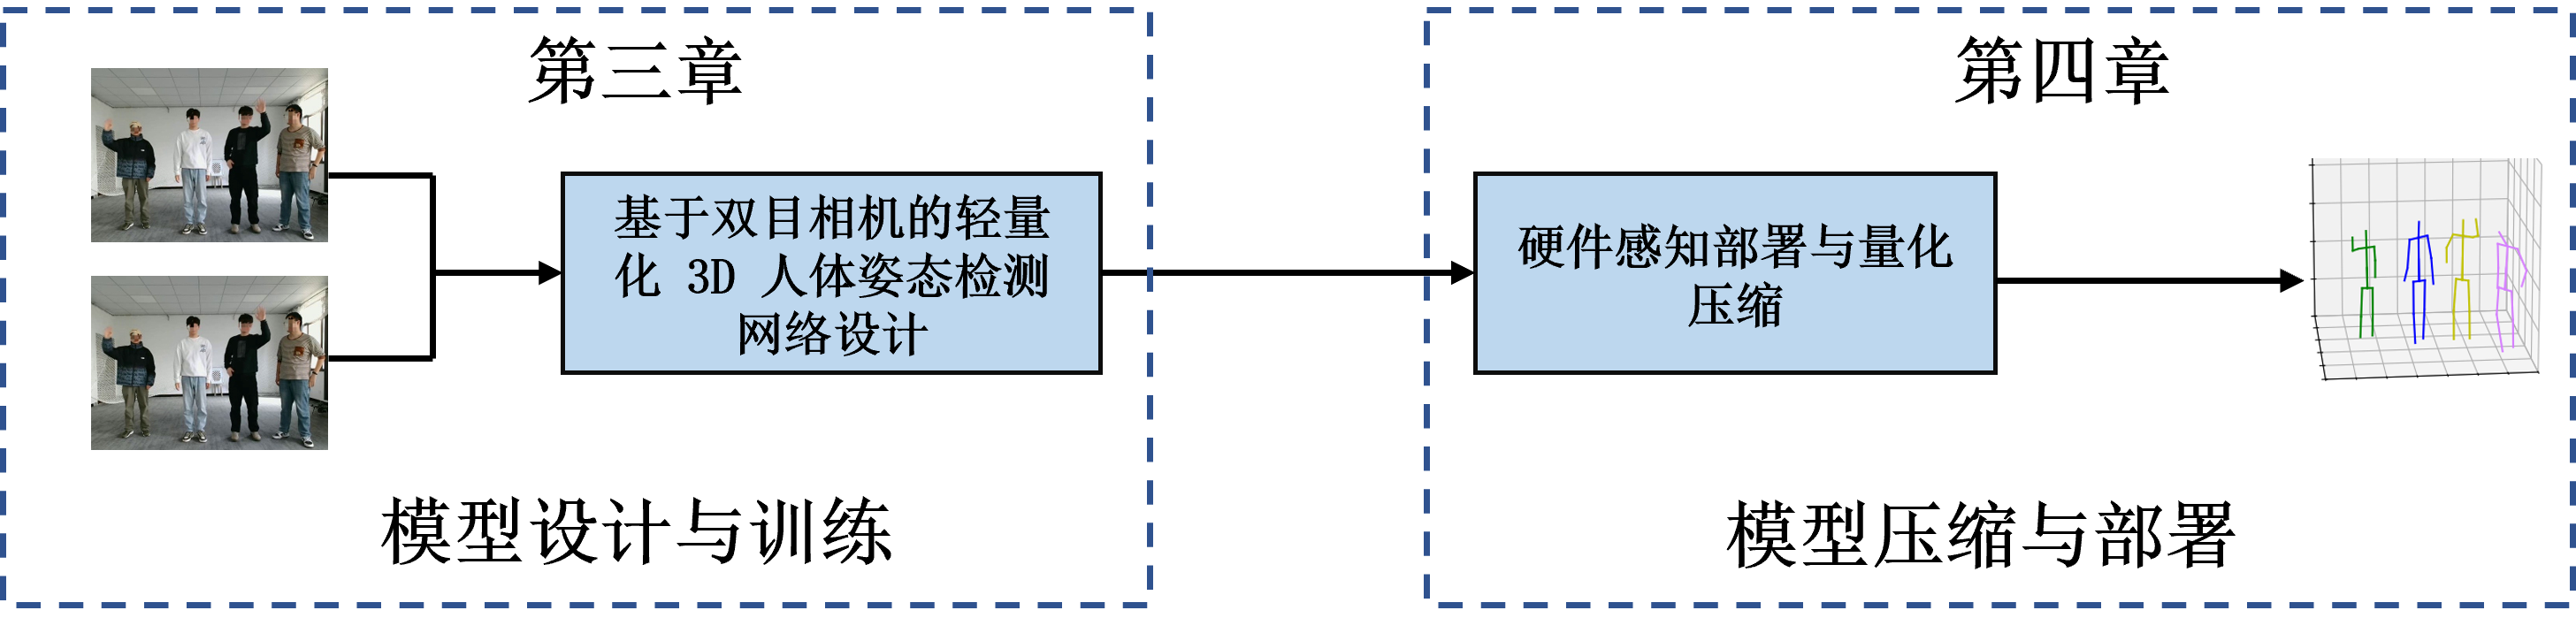
\includegraphics[width=0.85\textwidth]{images/OverallStructureDiagramOfTheSystem.png}
\caption{系统整体结构示意图}
  \label{fig:system_overview}
\end{figure}

\clearpage
\section{相关技术与理论介绍}

本章围绕双目轻量化三维人体姿态估计的研究主线，系统梳理相关核心理论与关键技术，为方法设计与实验分析提供知识铺垫。全章内容分为四个递进部分：第一，介绍卷积神经网络与Transformer注意力机制等深度学习基础，阐述其在视觉特征提取与跨视图信息融合中的作用原理；第二，梳理人体姿态估计的任务范式、关键点表示方法与评价指标体系，明确双目3D姿态估计的输出定义与评测标准；第三，阐述双目立体视觉的成像模型与极线几何约束，介绍三角测量深度恢复的基本原理；第四，总结面向端侧部署的轻量化结构设计原则与模型压缩策略，概述在资源受限设备上实现高效推理的主要技术路径。四部分由浅入深、相互支撑，共同构成本文方法设计与部署优化的知识基础。

\subsection{深度学习基础}\label{subsec:dl_basics}
\subsubsection{卷积神经网络}
卷积神经网络（Convolutional Neural Network, CNN）是一类特殊设计的深度学习模型，它在计算机视觉领域取得了革命性的成功，尤其擅长处理具有网格状拓扑结构的数据，如图像（2D网格）和视频（3D网格）。CNN的核心思想在于通过模仿生物视觉系统的机制，有效利用图像的空间局部相关性，并通过一系列专门的层级结构来学习和提取从低级到高级的层次化特征。
\begin{figure}[htbp]
  \centering
  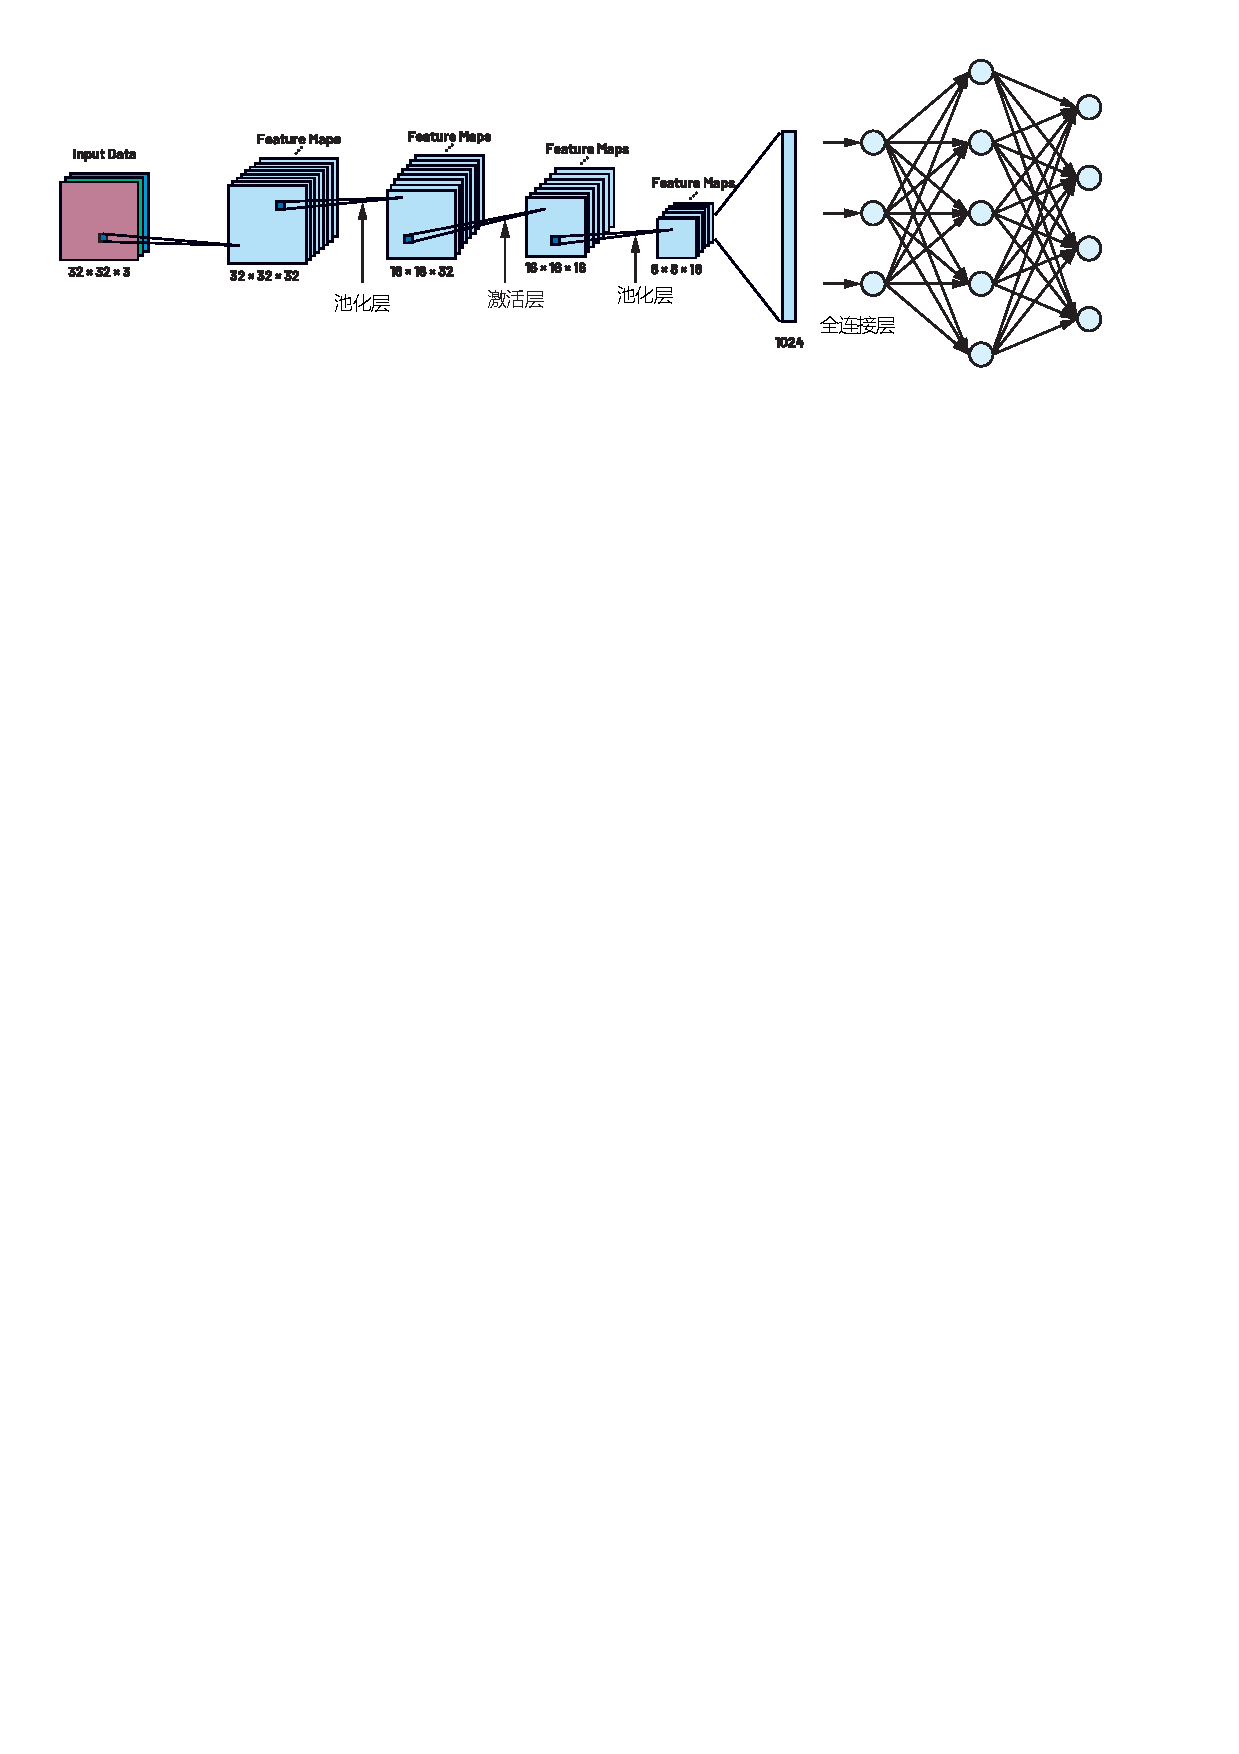
\includegraphics[width=1\textwidth]{images/CNN.pdf}
\caption{典型卷积神经网络架构示意图}
  \label{fig:cnn_architecture}
\end{figure}
典型的CNN架构主要由以下几种关键层堆叠而成：
\paragraph{卷积层 (Convolutional Layer)}
卷积层是CNN的核心。它使用一组可学习的滤波器（或称为卷积核, Kernel）在输入数据（如图像）上进行滑动窗口式的卷积操作。每个卷积核负责检测一种特定的局部特征，例如边缘、角点、纹理或颜色块。通过卷积操作，可以生成一个二维的特征图，图中的每个像素代表了其在原始图像对应感受野（Receptive Field）上对该特定特征的响应强度。卷积层有两个非常重要的特性：

1）局部连接：每个神经元只与输入数据的一个局部区域相连，这大大减少了模型的参数数量，并使网络能专注于学习局部信息。

2）权值共享：单个卷积核（滤波器）在整个输入图像上共享同一组权重参数。这意味着，网络在图像的一个区域学习到的特征（例如，一个垂直边缘），可以同样被用来检测图像其他区域的相同特征。这赋予了模型平移不变性，进一步降低了模型复杂度。

\begin{figure}[h]
  \centering
  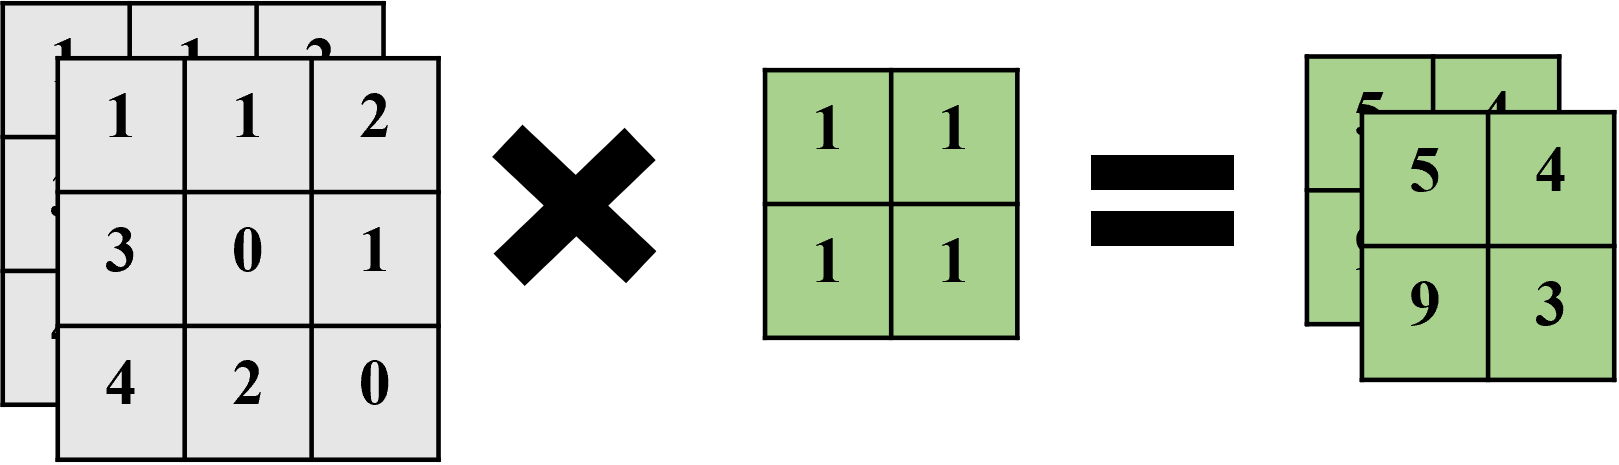
\includegraphics[width=0.5\textwidth]{images/ConvolutionalLayer.png}
\caption{卷积层操作示意图}
  \label{fig:conv_layer}
\end{figure}

\paragraph{激活函数}
在卷积操作之后，通常会应用一个非线性激活函数以引入非线性，从而打破线性模型的表达上限，使网络能够学习更复杂的映射关系。常见激活函数包括 ReLU、Sigmoid 与 Tanh 等。
其中，ReLU (Rectified Linear Unit) 定义为 $f(x)=\max(0,x)$，具有计算开销低、在正半轴梯度不易消失等优点，是卷积网络中最常用的选择之一；Sigmoid 函数定义为
\begin{equation}
\sigma(x)=\frac{1}{1+e^{-x}},
\end{equation}
其输出范围为 $(0,1)$，常用于概率解释或门控结构，但在 $|x|$ 较大时易进入饱和区导致梯度消失；Tanh 函数定义为
\begin{equation}
\tanh(x)=\frac{e^{x}-e^{-x}}{e^{x}+e^{-x}},
\end{equation}
其输出范围为 $(-1,1)$ 且以 0 为中心，相比 Sigmoid 在一定程度上更利于优化，但同样存在饱和导致梯度衰减的问题。

\begin{figure}[h]
  \centering
  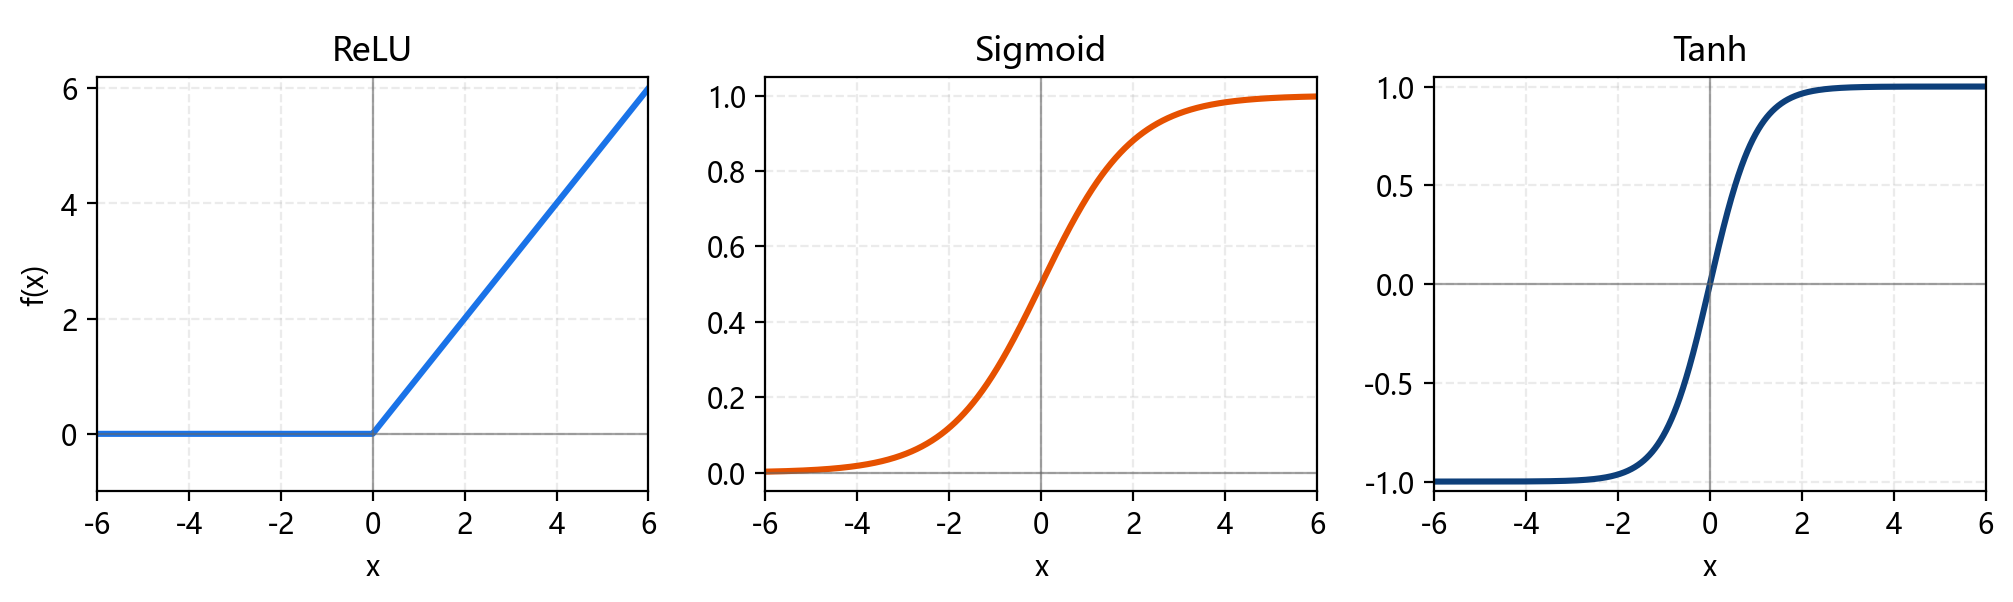
\includegraphics[width=\textwidth]{images/activation_functions.png}
  \caption{三种常见激活函数曲线}
  \label{fig:activation_functions}
\end{figure}

\paragraph{池化层}
池化层（也称下采样层）通常紧跟在卷积层之后，其主要作用是对特征图进行降维，以减少计算量、降低过拟合风险，并增强模型的泛化能力。最常见的池化操作是最大池化（Max Pooling），它将特征图划分为若干个不重叠的矩形区域，并从每个区域中输出最大值。池化操作在保留最显著特征的同时，也为模型带来了一定程度的旋转和尺度不变性。

\begin{figure}[h]
  \centering
  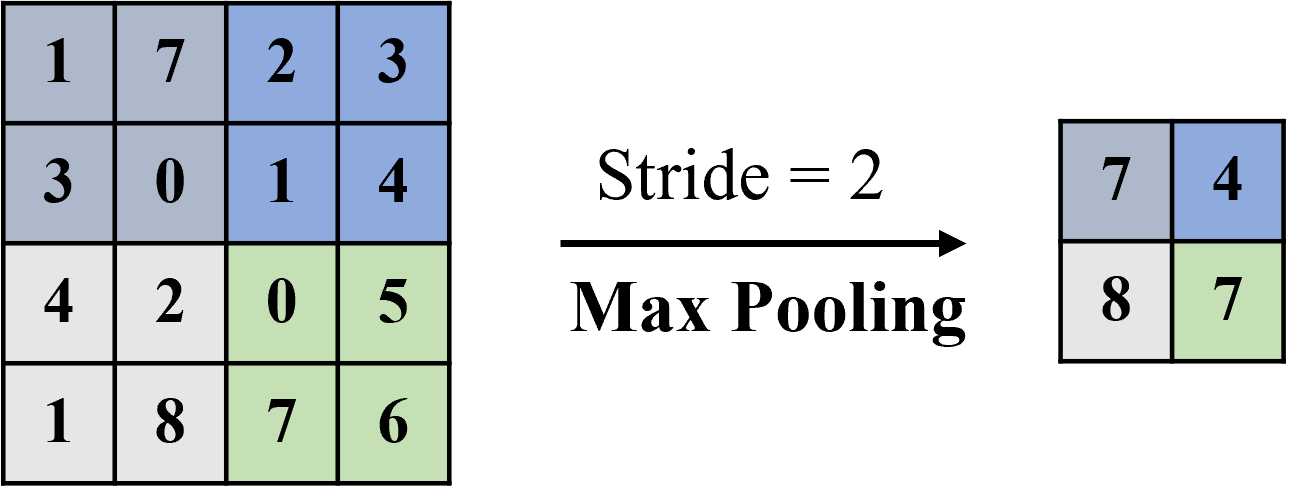
\includegraphics[width=0.5\textwidth]{images/pooling.png}
\caption{池化层操作示意图}
  \label{fig:pooling_layer}
\end{figure}

\paragraph{全连接层}
在经过多层卷积和池化的堆叠，提取出丰富的层次化特征之后，这些特征图通常会被展平（Flatten）成一个一维向量，并输入到一个或多个全连接层中。全连接层的每个神经元都与前一层的所有神经元相连，其作用类似于传统的多层感知机，负责将学习到的分布式特征表示进行整合，并最终映射到任务的输出空间，例如，在分类任务中输出每个类别的概率，或在回归任务（如人体姿态估计）中输出关节点的坐标。

通过这种”卷积-激活-池化”模块的堆叠，CNN能够自动地、层次化地从原始像素中学习到从简单到复杂的视觉模式，使其在图像分类、目标检测、语义分割以及本文所关注的人体姿态估计等任务中表现出色。



\subsubsection{Transformer架构}
Transformer架构最初由Vaswani等人在其著名的论文“Attention Is All You Need”\cite{vaswani2017attention}中提出，旨在解决自然语言处理（NLP）中的序列到序列（Seq2Seq）任务。它摒弃了传统的循环神经网络（RNN）和卷积神经网络（CNN）的序列处理方式，完全依赖于注意力机制来捕捉输入和输出序列之间的全局依赖关系。由于其强大的长距离依赖建模能力和并行计算潜力，Transformer及其变体（如Vision Transformer, ViT\cite{dosovitskiy2020image}）已被成功应用于计算机视觉领域，并在包括人体姿态估计在内的多项任务中取得了SOTA（State-of-the-art）性能。

Transformer的核心是注意力机制，特别是缩放点积注意力（Scaled Dot-Product Attention），其计算可概括为以下公式：
\begin{equation}
\text{Attention}(Q, K, V) = \text{softmax}\left(\frac{QK^\top}{\sqrt{d_k}}\right)V
\end{equation}
其直观计算流程以及多头注意力与 Transformer 整体结构示意如图~\ref{fig:scaled_dot_product_attention} 所示。
\begin{figure}[htbp]
  \centering
  \begin{subfigure}[t]{0.32\linewidth}
    \captionsetup{justification=centering}
    \begin{minipage}[b]{0.7\linewidth}
      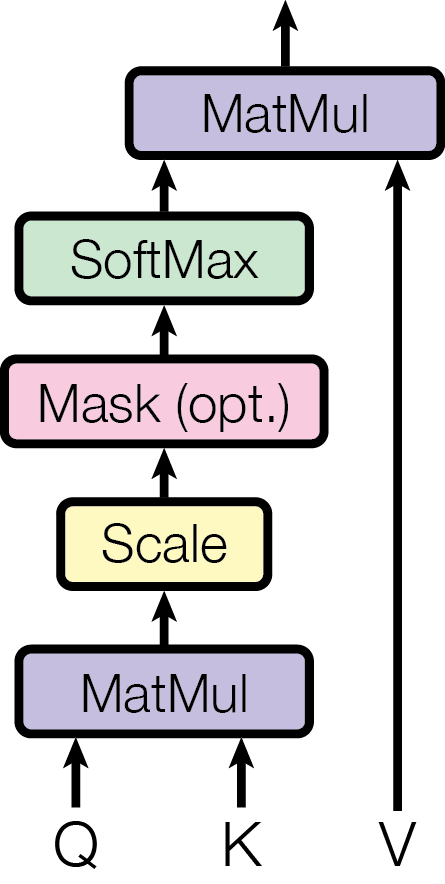
\includegraphics[width=1\linewidth]{images/ScaledDotProductAttention.png}
      \caption{缩放点积注意力}
    \end{minipage}
  \end{subfigure}
  \begin{subfigure}[t]{0.32\linewidth}
    \captionsetup{justification=centering}
    \begin{minipage}[b]{1\linewidth}
      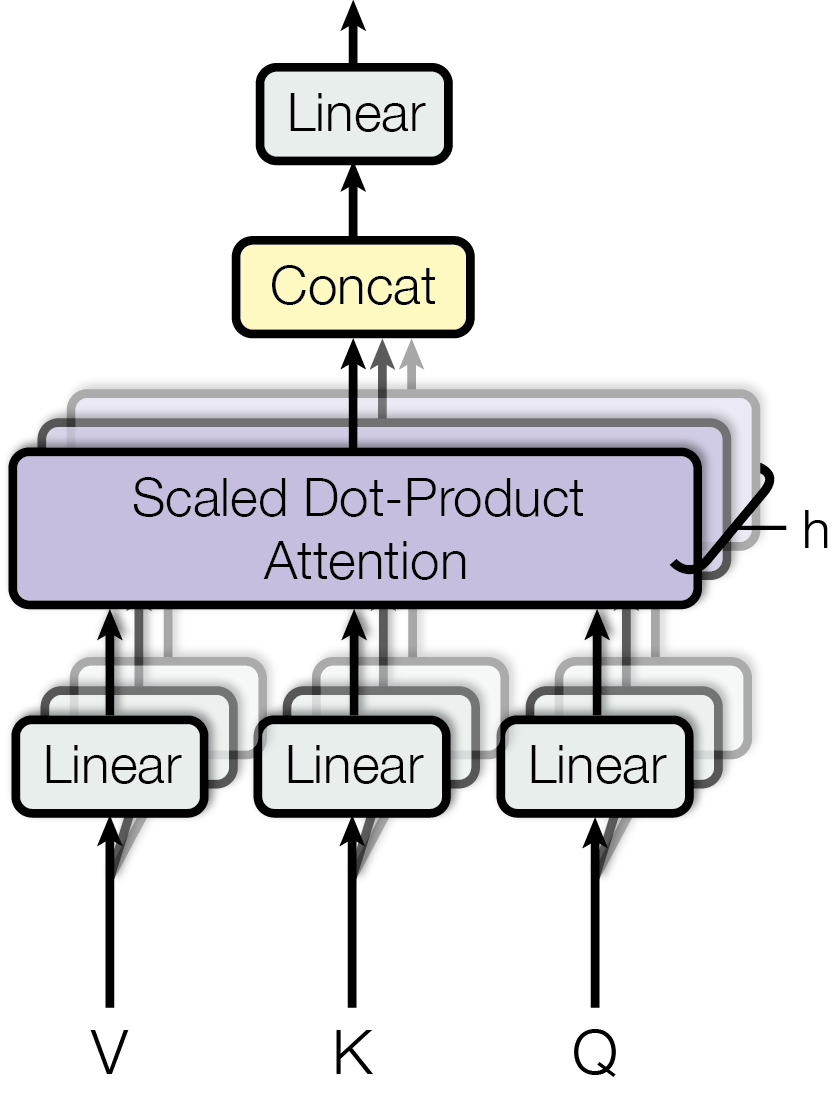
\includegraphics[width=1\linewidth]{images/Mutiheadattention.png}
      \caption{多头注意力}
    \end{minipage}
  \end{subfigure}
  \begin{subfigure}[t]{0.32\linewidth}
    \captionsetup{justification=centering}
    \begin{minipage}[b]{1\linewidth}
      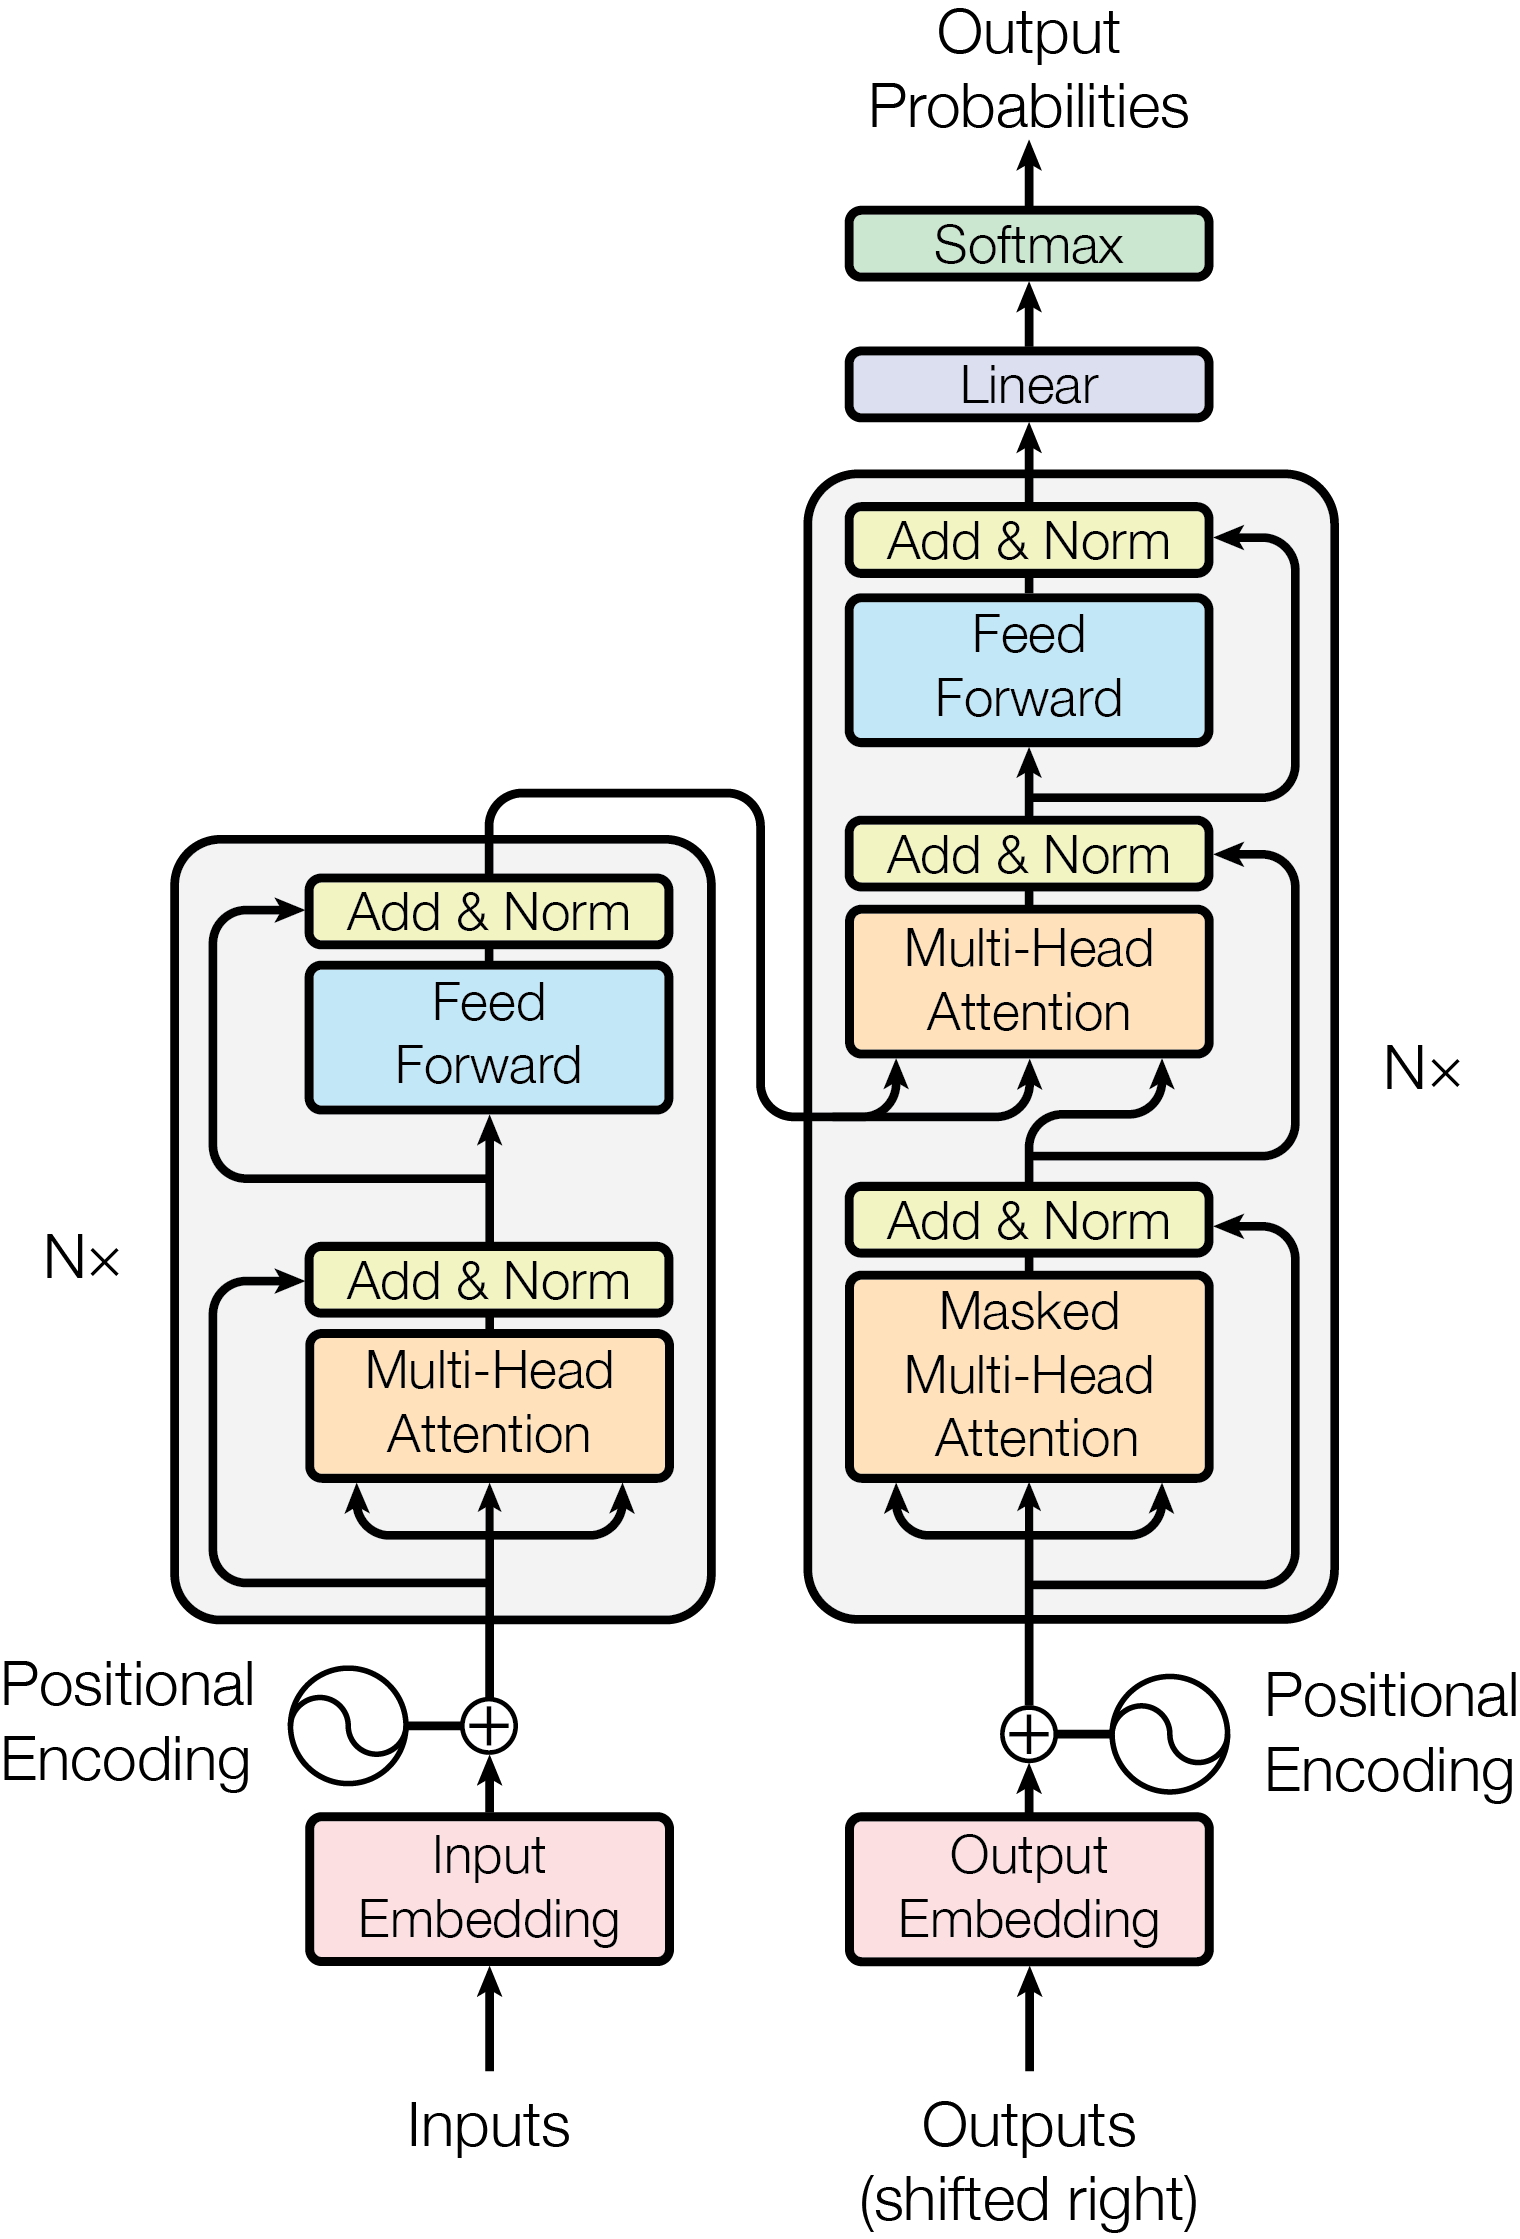
\includegraphics[width=1\linewidth]{images/Transformer.png}
      \caption{Transformer 结构}
    \end{minipage}
  \end{subfigure}
\caption{Transformer 注意力机制与结构示意图}
  \label{fig:scaled_dot_product_attention}
\end{figure}
其中，$Q$（查询）、$K$（键）和$V$（值）是由输入序列经过线性变换得到的三个向量。注意力机制通过计算查询与所有键的相似度（点积），并对结果进行缩放与softmax归一化，得到一组权重系数。这些权重随后被用于对值向量进行加权求和，从而得到最终的输出。这个过程可以直观地理解为：根据“查询”向量$Q$，从一系列“键-值”对（$K\!-\!V$）中检索信息。一个完整的Transformer层通常由一个多头注意力模块和一个前馈神经网络（Feed-Forward Network）组成，每个模块之后都跟随着残差连接（Residual Connection）和层归一化（Layer Normalization）。通过堆叠多个这样的层，Transformer能够构建起强大的深度模型。

\paragraph{自注意力}
自注意力是Transformer中的一个关键特例，其中$Q, K, V$均来自同一个输入序列。这意味着序列中的每个元素都会计算与序列中所有其他元素（包括自身）的注意力权重，从而能够动态地、内容感知地捕捉序列内部的依赖关系，无论它们相隔多远。这与CNN的局部感受野形成了鲜明对比。

\paragraph{多头注意力}
单个注意力头往往只能在一个表示子空间内学习相似性关系，表达能力受限。为同时建模不同尺度、不同语义子空间的依赖，Transformer 引入多头注意力（Multi-Head Attention, MHA）：将输入特征分别线性映射为$h$组不同的$Q,K,V$，并在每个头上独立执行缩放点积注意力，再将各头输出拼接并投影回原维度。其形式化定义为
\begin{equation}
\text{head}_i=\text{Attention}(QW_i^Q,\;KW_i^K,\;VW_i^V),\quad i=1,\dots,h,
\end{equation}
\begin{equation}
\text{MultiHead}(Q,K,V)=\text{Concat}(\text{head}_1,\dots,\text{head}_h)W^O,
\end{equation}
其中$W_i^Q,W_i^K,W_i^V,W^O$为可学习参数矩阵。通常取每个头的维度$d_k=d_{\text{model}}/h$，使总计算量与单头注意力同阶。多头机制的优势在于：不同头可并行关注不同位置与关系模式（例如局部细粒度依赖与全局长程依赖），从而提升模型的表达能力与训练稳定性，并为下游任务提供更丰富的特征融合路径。

\paragraph{交叉注意力}
交叉注意力是连接编码器（Encoder）和解码器（Decoder）的关键桥梁，在标准的Transformer架构中至关重要。与自注意力不同，交叉注意力的$Q$向量来自解码器（Decoder）的输出，而$K$和$V$向量则来自编码器（Encoder）的最终输出。
具体来说，在解码器的每个步骤中，交叉注意力模块允许解码器“关注”输入序列（即编码器的输出）中与当前生成任务最相关的部分。例如，在机器翻译中，当解码器要生成下一个目标词时，交叉注意力会帮助它定位到源句子中最相关的几个词。在多模态任务（如图像描述生成）或本文涉及的双目视觉任务中，交叉注意力机制同样强大。它可以让一个模态的特征（例如，左视图的特征作为查询）去查询和融合另一个模态的特征（例如，右视图的特征作为键和值），从而实现跨模态、跨视图的信息对齐与有效融合。


综合来看，CNN擅长捕捉局部纹理与多尺度空间特征，适合作为高效的视觉骨干网络；Transformer的注意力机制则擅长建立跨位置、跨视图的全局关联。在双目视觉任务中，两类结构相辅相成：CNN负责从左右视图中提取层次化视觉特征，交叉注意力在此基础上实现跨视图特征对齐与极线约束下的信息融合，两者相辅相成，构成双目视觉理解的常见组合框架。

\subsection{人体姿态估计相关理论}\label{subsec:hpe_theory}
\subsubsection{人体姿态估计概述}
人体姿态估计（Human Pose Estimation, HPE）旨在从图像或视频中定位人体关键点（如肩、肘、腕、髋、膝等），并根据预定义的拓扑连接关系构建人体骨架（Pose Skeleton），从而为动作理解、人机交互、康复评估等下游任务提供结构化的运动学表示。

从任务设定上，HPE通常可从以下两个维度进行划分：
（1）按输出维度：分为2D姿态估计（预测关键点平面坐标$ (x,y) $）与3D姿态估计（预测空间坐标$ (x,y,z) $或根相对坐标）。
（2）按目标数量：分为单人姿态估计（Single-person）与多人姿态估计（Multi-person）。

实际应用中，多人拥挤与自/互遮挡会导致关键点可见性显著下降，光照与视角变化及复杂背景会带来跨域分布偏移，从而影响关键点定位的鲁棒性；而在3D姿态估计中，还存在典型的深度歧义性（Depth Ambiguity）问题，即不同的三维姿态可能投影为相似的二维观测，使得仅凭单目图像恢复绝对深度具有不适定性。与此同时，端侧部署还受限于算力、访存与时延预算，要求模型在精度与效率之间取得平衡。基于上述动机，本文聚焦于双目提供绝对尺度线索与轻量化网络端侧部署的统一设计。

\subsubsection{关键点表示方法}
关键点的输出表征直接影响网络结构设计、训练目标与推理开销，常见形式包括：

（1）基于坐标回归（Regression-based）：直接从图像特征回归关键点坐标（或其偏移量）。该方法计算图简单、推理速度快、后处理开销小，适合端侧部署；但由于需要从高维特征到精确坐标的强非线性映射，通常对训练策略与特征表达要求更高，定位精度在复杂场景下可能受限。

（2）基于热图（Heatmap-based）：为每个关键点预测一个二维概率热图，通过峰值位置获得坐标。该方法保留了空间结构信息，定位精度较高，是2D姿态估计的主流范式；但为获得高精度通常需要较高分辨率的特征图与上采样模块，计算与内存开销较大，同时存在由下采样引入的量化误差。

在热图范式中，常用以真值关键点$(u_k,v_k)$为中心生成高斯监督：
\begin{equation}
    H_k(u,v)=\exp\left(-\frac{(u-u_k)^2+(v-v_k)^2}{2\sigma^2}\right)
    \label{eq:gaussian_heatmap}
\end{equation}
其中$\sigma$控制空间扩散范围。当网络输出热图相对输入存在下采样步长$s$时，关键点位置会发生离散化，单轴量化误差上界约为$s/2$，因此端侧系统常需在热图分辨率与计算/内存开销之间进行权衡。

\begin{figure}[h]
  \centering
  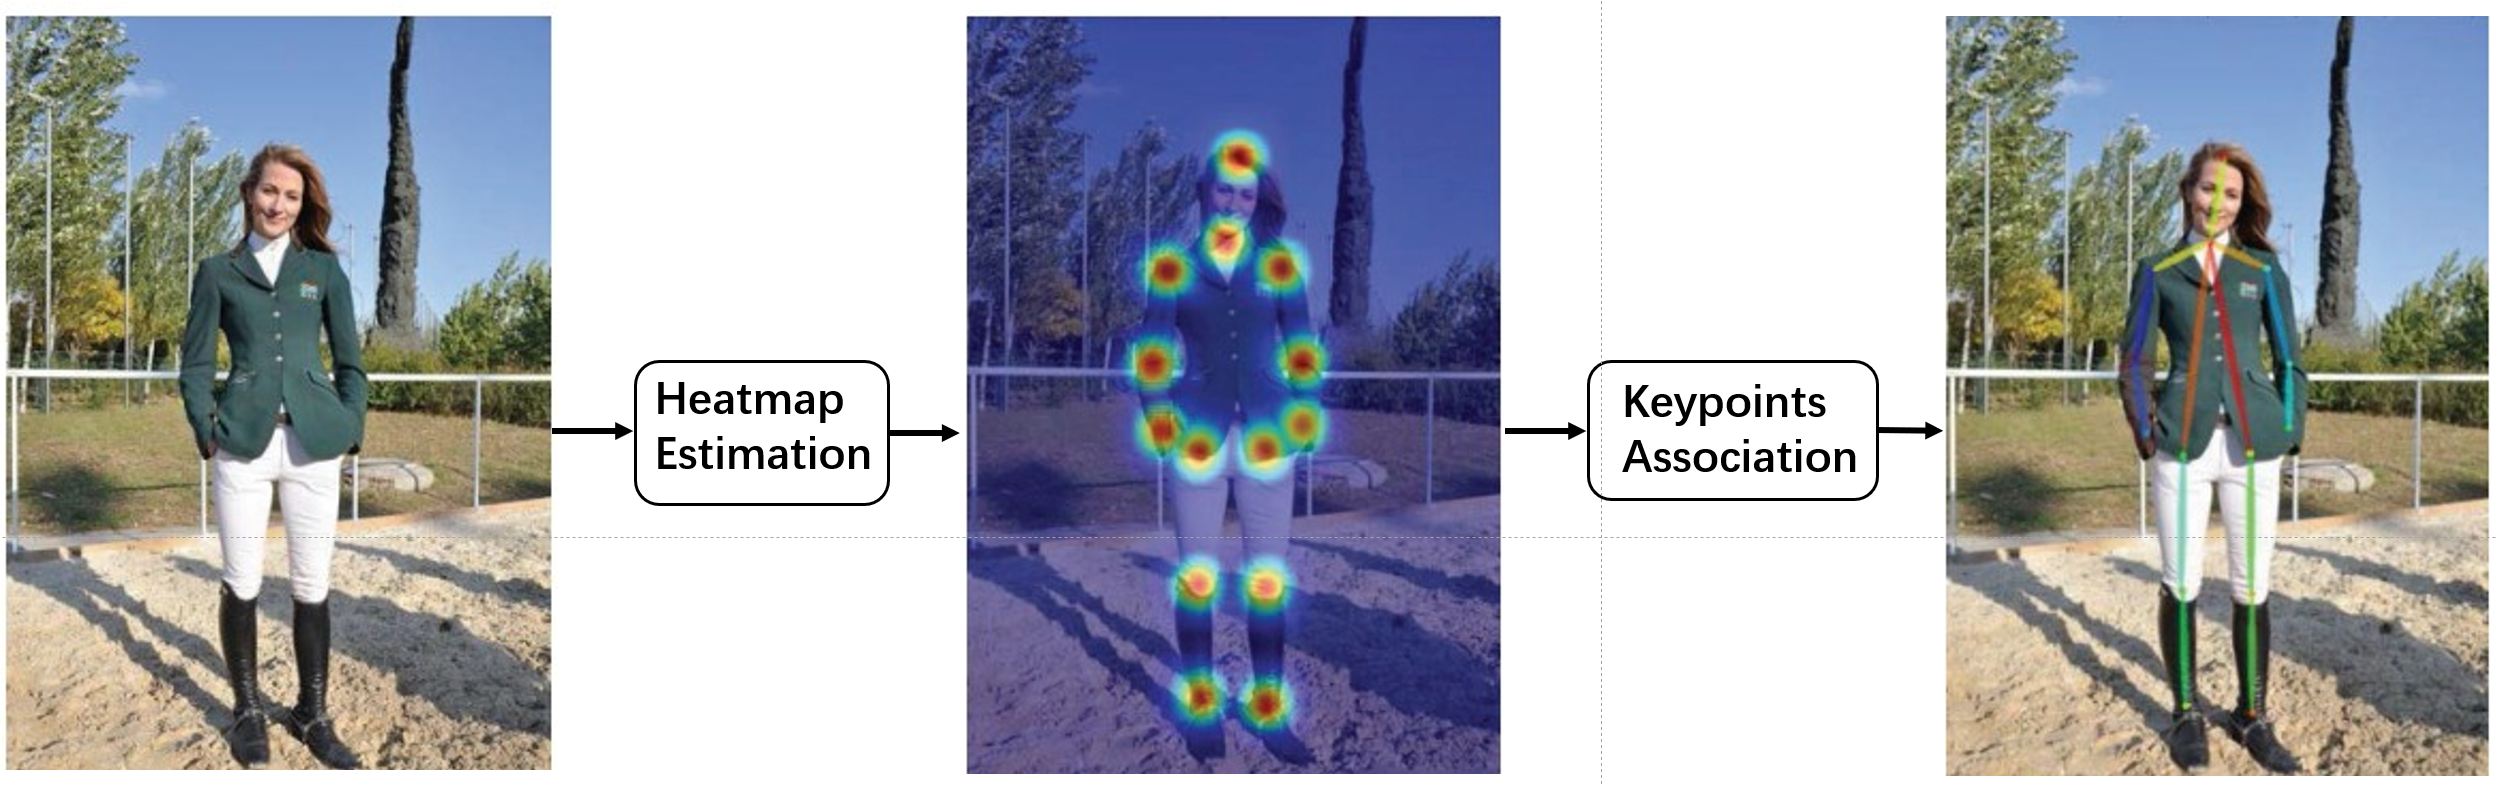
\includegraphics[width=0.85\textwidth]{images/HeatmapBased.png}
\caption{基于热图的人体姿态估计示意图}
  \label{fig:heatmap_based}
\end{figure}

在坐标读出方面，传统$\arg\max$能直接取峰值坐标，但不可导；可导替代方案是soft-argmax（期望读出），例如：
\begin{equation}
    \hat{u}_k=\sum_{u,v} u\cdot \text{softmax}\big(\beta H_k(u,v)\big),\quad
    \hat{v}_k=\sum_{u,v} v\cdot \text{softmax}\big(\beta H_k(u,v)\big)
    \label{eq:softargmax}
\end{equation}
其中$\beta$为温度系数。该读出便于端到端训练，但对热图峰形质量更敏感。综合来看，端侧系统常采用坐标回归或中低分辨率热图+轻量上采样/引导的折中方案，以在时延与精度之间取得更优平衡。

\subsubsection{二维人体姿态估计范式}
二维多人姿态估计主要分为自顶向下与自底向上两类路线：

（1）自顶向下：先使用通用检测器得到人体边界框，再对每个框内执行单人关键点检测。该范式通常精度较高、对尺度变化更鲁棒，例如高分辨率表征学习（HRNet）在关键点定位上表现突出\cite{sun2019deep}；但整体计算量随图像中人数近似线性增长，且性能受检测器误差传递影响。

（2）自底向上：先在整幅图像上检测所有关键点，再通过关联与分组策略将关键点组装成不同的人体实例。OpenPose提出的Part Affinity Fields（PAF）为关键点关联提供了有效表征\cite{cao2017realtime}；该范式推理开销相对稳定，不随人数显著增长，但在严重遮挡、多人拥挤及尺度差异较大时，关键点分组更容易出现歧义。

\begin{figure}[h]
  \centering
  \begin{subfigure}[b]{\textwidth}
    \centering
    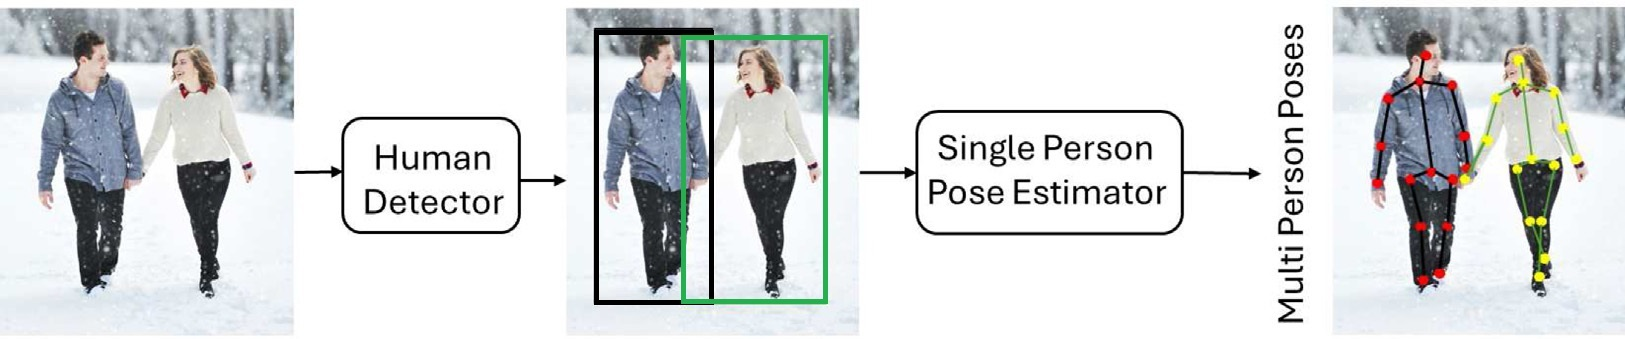
\includegraphics[width=0.9\textwidth]{images/Top-down.jpg}
\caption{自顶向下姿态估计范式}
    \label{fig:topdown}
  \end{subfigure}
  \vspace{0.5em}
  \begin{subfigure}[b]{\textwidth}
    \centering
    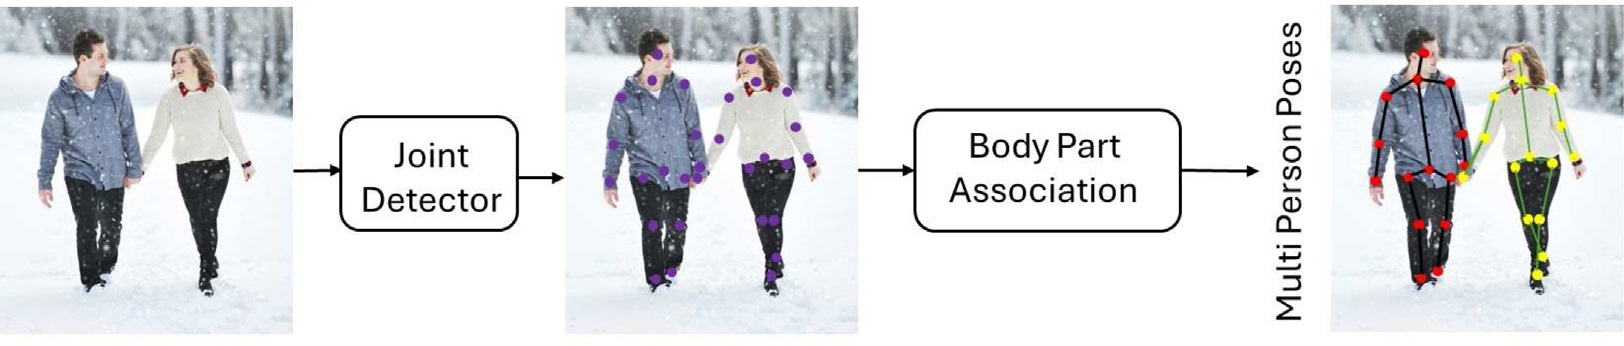
\includegraphics[width=0.9\textwidth]{images/Bottom-up.jpg}
\caption{自底向上姿态估计范式}
    \label{fig:bottomup}
  \end{subfigure}
\caption{二维多人姿态估计主流范式对比}
  \label{fig:pose_paradigms}
\end{figure}

尽管本文的输入为双目图像对，2D关键点检测与热图表征仍可作为中间监督信号或跨视图对齐先验，为后续3D恢复提供更稳定的结构约束。

\subsubsection{三维人体姿态估计方法与坐标口径}
三维人体姿态估计常见方法可归纳为：

（1）端到端直接估计（Direct Estimation）：直接从图像特征回归3D关节点坐标，或进一步回归人体参数化模型（如SMPL）以获得网格与姿态参数\cite{loper2015smpl}。该类方法流程简洁，但往往依赖大量3D标注数据，跨场景泛化能力易受限制。

（2）两阶段法 / 2D到3D提升（2D-to-3D Lifting）：第一阶段获取2D关键点，第二阶段通过提升网络将2D坐标映射到3D空间（可结合时序信息以抑制抖动）。由于第二阶段输入维度低、计算效率高，该路线在轻量化与实时应用中非常常见\cite{martinez2017simple}。

（3）多视图/双目视觉辅助（Stereo/Multi-view）：引入多视角几何约束（如极线约束与三角测量）可显著缓解单目深度歧义，提高3D重建精度与鲁棒性，但对相机标定与同步提出更高要求。本文选择以双目立体几何为基础，在获得绝对尺度线索的同时，将硬件复杂度与跨视图计算控制在更可落地的范围内（详见第\ref{subsec:stereo_principle}节）。

\begin{figure}[h]
  \centering
  \begin{subfigure}[b]{\textwidth}
    \centering
    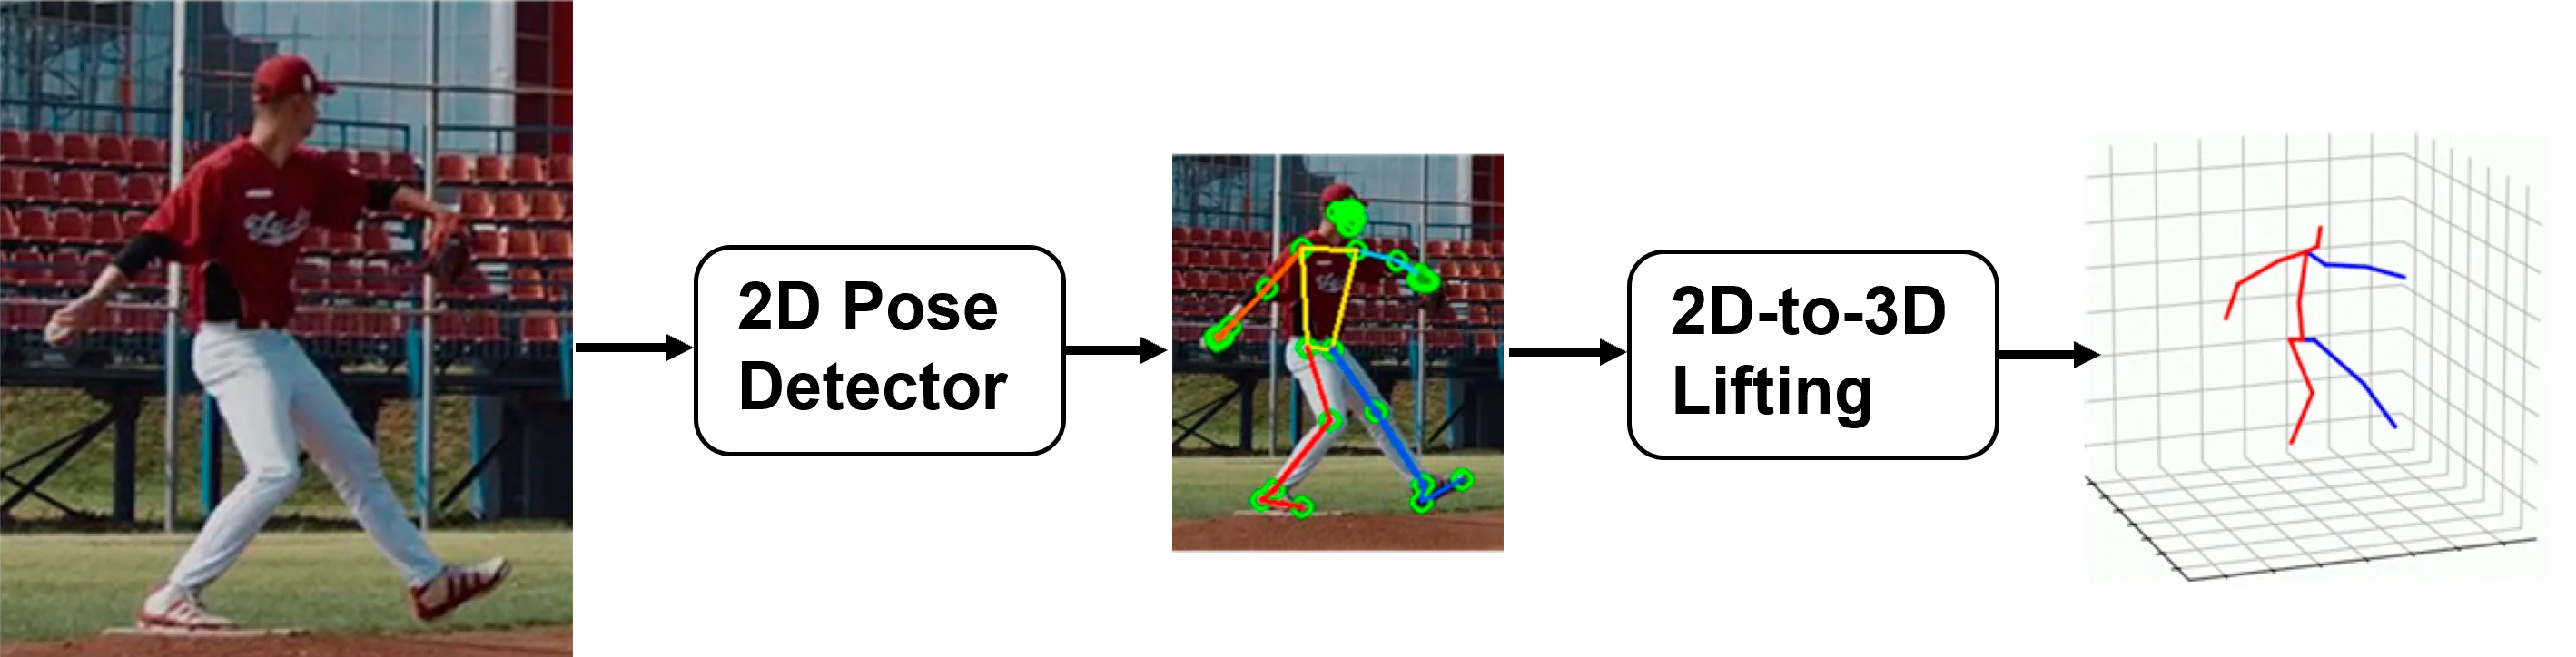
\includegraphics[width=0.85\textwidth]{images/3Dpose_DirectEstimation.png}
\caption{端到端直接估计}
    \label{fig:3d_direct}
  \end{subfigure}
  \vspace{0.5em}
  \begin{subfigure}[b]{\textwidth}
    \centering
    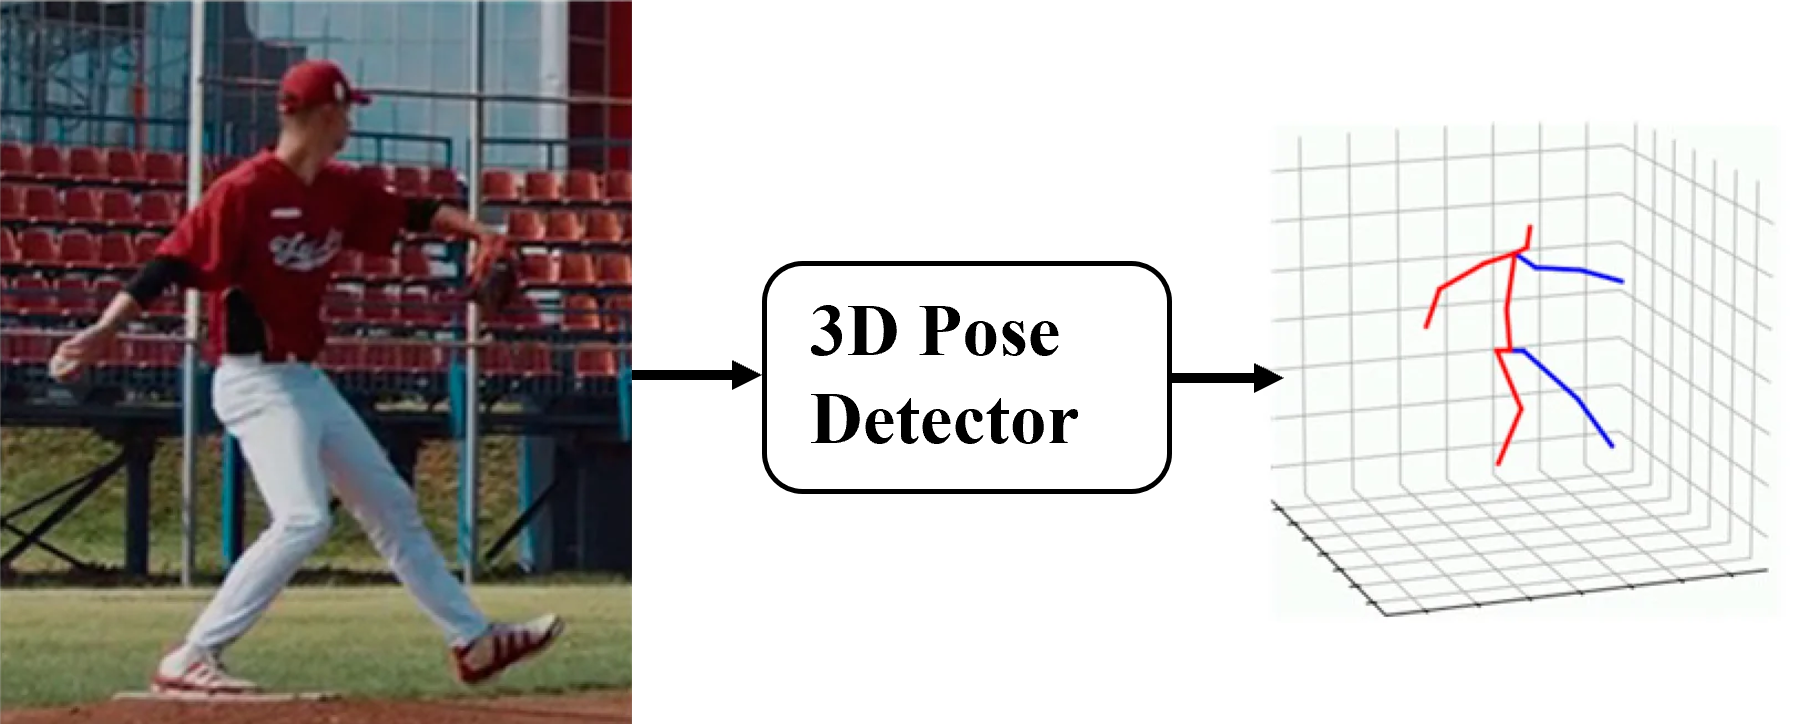
\includegraphics[width=0.5\textwidth]{images/3Dpose_2Dto3D_Lifting.png}
\caption{两阶段 2D 提升法}
    \label{fig:3d_lifting}
  \end{subfigure}
\caption{三维人体姿态估计主流方法示意图}
  \label{fig:3dpose_methods}
\end{figure}

在坐标口径上，3D姿态既可表示为根相对坐标（以骨盆等根节点为原点，消除全局平移影响），也可表示为相机坐标系下的绝对坐标（保留全局位置与尺度）。在双目系统中，标定与三角测量使得绝对尺度可观测，因此本文实验默认在左相机坐标系下报告绝对 MPJPE（mm），而PA-MPJPE等对齐指标更侧重评估姿态形状，可作为补充分析。

此外，注意力机制可显式建模关节间的长距离关系，并在复杂背景中聚焦人体区域；在双目任务中，跨视图注意力（Cross-Attention）可用于左右视图特征对齐与融合，并可与几何先验（如极线约束）结合，将跨视图交互限制在更合理的搜索范围内，从而为后续3D回归提供更一致的表征。

\subsubsection{数据集与评价指标}
\paragraph{常用数据集}
2D姿态估计领域常用公开数据集包括COCO（17个关键点，OKS-mAP评测）\cite{lin2014microsoft}与MPII（16个关键点，PCK评测）\cite{andriluka2014mpii}等；3D姿态估计领域经典数据集包括Human3.6M（室内动作捕捉标注）\cite{ionescu2014human36m}，以及更贴近真实场景的3DPW（in-the-wild）\cite{vonmarcard2018recovering}。在本文实验设置中，RT-Pose数据集用于主要训练与评测\citess{ho2024rt}，MADS数据集用于跨数据集泛化验证\citess{zhang2017mads}。

\paragraph{人体关节点定义与标准}
不同数据集在关节点数量与位置上存在差异：COCO定义17个关节点\cite{lin2014microsoft}，MPII定义16个\cite{andriluka2014mpii}，Human3.6M常用17个核心点\cite{ionescu2014human36m}。在3D姿态表示中，通常以骨盆（Pelvis）为根节点，所有关节点坐标采用根相对（root-relative）方式表示，消除全局位置变化的影响，使模型专注于姿态本身。图~\ref{F.csu_keypoints}展示了典型的人体骨架关节点布局，三套标准的对照关系见表~\ref{tab:pose_comparison}。

\begin{figure}[hbt]
\centering
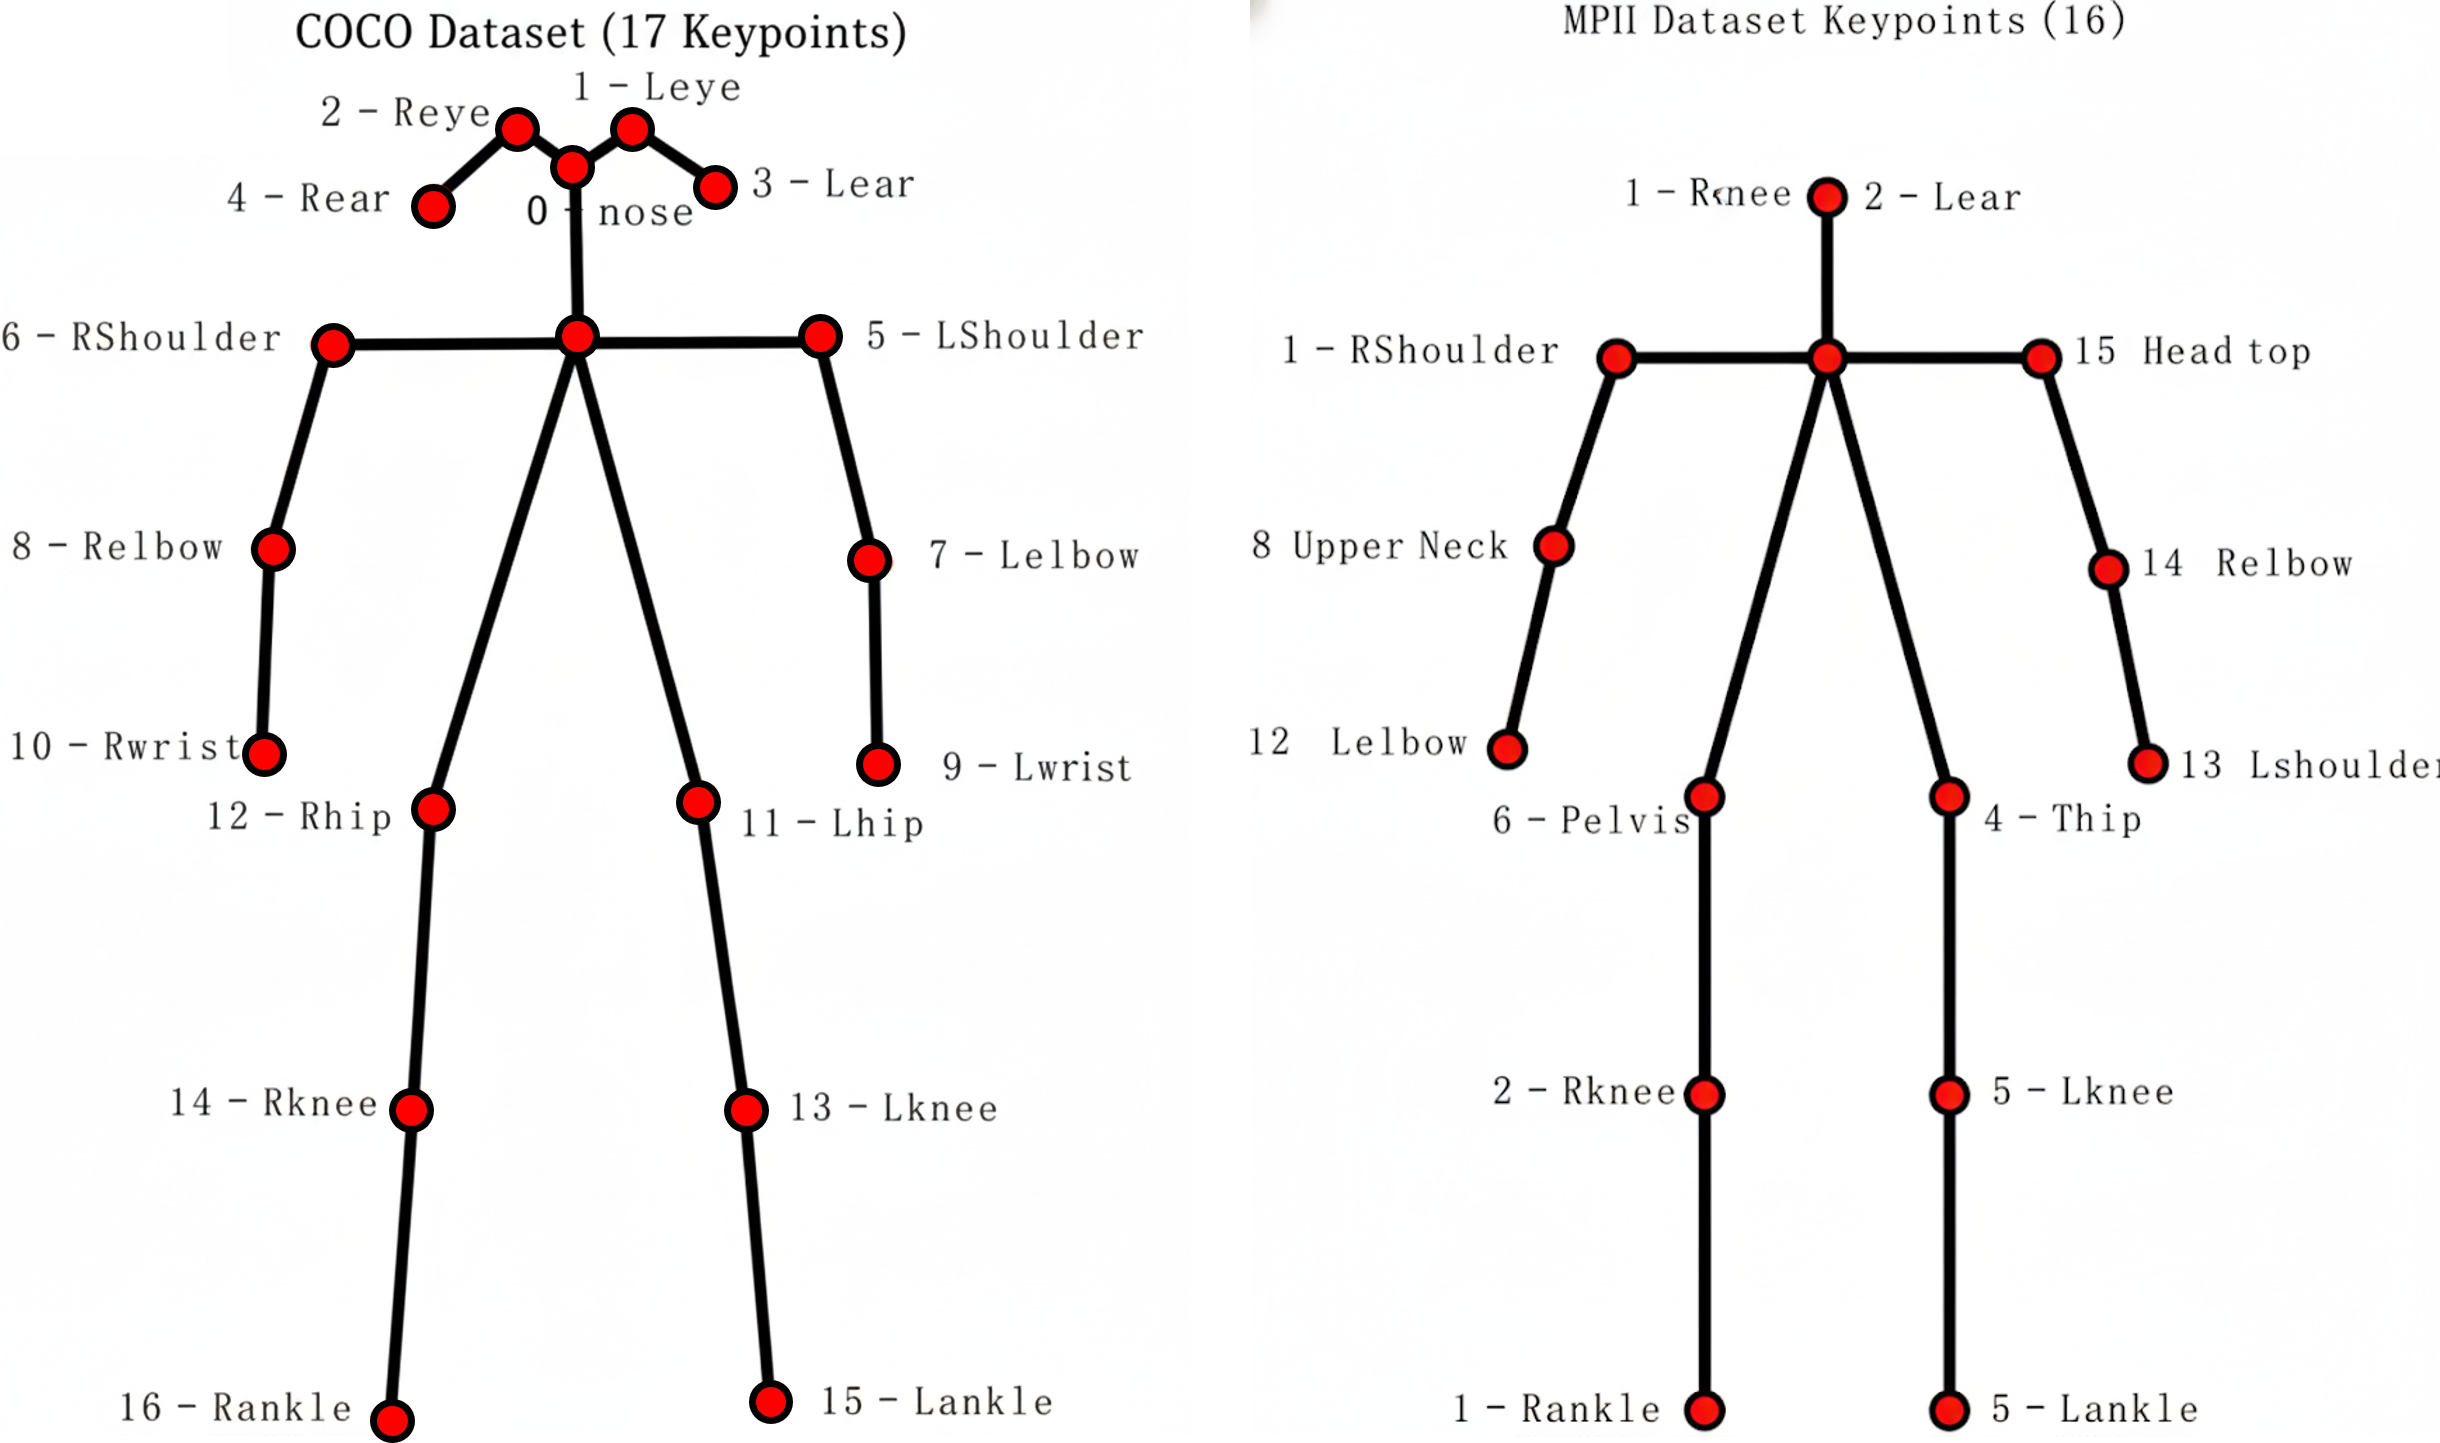
\includegraphics[width=0.8\textwidth]{images/keypoints.png}
\caption{典型的人体关节点骨架示意图}
\label{F.csu_keypoints}
\end{figure}


\begin{table}[ht]
\centering
\caption{COCO\cite{lin2014microsoft}、MPII\cite{andriluka2014mpii}与Human3.6M\cite{ionescu2014human36m}（常用17点）关节点索引对照表}
\label{tab:pose_comparison}
\small
\begin{tabular}{@{}clclcl@{}}
\toprule
Idx & COCO (17) & Idx & MPII (16) & Idx & Human3.6M (17) \\ \midrule
0  & Nose (鼻子)       & 0  & R-Ankle (右踝)   & 0  & Pelvis (骨盆/中心) \\
1  & L-Eye (左眼)      & 1  & R-Knee (右膝)    & 1  & R-Hip (右臀)      \\
2  & R-Eye (右眼)      & 2  & R-Hip (右臀)     & 2  & R-Knee (右膝)     \\
3  & L-Ear (左耳)      & 3  & L-Hip (左臀)     & 3  & R-Ankle (右踝)    \\
4  & R-Ear (右耳)      & 4  & L-Knee (左膝)    & 4  & L-Hip (左臀)      \\
5  & L-Shoulder (左肩) & 5  & L-Ankle (左踝)   & 5  & L-Knee (左膝)     \\
6  & R-Shoulder (右肩) & 6  & Pelvis (骨盆)    & 6  & L-Ankle (左踝)    \\
7  & L-Elbow (左肘)    & 7  & Thorax (胸部)    & 7  & Torso (躯干)      \\
8  & R-Elbow (右肘)    & 8  & Upper Neck (颈)  & 8  & Neck (颈部)       \\
9  & L-Wrist (左腕)    & 9  & Head Top (头顶)  & 9  & Nose (鼻子/头)    \\
10 & R-Wrist (右腕)    & 10 & L-Wrist (左腕)   & 10 & Head (头顶)       \\
11 & L-Hip (左臀)      & 11 & L-Elbow (左肘)   & 11 & L-Shoulder (左肩) \\
12 & R-Hip (右臀)      & 12 & L-Shoulder (左肩) & 12 & L-Elbow (左肘)    \\
13 & L-Knee (左膝)     & 13 & R-Shoulder (右肩) & 13 & L-Wrist (左腕)    \\
14 & R-Knee (右膝)     & 14 & R-Elbow (右肘)   & 14 & R-Shoulder (右肩) \\
15 & L-Ankle (左踝)    & 15 & R-Wrist (右腕)   & 15 & R-Elbow (右肘)    \\
16 & R-Ankle (右踝)    & -- & --               & 16 & R-Wrist (右腕)    \\ \bottomrule
\end{tabular}
\end{table}

\paragraph{评价指标}
人体姿态估计任务通常通过一系列量化指标进行评估。对于2D姿态估计，常用指标包括（以MPII\cite{andriluka2014mpii}与COCO\cite{lin2014microsoft}评测口径为例）：
（1）PCK（Percentage of Correct Keypoints）：统计预测关键点落在归一化阈值范围内的比例，阈值通常根据人体尺度（如头部尺寸或躯干长度）进行归一化\cite{andriluka2014mpii}。

（2）OKS（Object Keypoint Similarity）：综合考虑关键点像素误差、可见性以及不同关键点标注不确定性，用于更细致地衡量关键点相似度\cite{lin2014microsoft}。

（3）mAP：基于OKS阈值统计平均精度，是COCO评测中最常用的2D姿态指标\cite{lin2014microsoft}。
对于3D人体姿态估计，最核心和最广泛使用的指标之一是平均每关节位置误差（Mean Per Joint Position Error, MPJPE）。

\subparagraph{MPJPE (Mean Per Joint Position Error)}
MPJPE，有时也称为重构误差（Reconstruction Error），是衡量3D人体姿态估计精度的金标准。它计算的是模型预测的3D关节点坐标与真实3D关节点坐标（Ground Truth）之间的平均欧氏距离（Euclidean Distance）。如公式\ref{eq:mpjpe}所示，对于一个包含$N$个关节点的姿态，其MPJPE的计算方式如下：
\begin{equation}
\text{MPJPE} = \frac{1}{N} \sum_{i=1}^{N} \left\| J_{pred, i} - J_{gt, i} \right\|_2
\label{eq:mpjpe}
\end{equation}
其中，$J_{pred, i}$和$J_{gt, i}$分别代表第$i$个预测关节点和真实关节点的3D坐标。这个值通常以毫米（mm）为单位，其值越低，代表模型的预测精度越高。本文实验默认报告绝对 MPJPE：在左相机坐标系下直接计算预测三维关节与真值三维关节的欧氏距离（mm）；根相对 MPJPE 或仅尺度对齐（scale-aligned）的误差可作为可选补充指标，用于分析全局平移/尺度因素的影响。

\subparagraph{PA-MPJPE (Procrustes Aligned MPJPE)}
然而，在某些场景下，我们更关心模型预测的姿态形状（Shape）的准确性，而非其在空间中的全局位置、旋转和缩放。例如，一个预测的姿态可能在形状上与真实姿态完全一致，但由于整体平移或旋转，其MPJPE值仍然会很高。为了消除这种全局变换带来的影响，研究者们提出了Procrustes对齐后的MPJPE（PA-MPJPE），也称形状误差（Shape Error）。

在计算PA-MPJPE之前，需要通过刚性变换（旋转、平移和缩放），即Procrustes分析，将预测的3D姿态与真实3D姿态进行对齐。PA-MPJPE计算的是在最佳对齐之后，预测关节点与真实关节点之间的平均欧氏距离。其计算公式如下：
\begin{equation}
\text{PA-MPJPE} = \min_{R, t, s} \frac{1}{N} \sum_{i=1}^{N} \left\| (sR \cdot J_{pred, i} + t) - J_{gt, i} \right\|_2
\end{equation}
其中，优化过程寻找一个最佳的旋转矩阵$R$、平移向量$t$和缩放因子$s$，以最小化对齐后的平均误差。PA-MPJPE能够更纯粹地评估模型对人体结构和比例的学习能力，是衡量姿态“形状”准确性的关键指标。




\subsection{双目立体视觉原理}
\subsubsection{双目立体视觉成像模型}
\label{subsec:stereo_principle}
双目立体视觉通过两台相机从不同视角同时观测同一场景，利用左右视图之间的几何约束恢复场景的深度信息。设空间点在世界坐标系中的齐次坐标为$\mathbf{X}=[X,Y,Z,1]^\top$，其在左/右相机成像平面上的齐次像素坐标分别为$\mathbf{x}_l=[u_l,v_l,1]^\top$与$\mathbf{x}_r=[u_r,v_r,1]^\top$，则在针孔相机模型下有：
\begin{equation}
s_l \mathbf{x}_l = \mathbf{K}_l \left[\mathbf{R}_l \ \mathbf{t}_l\right]\mathbf{X}, \quad
s_r \mathbf{x}_r = \mathbf{K}_r \left[\mathbf{R}_r \ \mathbf{t}_r\right]\mathbf{X}
\label{eq:stereo_projection}
\end{equation}
其中，$\mathbf{K}$为相机内参矩阵（包含焦距与主点），$\left[\mathbf{R}\ \mathbf{t}\right]$为外参（描述相机坐标系相对世界坐标系的旋转和平移），$s$为尺度因子。双目系统通常通过标定获得两台相机的内参及它们之间的相对位姿，其中两相机光心之间的距离称为基线（Baseline）$B$。

\subsubsection{极线几何与立体校正}
如图~\ref{fig:epipolar_geometry}所示，在双目系统中，左右相机光心$C_l$与$C_r$以及空间点$\mathbf{X}$共同确定一个对极平面（Epipolar Plane）。对极平面分别与左右成像平面相交得到极线$l_l$与$l_r$；另一相机光心在本相机成像平面上的投影为对极点$e_l$与$e_r$，且任意极线必过对应对极点。由此可知，当左图像点$\mathbf{x}_l$已知时，其在右图像中的对应点$\mathbf{x}_r$不再是二维搜索，而被约束在右图极线$l_r$上（反之亦然），这正是极线约束降低匹配复杂度的几何本质。

\begin{figure}[htbp]
  \centering
  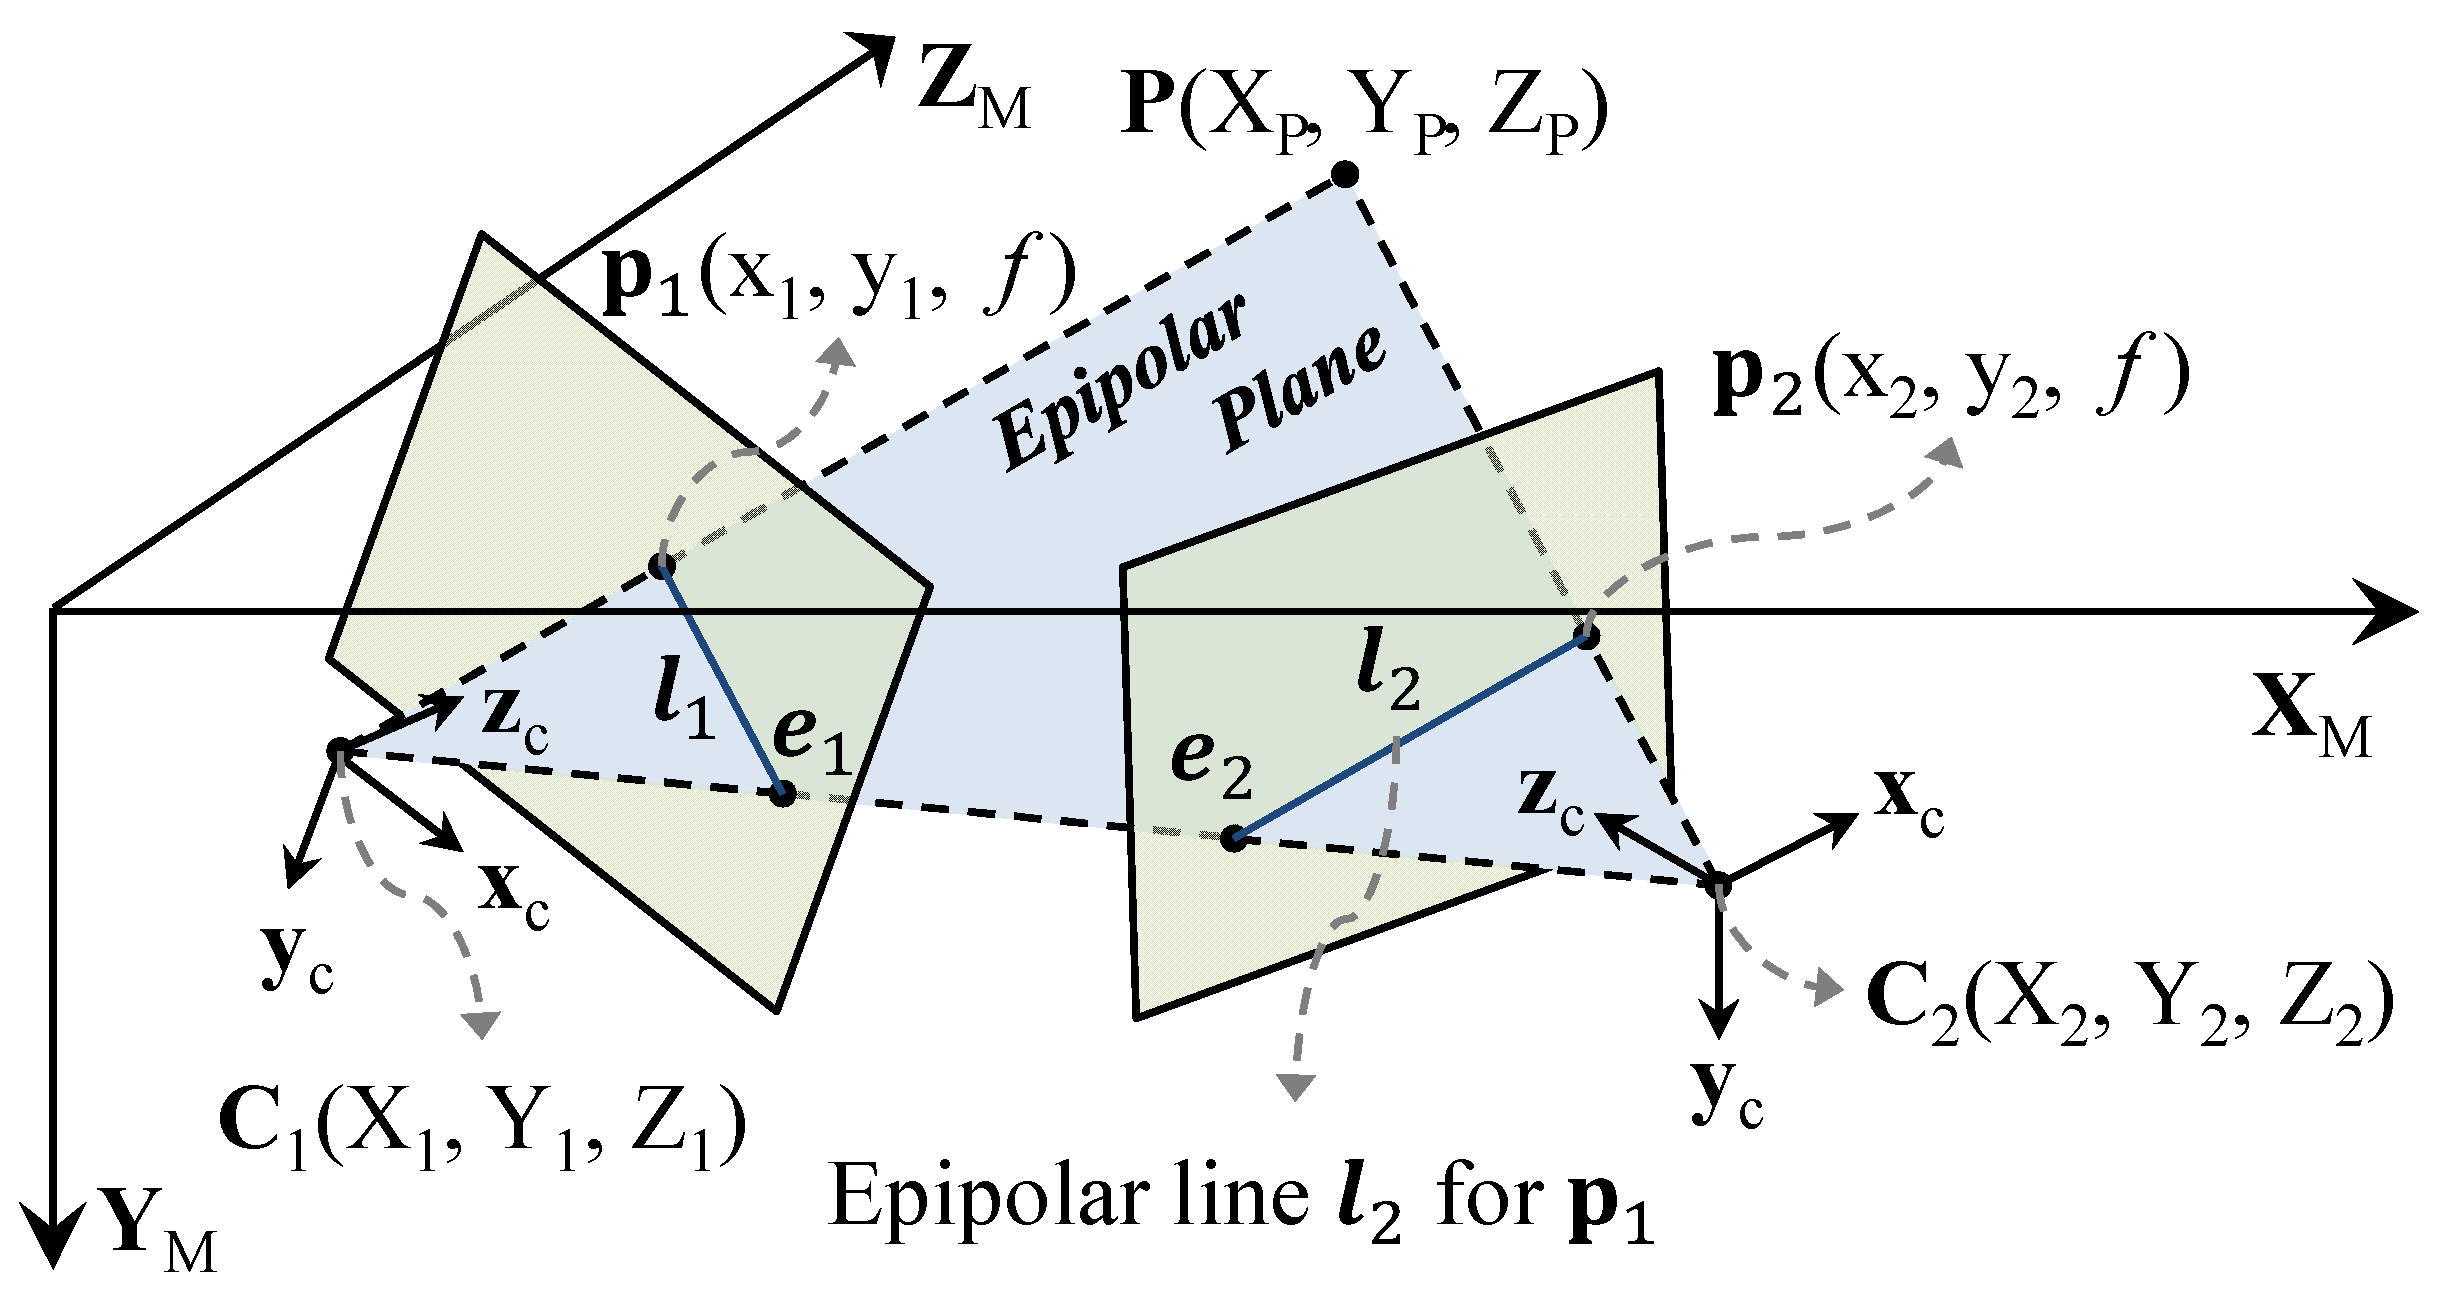
\includegraphics[width=0.8\textwidth]{images/EpipolarGeometry.png}
\caption{双目对极几何示意图}
  \label{fig:epipolar_geometry}
\end{figure}

图中，$\mathbf{x}_l=[u_l,v_l,1]^\top$与$\mathbf{x}_r=[u_r,v_r,1]^\top$分别为$\mathbf{X}$在左右成像平面上的像素齐次坐标，通过各自相机内参矩阵$\mathbf{K}$与归一化相机坐标关联（$\mathbf{x}\sim\mathbf{K}\tilde{\mathbf{x}}$）。

对于同一空间点$\mathbf{X}$在左右视图中的像素对应$\mathbf{x}_l$与$\mathbf{x}_r$，其匹配关系满足极线约束：
\begin{equation}
\mathbf{x}_r^\top \mathbf{F}\mathbf{x}_l = 0
\label{eq:epipolar_constraint}
\end{equation}
其中$\mathbf{F}$为基础矩阵（Fundamental Matrix）。对于已标定的双目系统，两相机间的相对旋转$\mathbf{R}$与平移$\mathbf{t}$已知，可先构造本质矩阵（Essential Matrix）：
\begin{equation}
\mathbf{E} = [\mathbf{t}]_\times \mathbf{R}
\label{eq:essential_matrix}
\end{equation}
其中$[\mathbf{t}]_\times$为$\mathbf{t}$的反对称矩阵。基础矩阵则由本质矩阵与左右相机内参联合给出：
\begin{equation}
\mathbf{F} = \mathbf{K}_r^{-\top}\,\mathbf{E}\,\mathbf{K}_l^{-1}
\label{eq:fundamental_matrix}
\end{equation}
上式表明，$\mathbf{F}$完全由标定参数$\{\mathbf{K}_l,\mathbf{K}_r,\mathbf{R},\mathbf{t}\}$决定。工程实现中通常对左右图像进行立体校正（Stereo Rectification）：将倾斜的极线变换为水平扫描线，使校正后对应点满足$v_l = v_r$，跨视图匹配从二维搜索退化为一维水平扫描，视差$d = u_l - u_r$成为唯一待估量，自然引出下一节的三角测量深度恢复。

\subsubsection{视差与深度恢复（三角测量）}
在完成立体校正且双目相机近似共面、光轴平行的情况下，视差定义为左右像素横坐标之差：
\begin{equation}
d = u_l - u_r
\label{eq:disparity_def}
\end{equation}
由相似三角形关系可得空间点的深度（以左相机坐标系为例）：
\begin{equation}
Z = \frac{f B}{d}
\label{eq:depth_from_disparity}
\end{equation}
其中$f$为等效焦距（通常使用$ f_x $），$B$为基线长度。由式\ref{eq:depth_from_disparity}可知：深度与视差成反比，近处物体具有更大的视差、更易估计；远处物体视差很小，对匹配误差更敏感。图~\ref{fig:triangulation}给出了双目视差与三角测量的几何关系示意。

\begin{figure}[htbp]
\centering
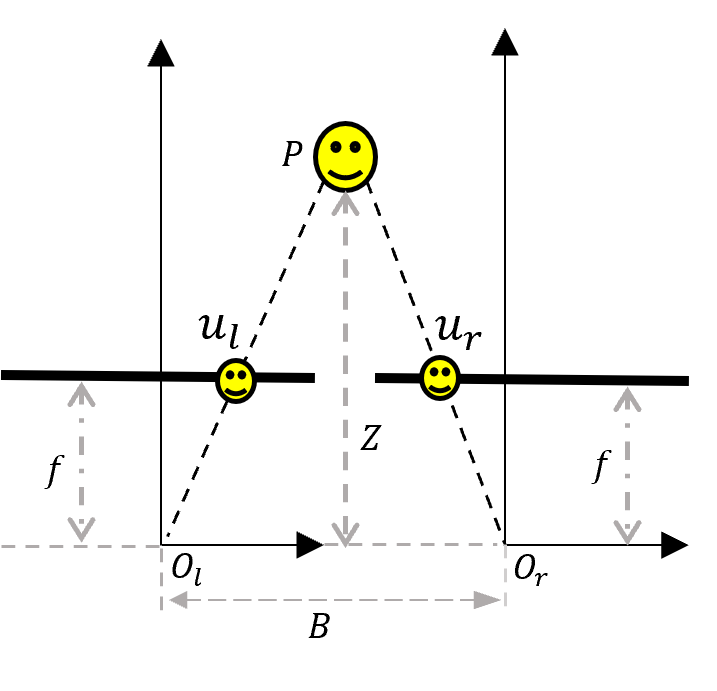
\includegraphics[width=0.5\textwidth]{images/triangulation.png}
\caption{双目视差与三角测量几何示意图}
\label{fig:triangulation}
\end{figure}

进一步地，若视差估计存在标准差$\sigma_d$，深度误差可近似写为：
\begin{equation}
\sigma_Z \approx \left|\frac{\partial Z}{\partial d}\right|\sigma_d = \frac{fB}{d^2}\sigma_d
\label{eq:depth_uncertainty}
\end{equation}
该关系揭示了双目系统在远距离场景下深度不确定性快速增长的原因。

\subsubsection{误差来源与工程要点}
双目深度恢复的精度不仅取决于匹配算法本身，还受到多种因素影响：

（1）标定与同步误差：内外参不准确、镜头畸变未充分校正或左右相机不同步，会破坏极线约束并引入系统性偏差。

（2）遮挡与弱纹理：遮挡区域在另一视图中不存在真实对应点；弱纹理或重复纹理会导致匹配代价不可靠，从而产生错误视差。

（3）基线与焦距选择：增大$B$或$f$可提升远距离深度分辨率，但会增加系统体积、降低近距离可视重叠并加剧遮挡。

（4）亚像素视差估计：通过代价曲线拟合或网络回归获得亚像素视差，可显著降低$\sigma_d$，进而改善深度精度。
综上，双目立体视觉的成像模型、极线几何约束与三角测量深度恢复共同构成双目3D视觉的理论基础：极线约束使跨视图特征搜索从二维退化为一维，显著降低匹配复杂度；三角测量则提供了将视差转化为可量化深度的几何桥梁，是双目系统相对于单目方法的核心优势所在。
\subsection{轻量化网络设计}
\label{subsec:lightweight_design}
面向移动端或嵌入式设备的视觉算法受到算力、内存带宽与功耗的严格约束。对于双目3D人体姿态估计而言，网络需在参数量、计算量（FLOPs）、峰值内存与精度-效率折中四个维度协同权衡，同时避免传统立体匹配中高维代价体（Cost Volume）带来的显存开销。轻量化设计通常遵循"减少高维张量、优先2D算子、控制通道数与分辨率"的总体原则。本小节从结构轻量化设计、模型压缩与端侧部署工程优化三个层次依次介绍在边缘端实现高效推理的常用方法。

\subsubsection{结构轻量化设计}
从结构层面来看，面向端侧部署的轻量化通常需要在骨干特征提取、跨尺度与跨视图融合以及预测头设计三个方面协同优化。

首先，在骨干特征提取方面，深度可分离卷积（Depthwise Separable Convolution）是降低计算量的典型手段。对于输入特征尺寸为$H\times W$、通道数为$C_{in}$，输出通道数为$C_{out}$、卷积核大小为$k\times k$的标准卷积，其计算复杂度近似为：
\begin{equation}
\text{Cost}_{\text{conv}} \propto H W \cdot C_{in} C_{out} \cdot k^2
\label{eq:conv_cost}
\end{equation}
深度可分离卷积将其分解为逐通道卷积（Depthwise）与$1\times 1$点卷积（Pointwise），复杂度近似为：
\begin{equation}
\text{Cost}_{\text{dw}} \propto H W \cdot C_{in}\cdot k^2,\quad
\text{Cost}_{\text{pw}} \propto H W \cdot C_{in} C_{out}
\label{eq:dw_pw_cost}
\end{equation}
当$k>1$且$C_{out}$较大时，式\ref{eq:dw_pw_cost}相较式\ref{eq:conv_cost}可显著降低计算量。进一步地，倒残差结构（Inverted Residual）与线性瓶颈（Linear Bottleneck）通过"先扩展后压缩"的通道设计，在保证表达能力的同时减少高成本卷积层的使用；组卷积（Group Convolution）与通道洗牌（Channel Shuffle）则在降低计算量的同时增强通道间信息交互。这些模块共同构成面向端侧的高效特征提取基础。

其次，在跨尺度与跨视图融合方面，人体姿态估计与双目匹配均依赖多尺度信息与跨视图一致性，轻量化设计中应重点控制通道宽度与融合路径数量，避免引入冗余分支。双目结构天然存在"左右分支"带来的参数与算力倍增风险；实践中常采用非对称主/辅分支——主分支（左视图）保留较大容量以提取充分特征，辅分支（右视图）采用更轻量结构，在保证跨视图信息完整性的同时降低整体计算开销。

端侧系统通常难以承受高分辨率、全视差范围的代价体与3D卷积正则化，更可行的替代思路是在低分辨率特征上构建紧凑的跨视图交互，以分组相关（Group-wise Correlation）等轻量算子代替全通道代价体，从而降低访存压力；结合立体校正先验，可进一步将信息聚合限制在极线方向，将二维搜索退化为一维扫描，是兼顾效率与几何精度的可行方案。

最后，在预测头与输出表征方面，基于热力图的方法通常定位精度较高，但需要上采样与峰值解析；直接坐标回归计算图更简洁，但对特征表达与训练稳定性要求更高。在轻量化框架中通常优先选择算子友好、计算路径短的输出形式，并通过共享特征、减少分支与控制输出分辨率来进一步降低时延与内存占用。

\subsubsection{模型压缩}
在高效结构的基础上，模型压缩进一步降低存储与计算开销。实践中通常优先采用量化（对端侧吞吐提升最直接），再以剪枝缩减算量，最后以知识蒸馏补偿精度损失；三者可单独或组合部署。

量化在端侧场景中尤为重要：其不仅降低存储与带宽开销，还能显著提升NPU/DSP等硬件的算子吞吐。以$b$比特整数量化为例，常用的仿射量化可写为：
\begin{equation}
q = \mathrm{clip}\!\left(\left\lfloor \frac{x}{s} \right\rceil + z,\ q_{\min},\ q_{\max}\right),\quad
\hat{x} = s \left(q - z\right)
\label{eq:affine_quant}
\end{equation}
其中$x$为浮点值，$q$为量化后的整数，$\hat{x}$为反量化近似值；$s>0$为缩放因子，$z$为零点（zero-point）；$q_{\min}, q_{\max}$由位宽确定（如INT8时为$[-128,127]$）。对于给定动态范围$[x_{\min},x_{\max}]$，缩放因子选取为：
\begin{equation}
s = \frac{x_{\max}-x_{\min}}{q_{\max}-q_{\min}},\quad
z = \left\lfloor q_{\min} - \frac{x_{\min}}{s}\right\rceil
\label{eq:quant_param}
\end{equation}
在实践中常采用逐通道（per-channel）权重量化与量化感知训练（QAT）减小精度损失，并通过校准（calibration）合理选择动态范围以避免过多截断。量化还可显著减少模型存储：$b$比特量化后存储量约为FP32的$b/32$倍（即$S_b = \frac{b}{8}N_p$字节）。

剪枝方面，结构化剪枝通过移除冗余通道或注意力头，在保证可部署性的前提下减少计算量。由式\ref{eq:conv_cost}可知，通道剪枝带来的理论加速可写为：
\begin{equation}
\frac{\text{Cost}^\prime}{\text{Cost}} \approx \frac{C^\prime_{in} C^\prime_{out}}{C_{in} C_{out}}
\label{eq:pruning_speedup}
\end{equation}
当输入与输出通道同时缩减时可获得更显著的降幅。非结构化稀疏在端侧往往难以获得稳定加速，因此更常采用结构化方案并配合编译器优化。

知识蒸馏通过教师网络为学生网络提供"软目标"与中间特征约束，在不增加推理开销的前提下提升小模型精度~\cite{hinton2015distilling,romero2015fitnets,zagoruyko2017attention}。以温度蒸馏为例，典型损失可写为：
\begin{equation}
\mathcal{L} = (1-\lambda)\mathcal{L}_{task} + \lambda T^2\mathrm{KL}\!\left(\mathrm{softmax}\!\left(\frac{\mathbf{z}_t}{T}\right)\ \middle\|\ \mathrm{softmax}\!\left(\frac{\mathbf{z}_s}{T}\right)\right)
\label{eq:kd_loss}
\end{equation}
其中$\mathbf{z}_t,\mathbf{z}_s$为教师与学生的logits，$T$为温度系数，$\lambda$为权衡系数。对于姿态回归任务，也可采用特征蒸馏或分布蒸馏等方式提升鲁棒性。

\subsubsection{端侧部署工程优化}
结构轻量化与模型压缩确定了网络的理论效率上限，而端侧实际推理性能还取决于算子与硬件的匹配程度。端侧推理的瓶颈往往不仅来自算术计算量，还来自内存带宽与访存模式：频繁的特征拼接与大体积张量读写会显著抬高时延与能耗，双目任务中代价体易导致内存峰值过高，需优先以2D算子替代高维操作。工程层面应结合算子融合（Operator Fusion）、张量布局优化与内存复用等手段，尽量避免大规模3D卷积、超大矩阵乘等端侧不友好算子，才能将理论压缩收益转化为稳定的端侧加速。综合来看，轻量化网络设计需要在结构设计、压缩策略与部署工程三个层面协同优化，才能在资源受限设备上实现可用的双目3D人体姿态估计性能。


\subsection{本章小结}

本章系统梳理了本文研究所依赖的核心理论与技术基础。在深度学习方面，介绍了卷积神经网络的层次特征提取机制，以及 Transformer 的多头注意力与交叉注意力框架，它们分别适用于高效视觉特征提取和跨位置、跨视图的全局关联建模。在人体姿态估计方面，归纳了2D/3D姿态估计的主流范式、热力图与坐标回归两类表示方法，以及 MPJPE、PA-MPJPE 等核心评价指标，明确了双目3D姿态估计的任务定义与评测体系。在双目立体视觉方面，阐述了针孔成像模型、极线几何约束与三角测量深度恢复方法，为高效跨视图特征匹配与三维坐标恢复奠定了几何基础。在轻量化网络设计方面，总结了深度可分离卷积、倒残差结构等高效骨干范式，以及量化、剪枝与知识蒸馏等模型压缩策略，为面向资源受限设备的视觉算法设计提供了理论参照。

\clearpage
\section{基于双目相机的轻量化3D人体姿态检测网络设计}

本章面向端侧多人三维人体姿态估计任务，针对现有双目方法在计算冗余与误差累积两方面的瓶颈，提出一种轻量化非对称双目学习框架。该框架以关节任务为中心组织跨视图特征交互与三维求解，通过非对称骨干网络消除左右对称冗余，利用极线约束将跨视图匹配限制在一维搜索空间，并借助可微加权三角化实现端到端的三维关节恢复，在精度与端侧效率之间取得可落地的平衡。本章首先梳理研究背景与动机，随后系统分析制约现有方法端侧部署的关键问题，在此基础上介绍所提框架的整体设计与各模块细节，最后通过对比实验与消融实验对方法的有效性进行定量验证。

\subsection{研究背景}
在上一章对双目三维姿态估计与端侧轻量化技术的研究现状进行梳理后可以发现，三维人体姿态估计的研究重点正从单纯追求离线精度，逐步转向兼顾实时性、能效与可部署性的综合优化。在物联网与边缘计算驱动的应用场景中，系统通常需要在移动端或嵌入式设备上持续运行，例如服务机器人、人机交互终端、可穿戴设备与智能摄像头等。此类平台普遍受到算力、内存与功耗等资源约束，同时还面临隐私保护与网络不确定性等现实因素。因此，能够在端侧稳定运行的三维姿态估计方法必须在精度与效率之间建立可解释且可复现的权衡，而这也构成了本章研究的直接背景。

从成像机理与几何约束看，双目相机为端侧三维姿态恢复提供了更具工程可行性的传感器基础。与单目方法相比，双目系统能够通过视差与三角测量显式引入深度线索，从而缓解单目三维重建固有的深度歧义；与多目系统相比，双目结构在硬件成本、安装复杂度与同步标定要求方面更易满足端侧部署条件。面对尺度变化与背景干扰较强的真实环境，双目几何先验有助于提升三维姿态估计的可靠性与稳定性，更适合在线交互与安全监测等应用场景。

然而，双目约束并不天然等价于端侧友好。现有许多双目深度或三维重建方法仍依赖高维代价体构建与密集正则化，往往需要三维卷积或大规模迭代优化才能获得较高精度，这会带来显存占用高、访存压力大与推理延迟不可控等问题。另一方面，若直接采用左右对称的双分支结构分别完成特征提取与姿态预测，骨干网络与多尺度融合模块的计算量将近似倍增，导致大量跨视图冗余计算；在多人场景中，该冗余会随实例数增加而放大，进一步削弱端侧实时性，并使系统时延随场景复杂度产生明显波动。

基于上述矛盾，本章聚焦于基于双目相机的轻量化三维人体姿态检测网络设计，目标是在充分利用双目几何优势的同时，避免密集视差计算与对称冗余带来的资源开销，构建适配端侧部署的高效推理链路。为此，本章将围绕以下关键问题展开讨论：其一，如何在双目输入下设计计算与表征能力不对称的特征提取结构，以降低跨视图重复计算并保留关键几何信息；其二，如何利用极线几何等先验约束跨视图交互，将匹配与融合限制在低复杂度的搜索空间内，从而以较小代价增强特征一致性与关键点定位精度；其三，如何在不构建高维代价体的前提下实现可靠的深度推断与三维关键点恢复，使三维推理阶段对多人数量与输入分辨率具有更好的可扩展性。

综上，本章研究的核心命题是：如何在双目输入下实现以关节任务为中心的高效三维推理，在不依赖稠密深度中间表示的前提下，将精度与端侧效率统一到同一端到端框架中。因此，本章后续将先分析端侧双目三维姿态估计的计算瓶颈与误差来源，再给出面向效率的非对称网络设计方案，并介绍极线约束下的跨视图特征增强与可微几何求解策略，最后通过实验评估验证所提设计在精度与效率方面的综合优势。
\subsection{问题分析}

在正式介绍本章所提方法之前，本节从三个递进层次梳理端侧三维人体姿态估计面临的核心问题：首先分析单目成像固有的尺度模糊，揭示仅凭单视图无法获得绝对深度的根本原因；其次说明多目系统虽能缓解尺度歧义，却因工程代价过高而难以落地；最后聚焦于现有双目方法在端侧多人场景下的两类具体瓶颈——稠密级联开销与左右对称冗余——并由此引出本章的设计动机。

\subsubsection{单目人体姿态估计的尺度模糊问题}
第2章已对单目投影成像与三维恢复的不适定性进行介绍。单目三维人体姿态估计旨在从单幅图像中恢复人体各关节在三维空间中的位置（例如以相机坐标系下的$\hat{\mathbf{X}}_k=[\hat{X}_k,\hat{Y}_k,\hat{Z}_k]^\top$表示），其核心困难在于单目成像仅提供二维投影观测，深度维度不可直接观测。对于相机内参矩阵$\mathbf{K}$与三维点$\mathbf{P}=[X,Y,Z]^\top$，其像素坐标$\mathbf{p}=[u,v,1]^\top$满足
\begin{equation}
Z\mathbf{p}=\mathbf{K}\mathbf{P}.
\label{eq:mono_projection}
\end{equation}
式\eqref{eq:mono_projection}表明，对于给定像素$\mathbf{p}$，三维点$\mathbf{P}$仅能确定在一条从相机光心出发的视线方向上，其沿视线方向的距离$Z$无法由单帧图像唯一确定。换言之，单目观测只能约束关节的二维方向与相对结构，而绝对深度与米制尺度不可由单帧观测唯一确定，从而导致三维姿态存在固有的尺度模糊。

进一步地，即便引入外观先验或时序约束，单目三维姿态仍普遍存在尺度模糊：在仅依赖投影一致性的条件下，若将三维结构按比例因子$\alpha>0$整体缩放，并将相机与人体的相对平移按相同因子缩放，则其在图像上的投影保持不变。该性质意味着模型往往只能稳定输出根相对或尺度归一化的三维姿态；当任务需要输出与物理空间一致的绝对三维坐标（例如跌倒监测、人与机器人安全距离判断）时，缺乏绝对尺度会显著限制模型的可用性并导致跨场景尺度漂移。

\begin{figure}[htbp]
  \centering
  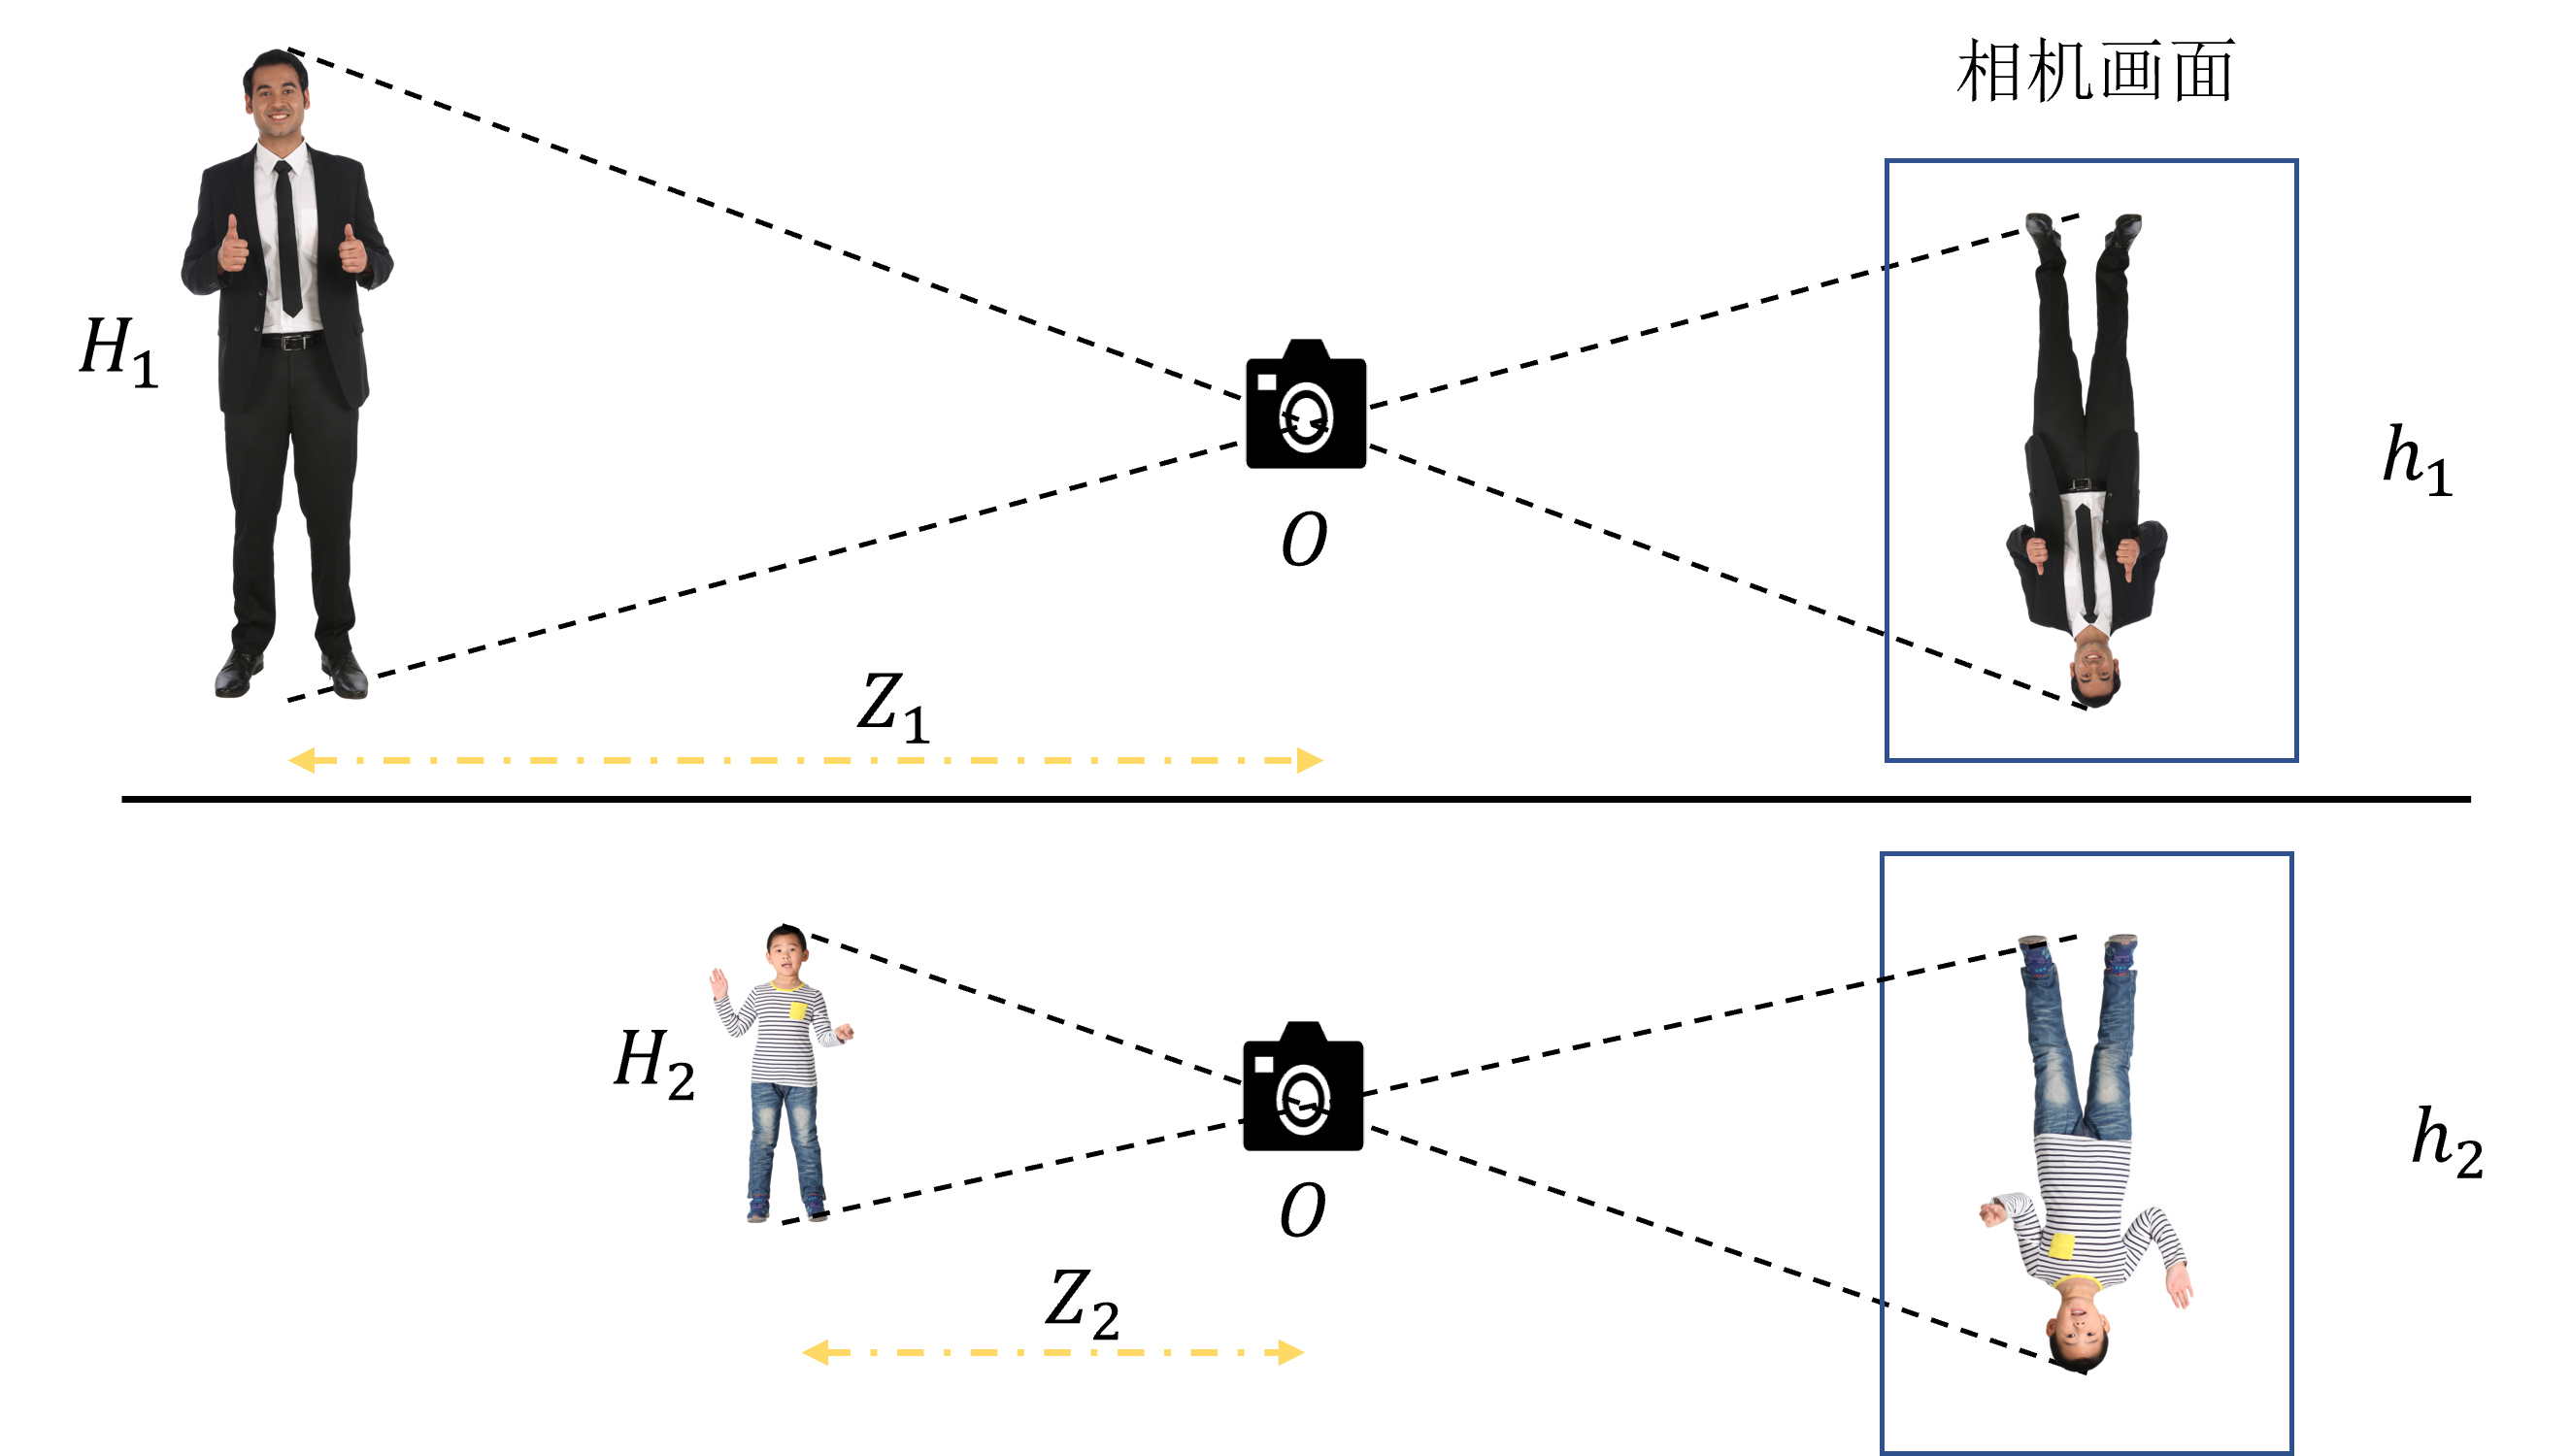
\includegraphics[width=0.75\textwidth]{images/mono_scale_ambiguity.png}
  \caption{单目三维人体姿态估计的尺度模糊示意图}
  \label{fig:mono_scale_ambiguity}
\end{figure}

如图\ref{fig:mono_scale_ambiguity}所示，单目观测只提供视线方向约束：同一像素对应的三维点可以位于该视线上的任意位置。以人体身高为例，在针孔模型下人体在图像中的像素高度$h$与真实身高$H$、距相机的深度$Z$近似满足$h\propto \frac{fH}{Z}$。因此，当观测到相同的投影高度$h$时，不同身高的个体对应不同的真实深度$Z$，仅凭单目图像难以恢复绝对距离与米制尺度。为获得具有物理意义且更稳定的深度线索，本章进一步引入双目立体几何约束，利用视差与三角测量从根源上缓解单目尺度模糊带来的不确定性。

\subsubsection{多目人体姿态估计的问题}
多目三维人体姿态估计常见于动作捕捉棚、智能教室、固定式安防与多机位拍摄等场景：在$V\ge 3$个相机视角下同时观测同一人体，通过跨视角几何约束恢复关节三维坐标，如图~\ref{fig:multi_view_scene} 所示。多目系统能够显著提升可见性并缓解遮挡，因此在受控环境中可获得较高的三维姿态精度与稳定性。

\begin{figure}[htbp]
  \centering
  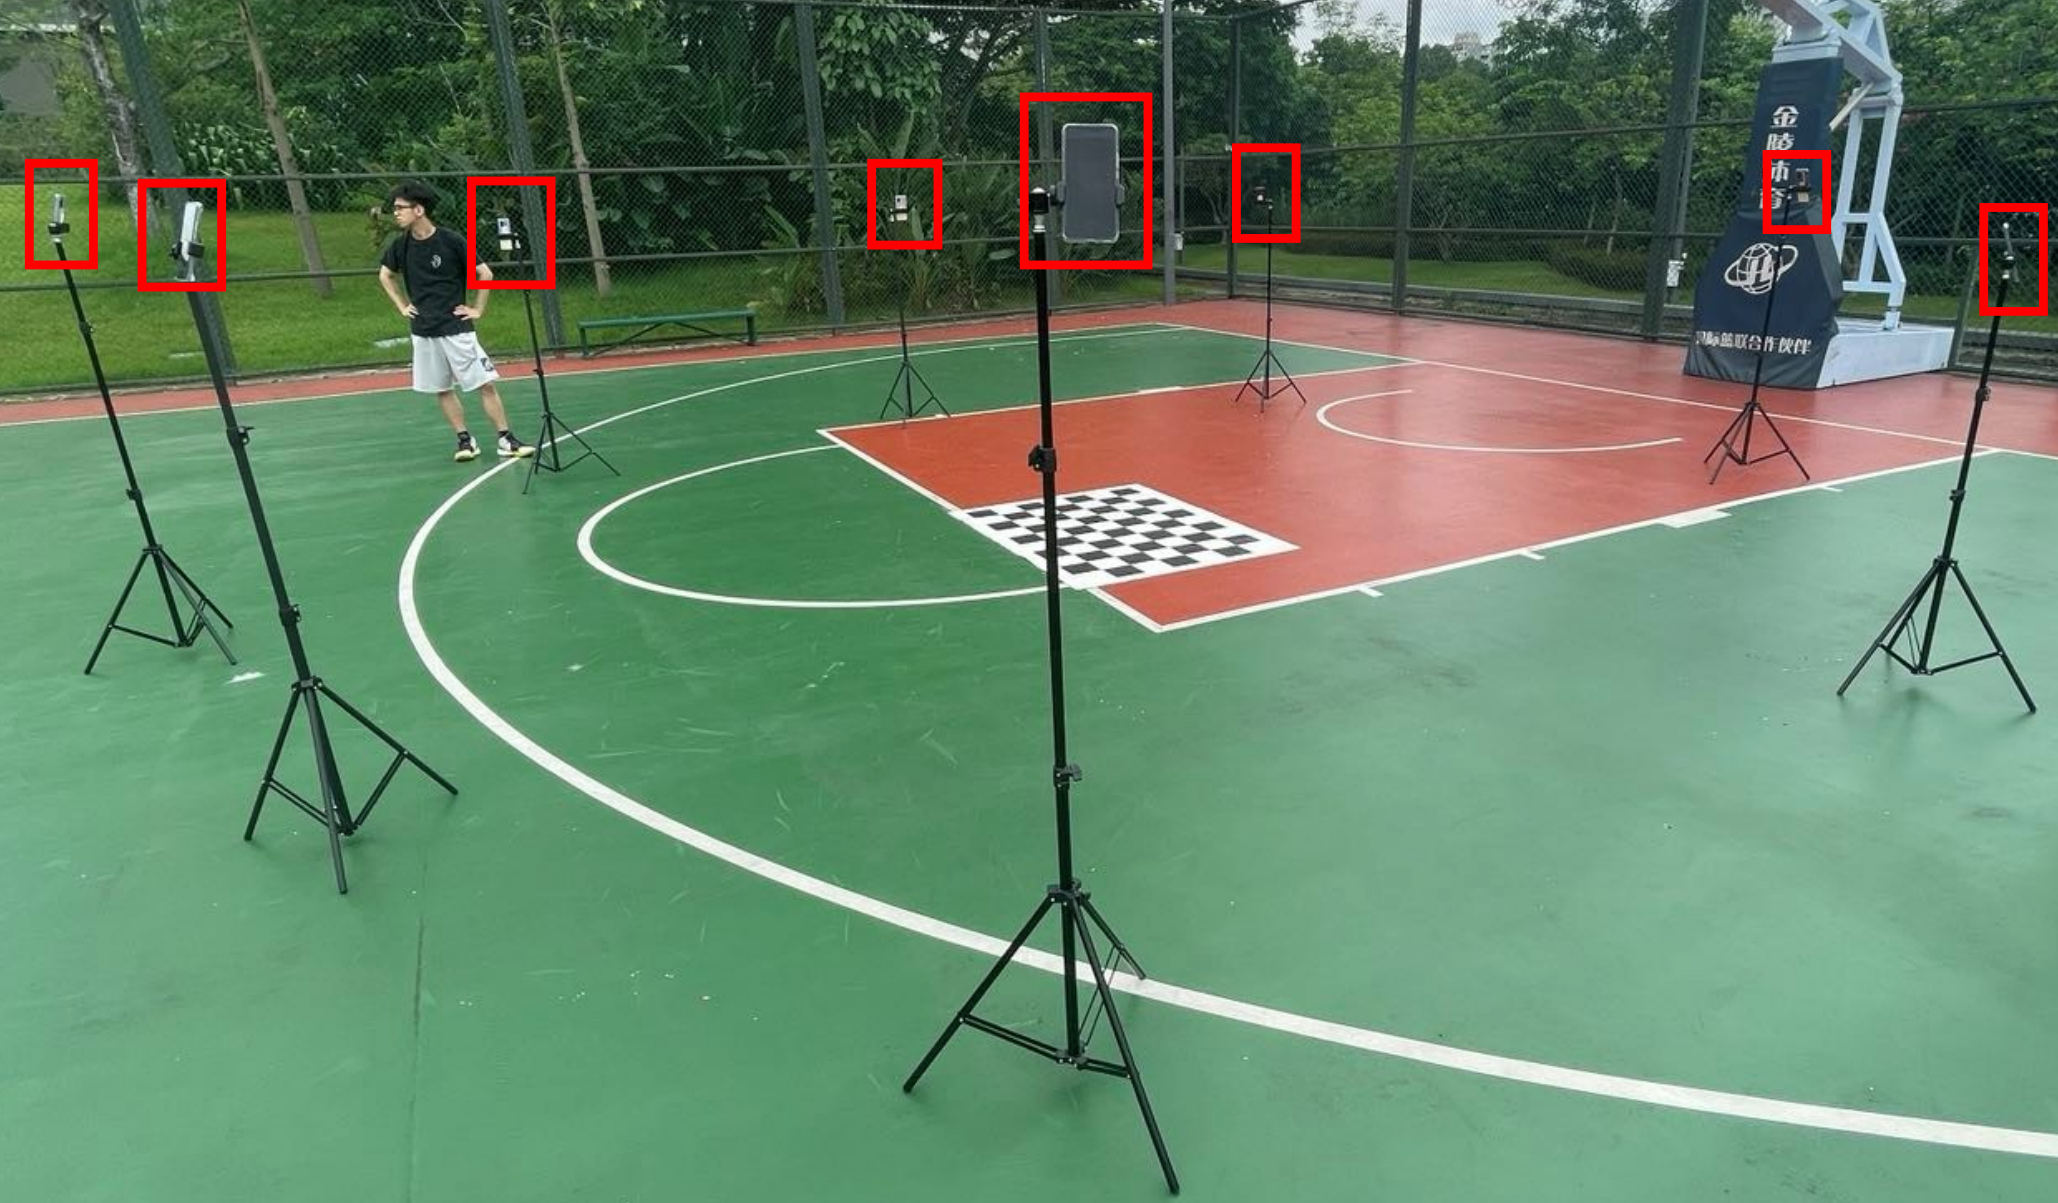
\includegraphics[width=0.85\textwidth]{images/muti_view.png}
  \caption{多视角多相机场景示意图}
  \label{fig:multi_view_scene}
\end{figure}
然而，多目系统的优势往往建立在较高的工程代价之上。在硬件层面，相机数量增加会显著抬升传感器成本与安装复杂度，并对时间同步、标定维护与带宽传输提出更高要求：以常见的4相机动捕系统为例，其单次标定流程通常需要专业人员操作，且标定精度随设备老化和环境变化而退化，难以在消费级场景中持续维护。在计算层面，多视图特征融合与跨视角实例关联的计算量随相机数$V$近似线性增长；在多人在线应用中，跨视角的实例一致性维护与异常观测处理也会引入额外系统开销，使端侧时延更难稳定控制。以 VoxelPose~\cite{tu2020voxelpose} 等具有代表性的多目方法为例，其在4相机配置下仅骨干特征提取部分的 FLOPs 即超过单目方法的3倍，加之视角融合与三维体素化步骤，完整推理链路在移动端 SoC 上难以实现实时运行。在部署层面，固定多相机阵列与端侧移动平台的安装适配性存在先天矛盾，限制了多目系统在服务机器人、可穿戴设备等移动场景中的应用空间。因此，本文选择以双目立体几何为基础，在获得绝对尺度线索的同时，将硬件复杂度与跨视图计算控制在更可落地的范围内。

\subsubsection{现有基于双目人体姿态估计的问题}
前两节分别说明了单目方法存在尺度歧义，多目方法又面临较高的硬件与部署成本，因此双目立体几何构成了更具工程可行性的折中方案。然而，传感器选择上的合理性并不意味着现有双目人体姿态估计方法已经天然适合端侧多人场景。若直接沿用现有双目范式，其推理链路中仍存在明显的计算冗余、模块级串联开销与误差传播风险，难以同时满足“多人、实时、可部署”的要求。

从部署角度看，现有双目人体姿态估计方法的瓶颈主要集中在两条典型技术路径上：一类方法先恢复全图稠密深度，再结合二维关键点反投影得到三维姿态；另一类方法虽然直接在双目特征上进行融合或匹配，但往往保留左右对称的双分支重型骨干。前者的问题在于计算主要消耗在与关节无关的大量像素上，并且误差会沿“深度估计-二维定位-三维反投影”链路逐级累积；后者的问题在于左右视图信息高度相关，却仍以近似双倍的前向代价重复提取表征。基于这一观察，本文将现有方法的端侧瓶颈归纳为以下两类问题：

（1）问题A：基于稠密深度先验的级联范式中，稠密无效像素主导的计算开销与误差累积。

（2）问题B：基于左右对称双分支结构中，跨视图冗余计算与端侧效率瓶颈。

{\bfseries 问题A：基于稠密深度先验的级联范式中，稠密无效像素主导的计算开销与误差累积}\par
一种直观的双目三维人体姿态估计思路是采用“深度先验 + 2D姿态”的级联流程：首先利用双目深度估计网络或立体匹配算法获得整幅图像的稠密视差/深度图$\hat{d}(\mathbf{p})$/$\hat{Z}(\mathbf{p})$，随后采用单目2D人体姿态估计器得到关节像素坐标$\hat{\mathbf{p}}_k=[\hat{u}_k,\hat{v}_k]^\top$，最后在关节处采样深度并通过反投影得到三维关节位置。该范式的核心矛盾在于：深度估计以像素为单位输出整幅图像的稠密深度/视差，而三维人体姿态最终只需在少量关节位置获取深度信息，因而端侧推理开销容易被大量与关节无关的“无效像素”主导，并在两阶段串联中累积误差。
该两阶段级联流程如图~\ref{fig:two_stage_dualocular_pipeline}所示。

\begin{figure}[htbp]
  \centering
  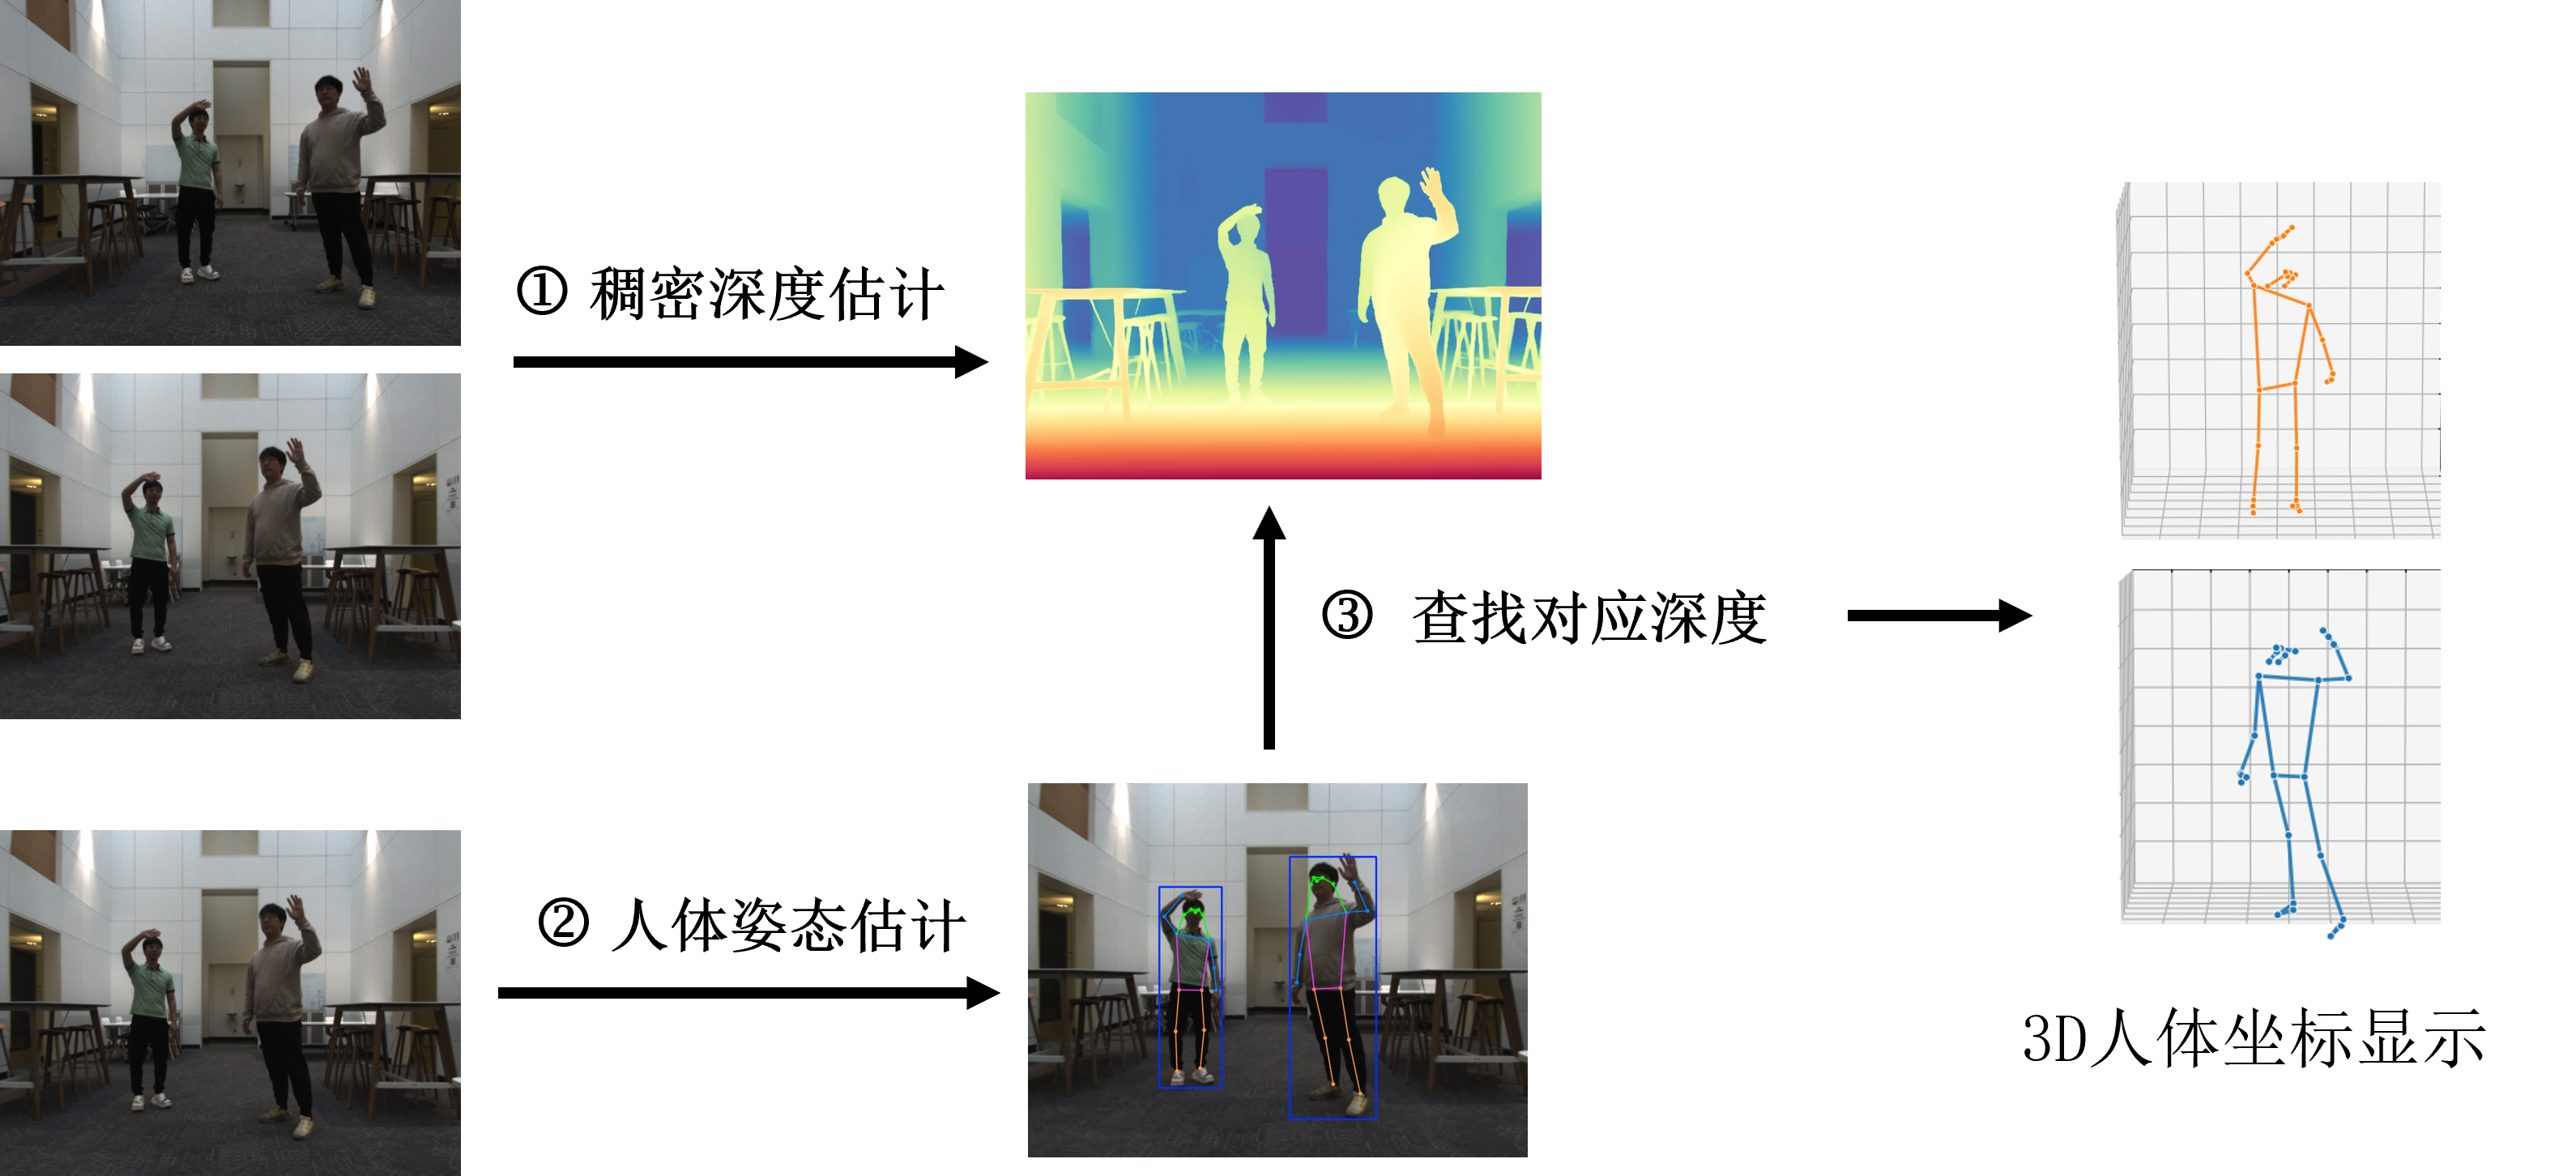
\includegraphics[width=0.88\textwidth]{images/Two-Stage_Dualocular_Human_Pose_Estimation.png}
  \caption{基于稠密深度先验的双目两阶段三维人体姿态估计流程示意图}
  \label{fig:two_stage_dualocular_pipeline}
\end{figure}

以立体校正后的双目相机为例，设焦距为$f$、基线为$B$，则深度与视差满足
\begin{equation}
\hat{Z}(\mathbf{p})=\frac{fB}{\hat{d}(\mathbf{p})}.
\label{eq:depth_from_disp}
\end{equation}
给定相机内参矩阵$\mathbf{K}$与齐次像素坐标$\tilde{\mathbf{p}}_k=[\hat{u}_k,\hat{v}_k,1]^\top$，对应的三维关节估计可写为
\begin{equation}
\hat{\mathbf{X}}_k = \hat{Z}(\hat{\mathbf{p}}_k)\mathbf{K}^{-1}\tilde{\mathbf{p}}_k .
\label{eq:joint_backproject}
\end{equation}
该流程实现简单，且能够在几何意义上输出具有米制尺度的三维坐标，因此在工程上具有一定吸引力。然而，将稠密深度估计作为前置模块并与2D姿态简单叠加，会在端侧多人场景中暴露出明显的效率与精度问题。

第一，稠密无效像素主导的计算开销。稠密深度估计以像素为单位输出$H\times W$的深度图，并通常需要在较大的视差范围上进行匹配与正则化，其计算与内存开销主要由图像分辨率与视差范围决定，与实际需要的关节数量无关。对于多人姿态任务，最终仅需为每个目标的有限关键点集合$\{\mathbf{p}_k\}_{k=1}^{K}$恢复深度，其中$K$通常为$17$或$24$等常数。若直接计算全图深度，再对少量关键点采样，则大量像素的匹配计算不会对最终三维关节精度产生直接贡献，导致端侧推理时延与功耗被”无效像素”主导；当输入分辨率提高以满足2D关键点定位需求时，该冗余将进一步放大。此外，在端侧部署中，稠密深度网络与2D姿态网络通常各自包含多尺度特征提取、上下采样与后处理模块，简单串联会导致参数量、激活占用与访存带宽叠加；同时，深度图输出到关节深度采样之间还可能需要插值、滤波、置信度筛选与空洞填补等步骤，以缓解离散化与噪声对关节的影响，这些操作会增加不可忽略的CPU/GPU开销并引入额外时延。更重要的是，该级联结构无法充分共享双目两视图的中间特征表示，使得跨视图信息在深度阶段与姿态阶段被重复建模，进一步降低整体能效比。

第二，级联结构的误差累积。由式\eqref{eq:depth_from_disp}可知，当视差估计存在误差$\delta d$时，深度误差近似满足
\begin{equation}
\delta Z \approx \left|\frac{\partial Z}{\partial d}\right|\delta d = \frac{fB}{d^2}\delta d,
\label{eq:depth_error_propagation}
\end{equation}
这意味着在远距离（小视差）区域，亚像素级视差误差也会被放大为较大的深度波动。进一步代入式\eqref{eq:joint_backproject}，三维关节误差由深度误差与像素定位误差共同决定：一方面，2D关键点在遮挡、运动模糊和弱纹理条件下易产生抖动，使得采样位置落入深度图的误匹配区域或深度不连续边缘；另一方面，深度网络的优化目标通常是像素级重投影误差或视差回归损失，其最优解并不必然在人体关节区域具有最小误差，尤其在衣物褶皱、细肢体结构和自遮挡处，深度图可能出现孔洞、飞点（flying pixels）或边界泄漏，从而导致关节深度在时间上产生跳变。由于级联方法缺乏从”关节三维误差”到”深度估计”的端到端反馈，系统难以针对关键点区域进行定向纠错，三维姿态往往呈现对场景与成像条件敏感的非平滑行为。

{\bfseries 问题B：基于左右对称双分支结构的跨视图冗余计算与端侧效率瓶颈}\par
在网络结构上，许多双目姿态方法采用左右对称的双分支骨干分别提取特征，再进行融合或匹配。该左右对称双分支结构的典型流程如图~\ref{fig:symmetric_dual_branch_pipeline} 所示。这种设计虽然直观，且左右分支通常共享网络权重以减少参数量，但权重共享仅意味着模型存储开销不变，实际推理时仍需对左右两幅图像分别执行一次完整的前向传播，因此骨干网络与多尺度融合模块的计算量（FLOPs）与激活显存占用仍然近似翻倍，并引入大量跨视图冗余表征。在多人场景中，若后续还需进行实例级关联或多阶段细化，则系统开销会进一步叠加，导致端侧实时性不足且时延随场景复杂度波动明显。

\begin{figure}[htbp]
  \centering
  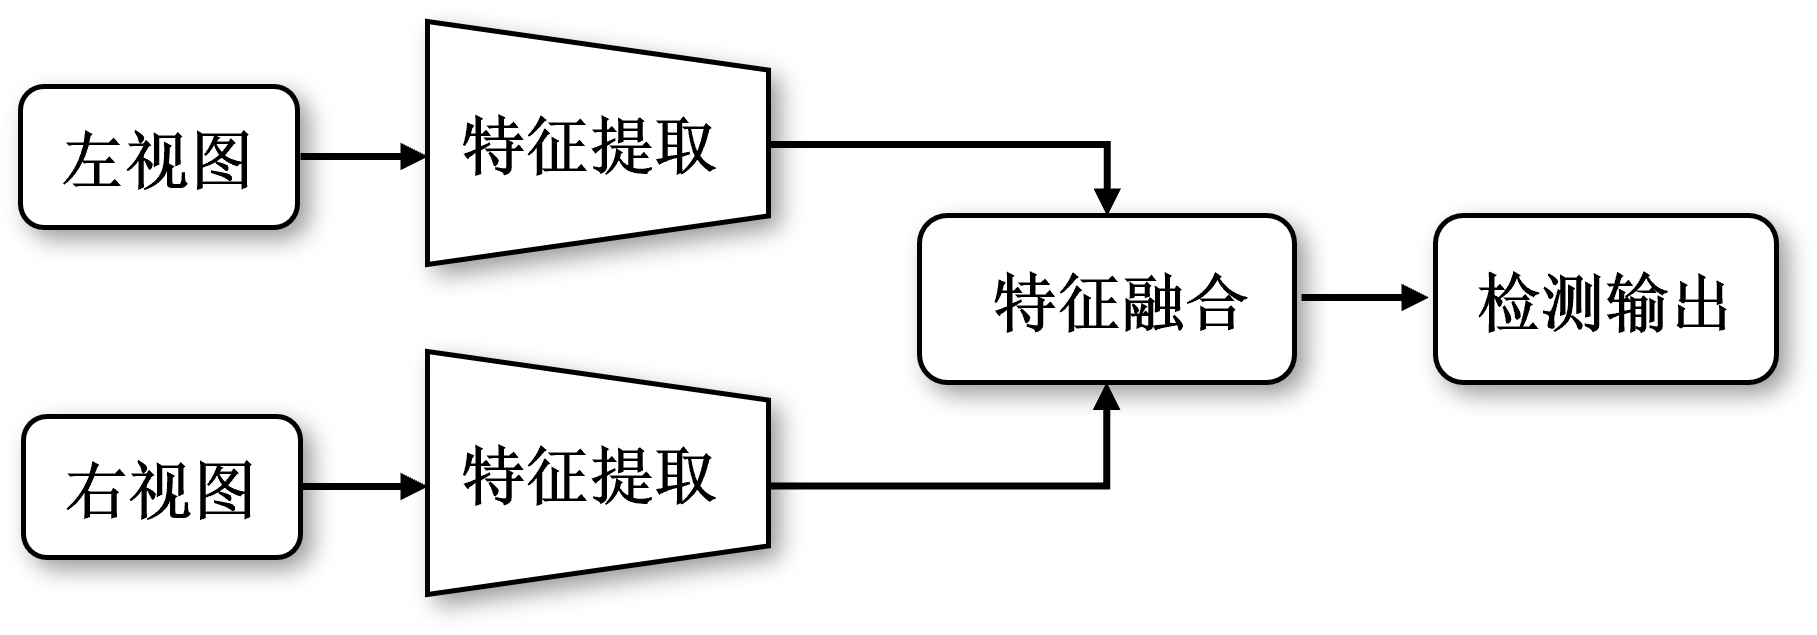
\includegraphics[width=0.80\textwidth]{images/Left_and_right_symmetrical_double_branch_structure.png}
  \caption{基于左右对称双分支结构的双目人体姿态估计流程示意图}
  \label{fig:symmetric_dual_branch_pipeline}
\end{figure}

为直观评估”左右视图内容高度相似”所带来的冗余，我们将同一双目输入分别送入全量 CSPDarknet 骨干，提取关键点热力图，结果如图~\ref{fig:stereo_heatmap_redundancy} 所示：左右视图的响应分布与峰值位置高度重叠，说明两套全量骨干在信息增益上非常有限，却会带来近乎两倍的参数量与 FLOPs，显著挤占端侧算力与内存带宽。这一可视化证据为后续左重右轻的非对称设计提供了直接动机。

\begin{figure}[htbp]
  \centering
  \begin{subfigure}[t]{0.47\textwidth}
    \centering
    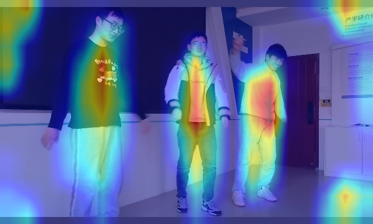
\includegraphics[width=\textwidth]{images/Left_perspective_heatmap_visualization.png}
    \caption{左视图热力图}
  \end{subfigure}\hfill
  \begin{subfigure}[t]{0.47\textwidth}
    \centering
    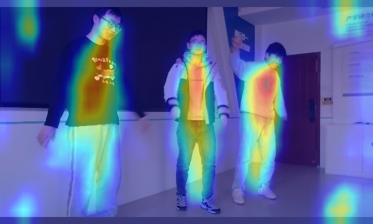
\includegraphics[width=\textwidth]{images/Right_perspective_heatmap_visualization.png}
    \caption{右视图热力图}
  \end{subfigure}
\caption{左右视图热力图对比}
  \label{fig:stereo_heatmap_redundancy}
\end{figure}


综合上述分析可以看出，现有双目方法的主要困难并不在于“双目几何是否有效”，而在于其常见实现路径仍然延续了稠密视觉任务或对称网络设计的计算习惯，没有围绕“三维关节恢复”这一目标重新组织推理链路。由此，本章后续方法设计的基本思路是：以关节任务为中心组织双目特征交互与三维恢复，跳过全图稠密深度中间表示，削减左右对称结构中的重复计算，从而构建轻量且几何可解释的端侧推理链路。

\paragraph{设计依据与方法动机}
对于双目三维人体姿态估计，目标并不是对左右视图分别完成一套对等的三维理解，而是围绕同一组人体关节完成二维定位、跨视图对应与三维恢复。就这一任务链路而言，一个视图首先需要提供稳定的二维关节位置与人体结构表征，作为后续几何恢复的参考；另一视图的主要作用则是围绕这些已定位关节提供跨视图匹配线索，以确定视差并支撑三角化求解。由于高精度定位更依赖空间分辨率和语义表达能力，而匹配过程更关注跨视图的一致性与局部相关性，因此两个分支在任务中的作用并不对等，也没有必要配置完全相同的计算资源。这种功能分工也可类比为人类双眼视觉中的主导眼与辅眼协同：前者更侧重稳定的空间参照，后者提供补充的视差信息，但二者并不意味着需要完全对等的信息处理负担。

从信息冗余角度看，左右视图本质上是同一物理空间的两次相近投影，二者之间具有较高互信息。若在两个分支中同时部署重型骨干网络提取深层特征，虽然结构上直观，但在端侧计算代价上并不经济。非对称设计正是基于这一点：主分支保留更强的几何与语义表征能力，轻量化分支则尽可能压缩冗余描述，仅保留跨视图匹配所需的基础纹理与几何线索，从而在不破坏双目匹配有效性的前提下，将有限算力集中到对三维恢复更关键的表征上。

基于上述设计依据，本文围绕“关节级跨视图匹配与三维恢复”这一核心任务，从骨干架构、跨视图交互、三维求解与训练约束四个层面构建轻量化非对称双目学习框架：以非对称骨干压缩左右分支冗余，以 EFEM 建立受极线约束的低开销跨视图匹配，以可微加权三角化求解器实现端到端三维恢复，再以跨分支一致性约束弥补轻量分支的表示能力损失。通过这一设计，本章在不构建全图稠密深度或高维代价体的前提下，将有限计算资源集中于对三维关键点最敏感的区域与表征上，从而在精度与效率之间取得更适配端侧部署的平衡。

\subsection{轻量化非对称双目学习框架与网络结构设计}

针对 3.2 节归纳的两类瓶颈——稠密级联开销（问题A）与左右对称冗余（问题B）——本节提出轻量化非对称双目学习框架。其核心设计由四个相互协同的模块构成：非对称双目骨干网络（第~\ref{subsubsec:asym_backbone}节）、极线特征增强模块（第~\ref{subsubsec:efem}节）、可微加权三角化姿态求解器（第~\ref{subsubsec:dwt}节）与跨分支表征一致性约束（第~\ref{subsubsec:align_loss}节）。这四个模块并非简单并列堆叠，而是按“先压缩冗余表征、再增强跨视图几何、继而完成可微三维恢复、最后补偿轻量分支能力”的逻辑逐步展开。

\subsubsection{整体框架与端到端流程}
\label{subsubsec:overall_pipeline}
针对 3.2.3 节总结的稠密级联开销与左右对称冗余等问题，本文提出轻量化双目三维人体姿态估计框架，其整体流程如图~\ref{fig:pipeline_ch3} 所示。该框架在端侧场景中同时兼顾几何精度与实时性，以“关节任务为中心”组织双目特征交互与三维恢复：输入为立体校正后的左右视图，首先经非对称双目骨干网络提取多尺度特征金字塔$\{\mathbf{F}^l_s\}$与$\{\mathbf{F}^r_s\}$；随后在主尺度特征上引入极线特征增强模块，在极线约束下将跨视图匹配从二维搜索降为一维视差窗口搜索，并以右分支特征作为查询、左分支特征作为键和值完成交叉注意力聚合，从而向右分支注入几何一致性信息并得到增强表征；在此基础上，通过可微加权三角化姿态求解器将左右视图的二维观测与相机模型融合为三维关节坐标；训练阶段再联合跨分支表征一致性约束，使轻量分支在不增加推理开销的前提下获得更强的几何感知能力。

\begin{figure}[htbp]
  \centering
  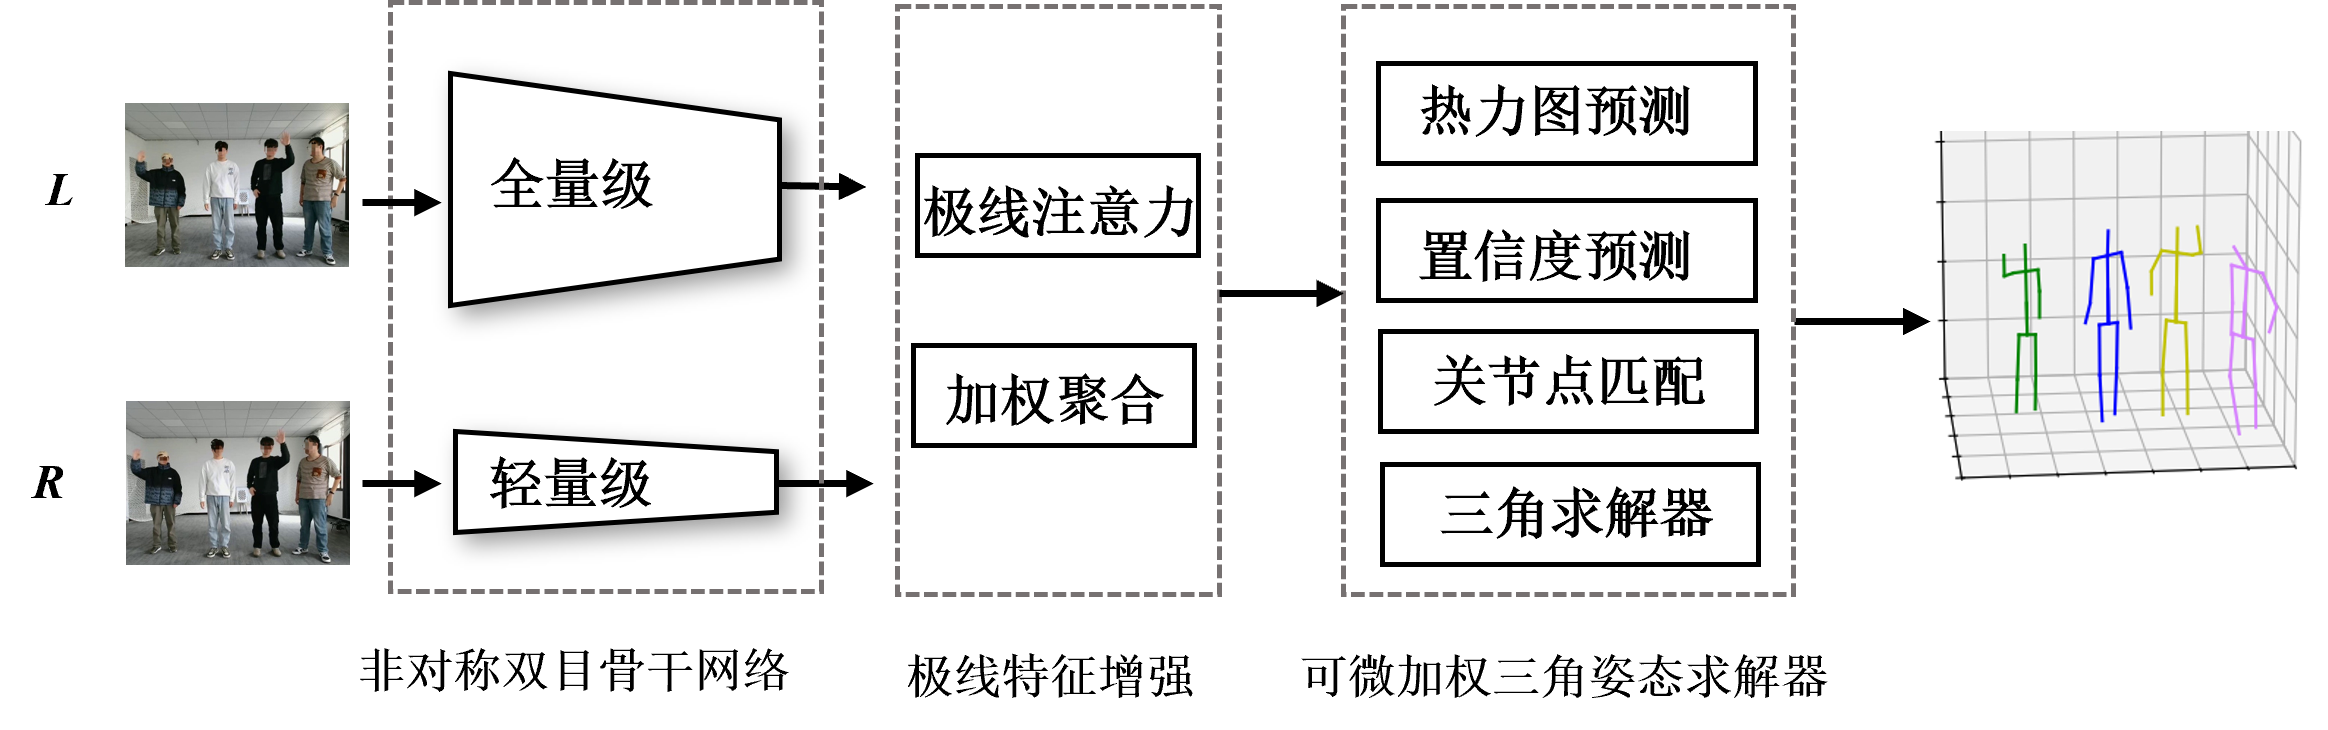
\includegraphics[width=0.95\textwidth]{images/Pipline.png}
  \caption{本文轻量化非对称双目三维人体姿态估计框架整体流程图}
  \label{fig:pipeline_ch3}
\end{figure}

从多人姿态检测的范式来看，本文采用自底向上的整图推理链路：在整幅图像上一次性预测多人关键点热力图并完成关节级几何求解，从而避免自顶向下方法“按人裁剪、逐实例回归”带来的人数相关循环开销。其端到端计算开销主要由像素级骨干网络前向决定，复杂度近似为$\mathcal{O}(HW)$；而三维求解器仅在稀疏的$M\times J$关节特征上运行（$M$为人数，$J=17$为常数），复杂度为$\mathcal{O}(MJ)$，因此在多人场景下具有更稳定的时延表现。

\paragraph{多人实例构建与二维关键点解码}
为将整图预测结果转化为逐人的二维关键点观测，本文采用中心点引导的自底向上解码策略：二维预测头除输出各关节热力图外，还预测人体中心热力图；推理阶段先在中心热力图上结合非极大值抑制得到各实例中心，再由回归分支恢复各关节相对中心的偏移，从而获得逐实例二维关键点观测。由于左右视图独立检测，检测到的人数与实例顺序可能不一致，因此在三角化之前需要建立跨视图实例关联；本文利用立体校正后的极线约束，在右视图对应水平扫描线附近搜索候选中心，并采用贪心匹配建立左右实例的一一对应关系，未匹配成功的实例不参与后续三角化。最终，匹配后的左右二维观测$\mathbf{x}_{l,m,j}$与$\mathbf{x}_{r,m,j}$被送入第~\ref{subsubsec:dwt}节的可微加权三角化姿态求解器，得到三维关节$\hat{\mathbf{X}}_{m,j}$；后续推导为简洁起见省略实例下标$m$，但实现中仍对每个实例独立求解。

\subsubsection{非对称双目骨干网络设计}
\label{subsubsec:asym_backbone}
该模块对应整条方法链的第一步：在进入跨视图交互之前，先尽可能压缩左右分支的重复表征开销，同时保留支撑后续匹配与三维恢复所需的主干语义与几何信息。
如图~\ref{fig:stereo_heatmap_redundancy} 所示，左右视图在高容量骨干下的响应分布高度重叠，说明“左右各一套全量骨干”的信息增益有限而计算冗余显著。基于此，本文采用“左重右轻”的非对称双分支骨干网络：左分支使用高容量 CSPDarknet 骨干提取高保真语义与几何特征，右分支采用结构同构的轻量化骨干，在保持算子类型与特征层级对齐的前提下，将通道宽度缩减为全量分支的 $0.5$ 倍（width\_multiple=0.5），并将深度缩减为全量分支的 $0.34$ 倍（depth\_multiple=0.34）。据此，右分支骨干的参数量与 FLOPs 可压缩至全量分支骨干的约 $40\%$；结合预测头等共享模块后，非对称方案的整体参数量与 FLOPs 分别约为对称全量方案的 $62\%$（详见表~\ref{tab:ablation_asym_stereo}）。两分支各阶段输出通道配置见表~\ref{tab:backbone_config}。

\begin{table}[htbp]
  \centering
  \small
\caption{非对称双目骨干网络通道配置对比}
  \label{tab:backbone_config}
  \begin{tabular}{lcccc}
    \toprule
    分支 & 步幅$s=8$ & 步幅$s=16$ & 步幅$s=32$ & width\_multiple \\
    \midrule
    左分支（全量，CSPDarknet-M） & 256 & 512 & 1024 & 1.0 \\
    右分支（轻量，CSPDarknet-N） & 128 & 256 & 512  & 0.5 \\
    \bottomrule
  \end{tabular}
\end{table}

图~\ref{fig:cspdarknet_arch} 展示了非对称双目骨干网络的整体结构与单个 CSP Block 的内部展开。两分支均以 Stem 层完成初始下采样（$\times4$），随后依次经过 P3、P4、P5 三个阶段提取多尺度特征；每个 CSP Block 均采用“一路直传 + 一路 Bottleneck 堆叠”的双路结构，在保持表征多样性的同时减少重复计算。

\begin{figure}[htbp]
  \centering
  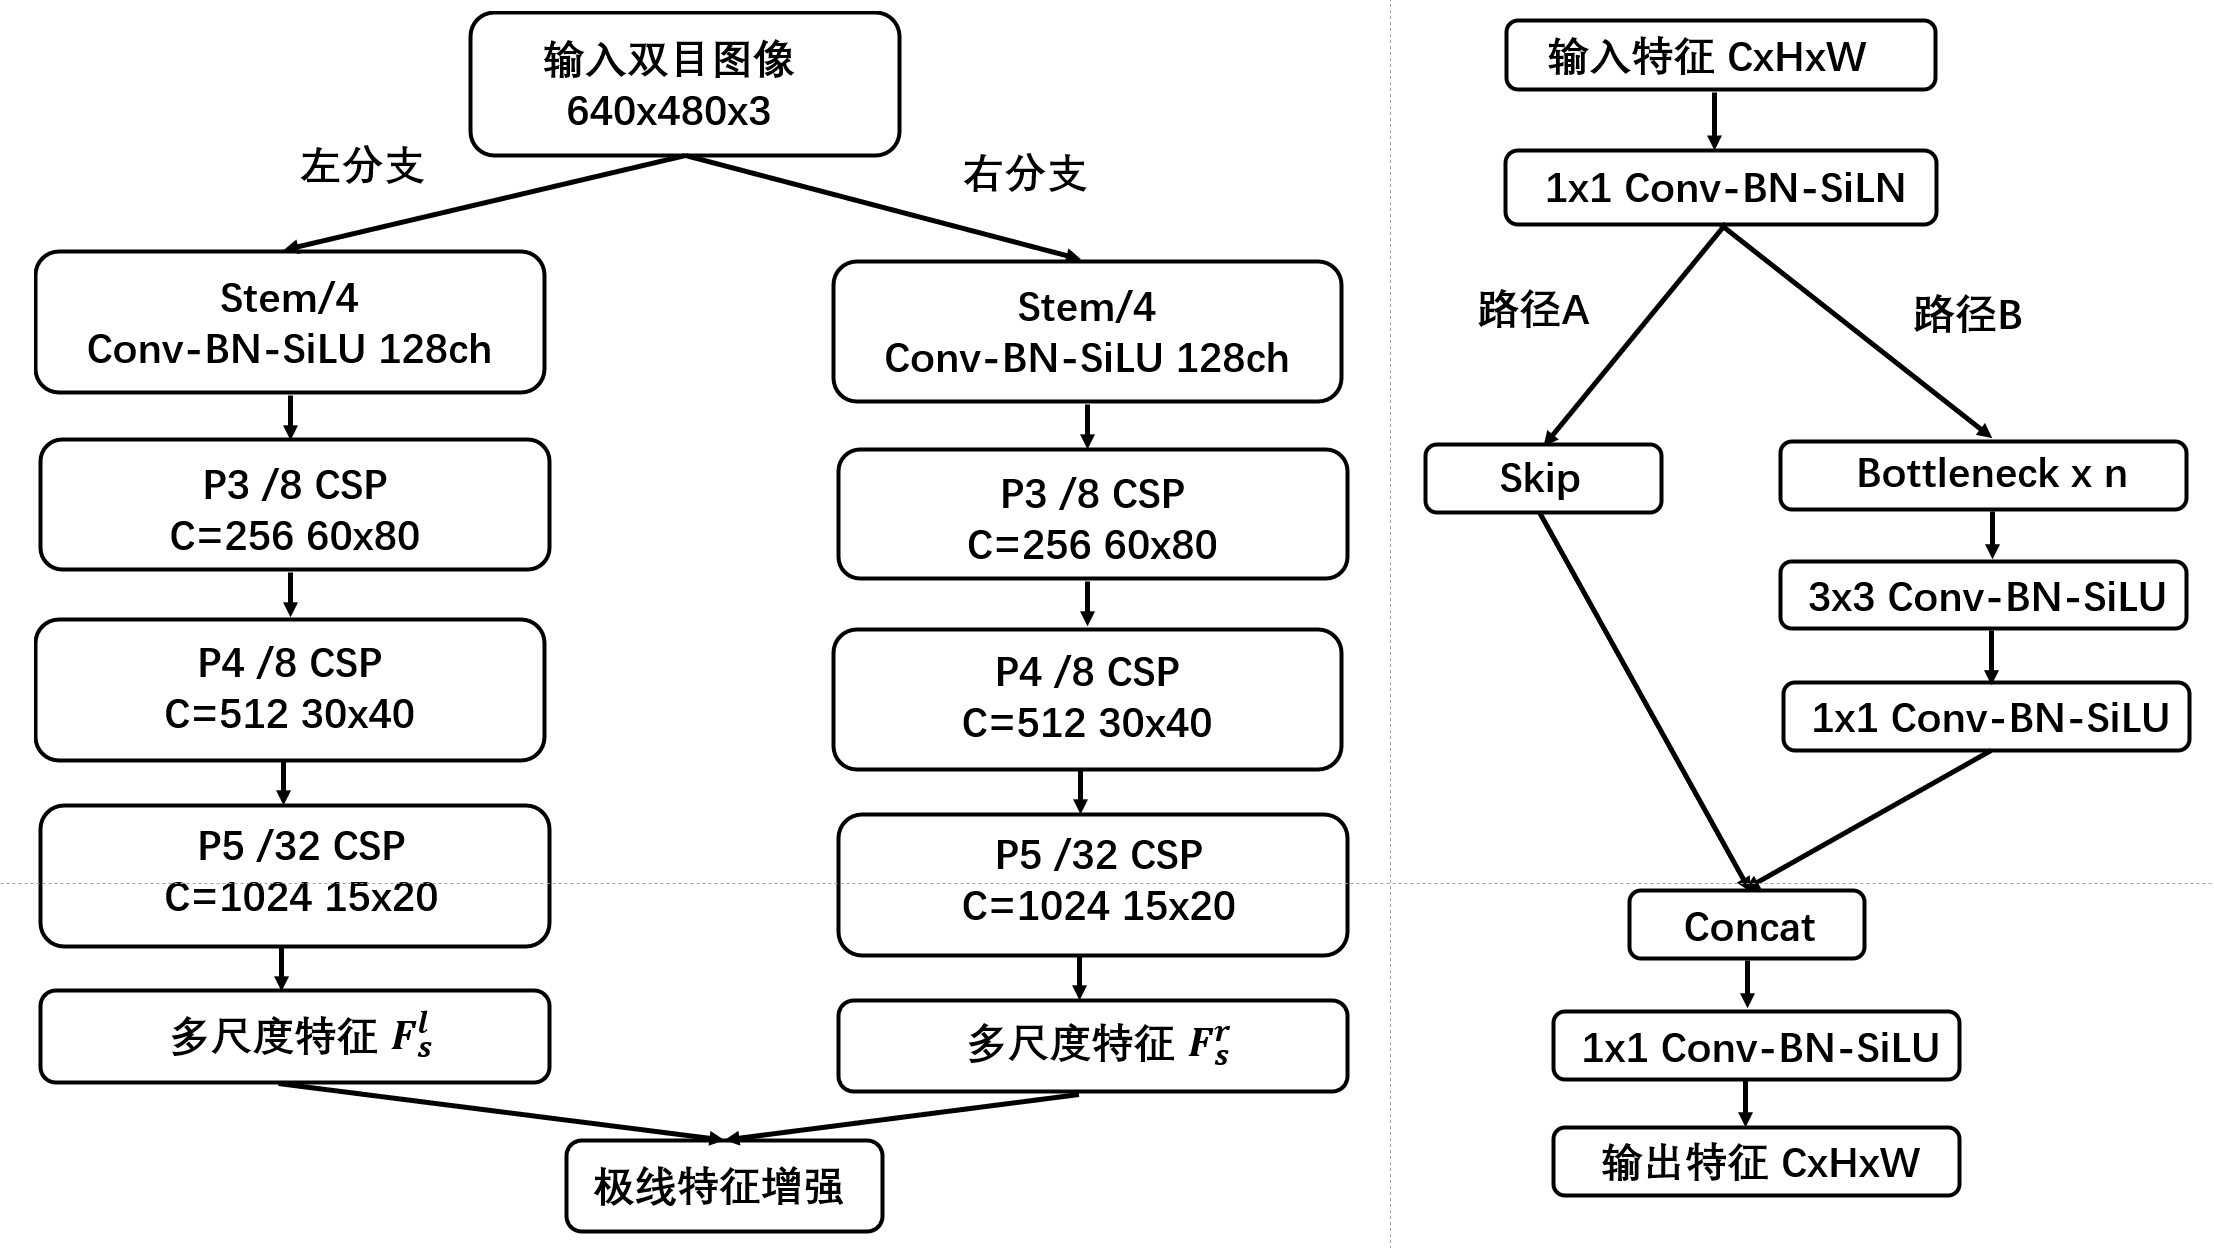
\includegraphics[width=\textwidth]{images/Overall_structure_of_asymmetric_binocular_backbone_network}
  \caption{非对称双目骨干网络结构示意图}
  \label{fig:cspdarknet_arch}
\end{figure}

在几何层面，哪一侧作为全量分支、哪一侧作为轻量分支并无本质区别，左右可以互换。本文固定左分支为全量分支，主要是为了与后续 EFEM 中“右作查询、左作键值”的跨视图交互方式保持一致；训练阶段再引入跨分支表征一致性约束，以缩小轻量分支与全量分支之间的表示差距。

\subsubsection{极线特征增强模块}
\label{subsubsec:efem}
\paragraph{设计目标与总体思路}
在骨干层面压缩冗余之后，下一步需要回答的问题是：如何在不恢复到稠密代价体建模的前提下，为轻量右分支补足稳定的跨视图几何线索。极线特征增强模块的核心目标正是：在不构建高维代价体的前提下，沿极线方向建立低开销的跨视图注意力，显式增强与关键点相关的几何一致性。为避免全图匹配与对称重复计算，EFEM 以右视图特征作为查询、左视图特征作为键和值，把跨视图交互约束在水平扫描线上，通过一维注意力将左视图的几何一致性信息注入右分支表征，为后续三维求解提供更具判别性的输入。

\begin{figure}[htbp]
  \centering
  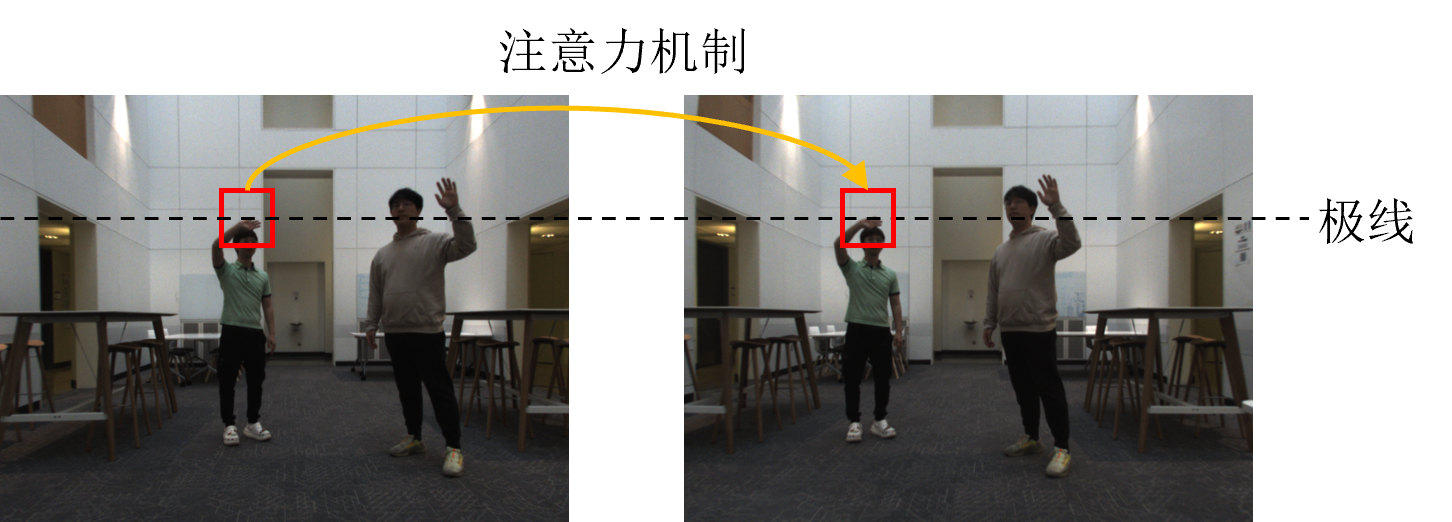
\includegraphics[width=0.88\textwidth]{images/crossattention.png}
\caption{极线交叉注意力计算示意图}
  \label{fig:efem_crossattention}
\end{figure}

\paragraph{输入压缩与查询-键构建}
设左右分支特征为$\mathbf{F}_l,\mathbf{F}_r\in\mathbb{R}^{C\times H\times W}$。EFEM 以右分支当前位置为锚点沿极线发起匹配，并以左分支特征作为可检索的跨视图记忆。为构造沿极线的交叉注意力，先通过轻量投影得到查询、键和值：
\begin{equation}
\mathbf{q}=\phi_q(\mathbf{F}_r),\quad \mathbf{k}=\phi_k(\mathbf{F}_l),\quad \mathbf{v}=\phi_v(\mathbf{F}_l),\quad \mathbf{q},\mathbf{k},\mathbf{v}\in\mathbb{R}^{C'\times H\times W},
\label{eq:efem_proj}
\end{equation}
其中$\phi_q,\phi_k,\phi_v$为$1\times1$卷积+归一化（可选分组卷积），分别将右分支特征映射为查询向量，并将左分支特征映射为键和值，以在控制计算开销的同时对齐跨视图表征维度。

\paragraph{极线注意力与加权聚合}
在立体校正条件下，搜索限定在同一行$y=v$的视差窗口$\mathcal{D}=\{0,\ldots,D-1\}$。此处$d\geq0$表示左视图特征相对于右视图特征在水平方向上的正向偏移，与标准双目约定（视差$d=u_l-u_r\geq0$，即同一物点在左图中的横坐标不小于在右图中的横坐标）一致，在特征图坐标下同样成立。对每个位置$(u,v)$计算右视图查询$\mathbf{q}(u,v)$与左视图键$\mathbf{k}(u+d,v)$的相关分数：
\begin{equation}
s(u,v,d)=\frac{\langle \mathbf{q}(u,v),\mathbf{k}(u+d,v)\rangle}{\sqrt{C'}},\quad d\in\mathcal{D},
\label{eq:efem_score}
\end{equation}
并在视差维做 softmax 得到注意力权重
\begin{equation}
\alpha(u,v,d)=\frac{\exp(s(u,v,d))}{\sum_{d'\in\mathcal{D}}\exp(s(u,v,d'))}.
\label{eq:efem_weight}
\end{equation}
利用注意力权重对左视图的值向量$\mathbf{v}$加权聚合，得到与$(u,v)$对齐的几何增强向量
\begin{equation}
\mathbf{g}(u,v)=\sum_{d\in\mathcal{D}}\alpha(u,v,d)\mathbf{v}(u+d,v).
\label{eq:efem_agg}
\end{equation}

\begin{figure}[htbp]
  \centering
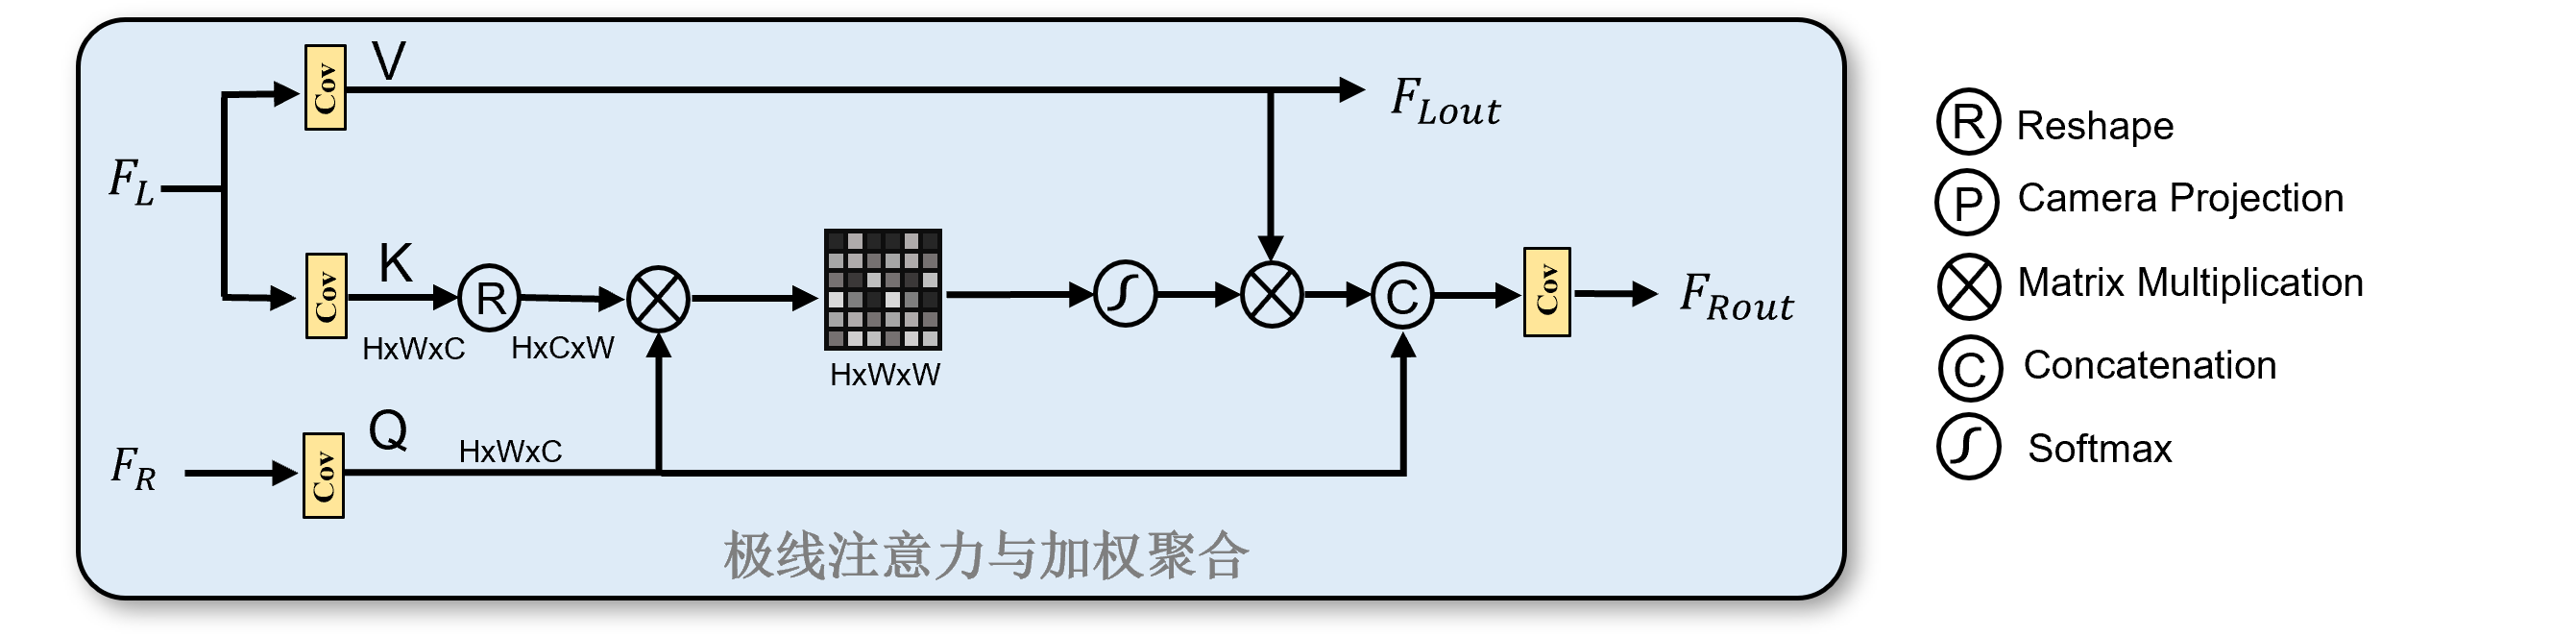
\includegraphics[width=0.92\textwidth]{images/Epipolar_attention_and_weighted_aggregation.png}
\caption{极线注意力与加权聚合过程示意图}
\label{fig:efem_epipolar_weighted_aggregation}
\end{figure}
再与右视图局部特征融合输出
\begin{equation}
\hat{\mathbf{q}}=\psi\!\left([\mathbf{q},\mathbf{g}]\right),
\label{eq:efem_fuse}
\end{equation}
其中$\psi(\cdot)$为$1\times1$卷积，用于融合右视图局部语义$\mathbf{q}$与沿极线聚合得到的几何增强向量$\mathbf{g}$，输出供后续模块使用的增强特征$\hat{\mathbf{q}}$。

\paragraph{复杂度分析与端侧友好性}
在默认全宽搜索时，复杂度为$\mathcal{O}(H\,W^{2}C')$；若根据场景设定最大视差$D_{\max}$，则可裁剪为$\mathcal{O}(H\,W\,D_{\max}C')$，更适合移动 SoC/NPU 上的确定时延执行。EFEM 输出的$\hat{\mathbf{q}}$携带沿极线聚合得到的跨视图一致性信息，可为后续三维求解提供更稳定的关节相关表征，从而在不构建代价体的情况下提升双目几何推断的稳定性。
\subsubsection{可微加权三角化姿态求解器}
\label{subsubsec:dwt}
在获得跨视图增强后的二维表征之后，方法链的第三步是把双视图观测稳定地转化为三维监督信号。可微加权三角化姿态求解器的核心目标是：在双目视图条件下，将左/右视图的二维关键点观测与相机模型融合为三维关节坐标，并在深度学习框架中保持端到端可训练性。为此，本节将传统双目三角化改写为可微的加权最小二乘问题，并引入由特征图预测的视图置信度权重，以增强在遮挡与误检情况下的鲁棒性。

\paragraph{设计目标与总体思路}
在深度学习框架下直接使用传统三角化存在两个关键问题：其一，二维关键点检测存在噪声，遮挡、模糊或复杂姿态会带来较大误差；其二，若通过$\arg\max$从热力图提取二维坐标，则三维监督信号无法反向传播至热力图网络。若将热力图峰值位置作为二维观测
\begin{equation}
(u_{c,j},v_{c,j})=\arg\max\limits_{(u,v)\in\Omega} H_{c,j}(u,v),
\label{eq:pdrm_argmax}
\end{equation}
其中$c\in\{l,r\}$表示左/右视图，$H_{c,j}=\phi_h(\mathbf{F}_c)$为由特征图$\mathbf{F}_c$经热力图头$\phi_h(\cdot)$预测得到的关节热力图。由于$(u_{c,j},v_{c,j})$是离散索引，对$H_{c,j}$几乎处处不可导，三维误差难以有效反向更新关键点热力图分布。为此，本文采用三项协同设计：其一，使用软argmax（见式\eqref{eq:pdrm_softarg_u}--\eqref{eq:pdrm_softarg_v}）提取连续二维坐标；其二，为左右视图分配可学习置信度权重；其三，将双目三角化统一为加权最小二乘问题，并通过闭式求解恢复三维点，从而实现端到端训练。
其中，双目条件下反齐次化后的绝对尺度由相机标定参数确定，与第二章所讨论的单目尺度模糊问题不同。

\paragraph{与热力图的可微连接}
首先对热力图进行二维归一化，得到概率分布
\begin{equation}
p_{c,j}(u,v)=\frac{\exp(H_{c,j}(u,v))}{\sum\limits_{(u',v')\in\Omega}\exp(H_{c,j}(u',v'))}
\label{eq:pdrm_softmax2d}
\end{equation}
其中$\Omega$为热力图的离散像素集合。软argmax 对应的二维坐标期望为
\begin{align}
u_{c,j}&=\sum\limits_{(u,v)\in\Omega} u\cdot p_{c,j}(u,v),
\label{eq:pdrm_softarg_u}\\
v_{c,j}&=\sum\limits_{(u,v)\in\Omega} v\cdot p_{c,j}(u,v).
\label{eq:pdrm_softarg_v}
\end{align}
由于 softmax 与加权求和均为可微操作，故$\mathbf{x}_{c,j}$关于热力图$H_{c,j}$可导，从而三维监督损失能够端到端反向传播。本文在此选择 softargmax 而非离散 $\arg\max$，核心并不在于得到“更平滑”的二维坐标本身，而在于保留“热力图分布$\rightarrow$二维观测$\rightarrow$三维误差”的连续梯度链路。训练与推理阶段均采用 softargmax 提取二维坐标，以保持训练-推理的一致性，避免因坐标提取方式不同引入分布偏移。

\paragraph{投影约束与线性化}
设投影矩阵 $\mathbf{P}_c\in\mathbb{R}^{3\times4}$ 的三行分别为
\begin{equation}
\mathbf{P}_c=
\begin{bmatrix}
\mathbf{p}_{1,c}^\top\\
\mathbf{p}_{2,c}^\top\\
\mathbf{p}_{3,c}^\top
\end{bmatrix}.
\label{eq:pdrm_P_rows}
\end{equation}
根据透视投影模型，在齐次坐标下有
\begin{equation}
\tilde{\mathbf{x}}_{c,j}\sim\mathbf{P}_c\tilde{\mathbf{X}}_j
\label{eq:pdrm_proj}
\end{equation}
其中“$\sim$”表示两向量仅差一个尺度因子。为消除尺度因子，引入叉乘约束
\begin{equation}
\tilde{\mathbf{x}}_{c,j}\times(\mathbf{P}_c\tilde{\mathbf{X}}_j)=0
\label{eq:pdrm_cross}
\end{equation}
展开后可得两条线性独立方程：
\begin{align}
(u_{c,j}\mathbf{p}_{3,c}^\top-\mathbf{p}_{1,c}^\top)\tilde{\mathbf{X}}_j&=0
\label{eq:pdrm_linear_u}\\
(v_{c,j}\mathbf{p}_{3,c}^\top-\mathbf{p}_{2,c}^\top)\tilde{\mathbf{X}}_j&=0
\label{eq:pdrm_linear_v}
\end{align}
因此，第$c$个视图对关节$j$提供两个线性约束，可写为$\mathbf{A}_{c,j}\tilde{\mathbf{X}}_j=0$，其中
\begin{equation}
\mathbf{A}_{c,j}=
\begin{bmatrix}
u_{c,j}\mathbf{p}_{3,c}^\top-\mathbf{p}_{1,c}^\top\\
v_{c,j}\mathbf{p}_{3,c}^\top-\mathbf{p}_{2,c}^\top
\end{bmatrix}
\label{eq:pdrm_Acj}
\end{equation}

\paragraph{双目线性系统}
将左右两视图堆叠，可得整体线性系统
\begin{equation}
\mathbf{A}_j\tilde{\mathbf{X}}_j=0,\quad
\mathbf{A}_j=
\begin{bmatrix}
\mathbf{A}_{l,j}\\
\mathbf{A}_{r,j}
\end{bmatrix}
\in\mathbb{R}^{4\times4}
\label{eq:pdrm_Aj}
\end{equation}
由于二维关键点定位误差、遮挡误检以及相机标定/同步误差等噪声因素，左右两视图给出的线性约束往往无法同时被严格满足，即一般不存在使$\mathbf{A}_j\tilde{\mathbf{X}}_j=\mathbf{0}$成立的非零精确解，因此转化为最小二乘问题：
\begin{equation}
\min_{\|\tilde{\mathbf{X}}_j\|=1}\|\mathbf{A}_j\tilde{\mathbf{X}}_j\|^2
\label{eq:pdrm_ls}
\end{equation}
\noindent 其中$\|\tilde{\mathbf{X}}_j\|=1$用于消除齐次表示的比例自由度，同时避免最小二乘退化到零解。

\paragraph{加权最小二乘形式}
为提高对噪声的鲁棒性，本文对左右视图引入可学习置信度权重$w_{c,j}$，以适应双目观测质量常常不对称的情况。权重由特征图$\mathbf{F}_c$经置信度预测头$\phi_w(\cdot)$直接预测，其中该预测头对每个关节输出一个标量，共输出$J$个置信度 logit；随后通过 softplus 映射保证权重为正且数值稳定：
\begin{equation}
w_{c,j}=\mathrm{softplus}(\hat{s}_{c,j})+\epsilon
\label{eq:pdrm_w_def}
\end{equation}
构造对角权重矩阵
\begin{equation}
\mathbf{W}_j=
\mathrm{diag}(\sqrt{w_{l,j}},\sqrt{w_{l,j}},\sqrt{w_{r,j}},\sqrt{w_{r,j}})
\label{eq:pdrm_Wj}
\end{equation}
\noindent 其中每个$w_{c,j}$在对角线上重复两次，是因为每个视图对同一关节提供两条线性约束；采用$\sqrt{w_{c,j}}$则可使目标函数写成标准的加权残差平方和形式。加权线性系统为
\begin{equation}
\mathbf{B}_j=\mathbf{W}_j\mathbf{A}_j
\label{eq:pdrm_Bj}
\end{equation}
此时目标函数可展开为
\begin{equation}
\|\mathbf{B}_j\tilde{\mathbf{X}}_j\|^2=
w_{l,j}\|\mathbf{A}_{l,j}\tilde{\mathbf{X}}_j\|^2+
w_{r,j}\|\mathbf{A}_{r,j}\tilde{\mathbf{X}}_j\|^2
\label{eq:pdrm_wls_expand}
\end{equation}
从而可直观看出$\sqrt{w_{c,j}}$进入对角阵后，优化目标等价于对左右视图残差施加视图级置信度加权。本文采用视图级而非更细粒度的逐方程独立权重，是因为对同一视图同一关节而言，$u$ 与 $v$ 两个投影约束通常共享同一观测可信度来源，如遮挡、模糊或误检。
优化问题变为
\begin{equation}
\min_{\|\tilde{\mathbf{X}}_j\|=1}\|\mathbf{B}_j\tilde{\mathbf{X}}_j\|^2
\label{eq:pdrm_wls}
\end{equation}

\paragraph{特征值求解}
上述加权最小二乘问题具有闭式解。由于约束$\|\tilde{\mathbf{X}}_j\|=1$固定了齐次向量的尺度，可将目标函数转写为 Rayleigh 商并求得与最小奇异值右奇异向量等价的最优解。
展开目标函数：
\begin{equation}
\|\mathbf{B}_j\tilde{\mathbf{X}}_j\|^2=
\tilde{\mathbf{X}}_j^\top(\mathbf{B}_j^\top\mathbf{B}_j)\tilde{\mathbf{X}}_j
\label{eq:pdrm_quadratic}
\end{equation}
记
\begin{equation}
\mathbf{M}_j=\mathbf{B}_j^\top\mathbf{B}_j
\label{eq:pdrm_Mj}
\end{equation}
则问题转化为
\begin{equation}
\min_{\|\tilde{\mathbf{X}}_j\|=1}\tilde{\mathbf{X}}_j^\top\mathbf{M}_j\tilde{\mathbf{X}}_j
\label{eq:pdrm_rayleigh}
\end{equation}
根据 Rayleigh 商定理，$\tilde{\mathbf{X}}_j^\top\mathbf{M}_j\tilde{\mathbf{X}}_j$在$\|\tilde{\mathbf{X}}_j\|=1$约束下取最小值当且仅当$\tilde{\mathbf{X}}_j$为$\mathbf{M}_j$最小特征值对应的特征向量，即
\begin{equation}
\mathbf{M}_j\tilde{\mathbf{X}}_j=\lambda_{\min}\tilde{\mathbf{X}}_j
\label{eq:pdrm_eig}
\end{equation}
\noindent 该求解与经典 DLT 三角化中“取$\mathbf{B}_j$的最小奇异值对应右奇异向量”的 SVD 解法在数学上等价；但若显式构造$\mathbf{M}_j=\mathbf{B}_j^\top\mathbf{B}_j$再做特征分解，矩阵条件数会平方，因此数值稳定性通常不如直接对$\mathbf{B}_j$做 SVD。考虑到双目场景下$\mathbf{B}_j$仅为$4\times4$小矩阵，两者计算开销相近，工程实现中可直接调用 SVD 以获得更稳健的求解。本文保留这一小规模闭式几何求解的目的，在于避免重新退回到“先稠密估深、再关节采样”的重型级联路径，从而以更低代价保留显式投影约束。

\paragraph{反齐次化}
得到齐次解$\tilde{\mathbf{X}}_j=[X_h,Y_h,Z_h,W_h]^\top$后，欧式三维坐标为
\begin{equation}
\mathbf{X}_j=
\frac{1}{W_h}
\begin{bmatrix}
X_h\\
Y_h\\
Z_h
\end{bmatrix}
\label{eq:pdrm_dehom}
\end{equation}

为便于复现与工程实现，本文将双目可微加权三角化姿态求解过程总结如算法~\ref{alg:dwt_stereo} 所示。

\begin{algorithm}
  \caption{可微加权三角化姿态求解（双目）}
  \label{alg:dwt_stereo}
  \renewcommand{\algorithmicrequire}{输入：}
  \renewcommand{\algorithmicensure}{输出：}
  \begin{algorithmic}[1]
    \REQUIRE 双目特征图$\mathbf{F}_l,\mathbf{F}_r$；投影矩阵$\mathbf{P}_l,\mathbf{P}_r$；热力图头$\phi_h(\cdot)$；置信度头$\phi_w(\cdot)$；关节数$J$
    \ENSURE 三维关节坐标$\{\mathbf{X}_j\}_{j=1}^{J}$
    \STATE 预测热力图：$H_{c,j}\gets \phi_h(\mathbf{F}_c)$，其中$c\in\{l,r\}$
    \STATE 预测置信度：$\hat{s}_{c,j}\gets \phi_w(\mathbf{F}_c)$，并令$w_{c,j}\gets \mathrm{softplus}(\hat{s}_{c,j})+\epsilon$
    \FOR{$j\gets 1\cdots J$}
      \FOR{each $c\in\{l,r\}$}
        \STATE 二维归一化：$p_{c,j}(u,v)\gets \frac{\exp(H_{c,j}(u,v))}{\sum_{(u',v')\in\Omega}\exp(H_{c,j}(u',v'))}$
        \STATE 软argmax：$u_{c,j}\gets \sum_{(u,v)\in\Omega}u\cdot p_{c,j}(u,v)$，$v_{c,j}\gets \sum_{(u,v)\in\Omega}v\cdot p_{c,j}(u,v)$
        \STATE 构造线性约束：$\mathbf{A}_{c,j}\gets\begin{bmatrix}
          u_{c,j}\mathbf{p}_{3,c}^\top-\mathbf{p}_{1,c}^\top\\
          v_{c,j}\mathbf{p}_{3,c}^\top-\mathbf{p}_{2,c}^\top
        \end{bmatrix}$
      \ENDFOR
      \STATE 堆叠：$\mathbf{A}_j\gets \begin{bmatrix}\mathbf{A}_{l,j}\\ \mathbf{A}_{r,j}\end{bmatrix}$，$\mathbf{W}_j\gets \mathrm{diag}(\sqrt{w_{l,j}},\sqrt{w_{l,j}},\sqrt{w_{r,j}},\sqrt{w_{r,j}})$
      \STATE 加权：$\mathbf{B}_j\gets \mathbf{W}_j\mathbf{A}_j$，$\mathbf{M}_j\gets \mathbf{B}_j^\top\mathbf{B}_j$
      \STATE 闭式求解：$\tilde{\mathbf{X}}_j\gets \mathrm{eigvec}(\mathbf{M}_j,\,\lambda_{\min})$ \COMMENT{等价于取$\mathbf{B}_j$最小奇异值对应右奇异向量}
      \STATE 反齐次化：$\mathbf{X}_j\gets [X_h/W_h,\;Y_h/W_h,\;Z_h/W_h]^\top$
    \ENDFOR
  \end{algorithmic}
\end{algorithm}

\paragraph{小结}
本节提出的 DWT 将双目三角化纳入自动微分框架，以软argmax 保证二维观测可微、以置信度加权提升对观测噪声的鲁棒性、以小规模矩阵闭式求解实现高效三维恢复，三者共同支撑了端到端三维监督。由于该求解过程仅涉及关节级矩阵运算，部署阶段也更易作为独立几何模块执行；第四章将进一步分析其对端侧时延与混合精度策略的影响。后续消融实验将进一步定量验证各组成部分的贡献。

\subsubsection{跨分支表征一致性约束与损失函数}
\label{subsubsec:align_loss}
\paragraph{设计目标与总体思路}
在完成可微三维恢复设计之后，仍需解决非对称结构带来的最后一个问题：轻量右分支虽然降低了计算开销，但其表示能力天然弱于全量左分支。为此，本文在训练阶段引入跨分支表征一致性约束，使轻量分支的中间特征在分布与几何敏感性上与全量分支保持一致，从而在不增加推理开销的前提下提升鲁棒性。

\paragraph{跨分支一致性约束（训练期）}
训练阶段，为构建一致性约束，额外启用全量分支作为参照路径，与轻量分支在若干中间层输出特征上进行对齐；该参照路径仅用于计算一致性损失，推理阶段可移除，不引入额外时延。为避免两分支相互牵制导致优化不稳定，一致性损失仅对轻量分支反向传播（实现上可对参照分支特征采用停止梯度）。从方法论上看，该策略与特征级知识蒸馏/在线蒸馏一致：全量分支充当教师，轻量分支作为学生，通过中间表征对齐在不增加推理开销的前提下提升轻量分支的几何敏感性~\cite{romero2015fitnets,zagoruyko2017attention,hinton2015distilling}。

\paragraph{特征对齐损失}
设在尺度/阶段集合$\mathcal{S}$上，轻量分支与全量分支的特征分别为$\mathbf{F}^{r}_{s}$与$\mathbf{F}^{l}_{s}$。为消除通道维不一致并增强对齐的可学习性，对两分支特征引入$1\times1$投影函数
\begin{equation}
\tilde{\mathbf{F}}^{r}_{s}=\phi_{s}(\mathbf{F}^{r}_{s}),\quad
\tilde{\mathbf{F}}^{l}_{s}=\phi_{s}(\mathbf{F}^{l}_{s}),
\label{eq:align_proj}
\end{equation}
其中$\phi_s(\cdot)$由$1\times1$卷积与归一化组成。跨分支特征对齐损失定义为
\begin{equation}
\mathcal{L}_{\text{align}}
=
\sum_{s\in\mathcal{S}}
\frac{1}{C_s H_s W_s}
\left\|
\tilde{\mathbf{F}}^{r}_{s}
-
\mathrm{sg}\!\left(\tilde{\mathbf{F}}^{l}_{s}\right)
\right\|_2^2,
\label{eq:loss_align}
\end{equation}
其中$\mathrm{sg}(\cdot)$表示停止梯度算子，$C_s,H_s,W_s$为对应尺度下特征维度。该损失实质上对轻量分支施加一致性正则，引导其学习与全量分支相近的中间表征。

\paragraph{总体损失函数}
由于 RT-Pose 数据集仅提供三维关节坐标真值而不提供二维关键点标注，本文直接采用 MPJPE 作为唯一的任务监督信号，不引入独立的二维热力图损失。这一设计使所有二维检测分支均通过可微三角化接收来自三维几何约束的端到端监督，避免了二维与三维目标之间可能存在的监督不一致。MPJPE 的定义为
\begin{equation}
\mathcal{L}_{\text{MPJPE}}
=
\frac{1}{J}
\sum_{j=1}^{J}
\left\|
\hat{\mathbf{X}}_{j}
-
\mathbf{X}^{gt}_{j}
\right\|_2,
\label{eq:loss_mpjpe}
\end{equation}
其中$\hat{\mathbf{X}}_{j}$为由第~\ref{subsubsec:dwt}节可微加权三角化姿态求解器输出的欧式三维关节坐标，$\mathbf{X}^{gt}_{j}$为对应的真值三维坐标，$J$为关节数。由于$\hat{\mathbf{X}}_{j}$由双目二维观测$\mathbf{x}_{l,j},\mathbf{x}_{r,j}$与投影矩阵$\mathbf{P}_l,\mathbf{P}_r$通过投影约束构造并三角化求解得到，故$\mathcal{L}_{\text{MPJPE}}$的梯度可沿“二维观测$\rightarrow$投影/三角化几何$\rightarrow$三维点”的链路端到端回传至热力图与置信度权重分支，实现由二维投影约束得到稳定的三维监督。

最终训练目标写为
\begin{equation}
\mathcal{L}
=
\mathcal{L}_{\text{MPJPE}}
+
\lambda_{\text{align}}\mathcal{L}_{\text{align}},
\label{eq:loss_total}
\end{equation}
其中$\lambda_{\text{align}}$为跨分支表征一致性约束权重系数。实践中可在训练后期对$\lambda_{\text{align}}$进行衰减或在微调阶段移除一致性项，以减弱对齐约束对主任务优化的干扰。

\paragraph{小结}
综上，本节围绕"左重右轻"非对称结构引入了跨分支表征一致性约束：在训练阶段额外启用全量分支作为参照路径，通过停止梯度的逐尺度特征对齐损失$\mathcal{L}_{\text{align}}$引导轻量分支学习与全量分支相近的中间表征，弥补因通道宽度与网络深度受限导致的表征差异；推理阶段参照路径被移除，不引入额外计算开销。最终训练目标将三维几何监督$\mathcal{L}_{\text{MPJPE}}$与跨分支一致性约束$\mathcal{L}_{\text{align}}$联合优化，使三维监督信号可端到端回传至热力图、置信度权重及轻量分支特征，从而在精度与端侧效率之间取得平衡。

\subsection{实验评估}

本节围绕三个问题对所提方法进行系统评估：第一，本文方法相较单目基线与基于稠密深度先验的两阶段级联方法，能否在 RT-Pose 上同时取得更优的三维精度与端侧效率；第二，自底向上的整图推理链路在多人场景下是否仍能保持稳定的时延增长特性；第三，非对称骨干、EFEM、DWT 与跨分支一致性约束分别对最终性能贡献多少。围绕上述问题，本节依次给出对比实验、多人可扩展性分析与消融实验。RT-Pose 数据集提供配对双目 RGB 图像与三维骨架真值，并包含挥手、抬腿、随机姿态、正常站立与坐姿等多种动作类别，适合评估方法在不同遮挡程度与视差范围下的鲁棒性。

\subsubsection{实验设置}
\label{sec:exp_setup}
\paragraph{数据集与预处理}
本文在 RT-Pose 数据集上进行训练与评估，数据集概况与标定信息见表~\ref{tab:rtpose_stats}。人体骨架采用与 Human3.6M 兼容的 17 个关键点定义。为避免同一序列内相邻帧的强相关性造成数据泄漏，本文采用序列级划分，按 80\%/10\%/10\% 的比例分别构建训练集、验证集与测试集，并尽量保持不同动作类别与室内/室外场景在各子集中的分布一致。预处理阶段首先对双目图像对进行极线校正，使左右视图对应点满足水平扫描线约束；相机投影矩阵$\mathbf{P}_l,\mathbf{P}_r$直接采用数据集提供的标定结果，其定义与后续三角化求解过程见第~\ref{subsubsec:dwt}节。训练与评测阶段输入分辨率统一为 $640\times480$，所有对比基线均在相同划分上进行微调与评测，以保证结果公平可比。此外，本文进一步引入 MADS 数据集\citess{zhang2017mads}开展跨数据集泛化评测：保持 RT-Pose 训练权重不变，直接在 MADS 上进行零样本测试，并仅报告整体平均 MPJPE 以刻画域外鲁棒性。

\begin{table}[htbp]
  \centering
  \small
  \caption{RT-Pose 数据集与标定信息（本文使用项）}
  \label{tab:rtpose_stats}
  \begin{tabular}{ll}
    \toprule
    条目 & 说明 \\
    \midrule
    总帧数/序列数 & 7.2 万帧 / 240 个序列~\cite{ho2024rt} \\
    动作类别 & 6 类（含挥手、抬腿、随机姿态、正常站立、坐姿等）~\cite{ho2024rt} \\
    输入模态 & 双目 RGB（不使用雷达/LiDAR） \\
    骨架定义 & 17 关键点（与 Human3.6M 兼容） \\
    标定参数 & 数据集提供投影矩阵 $\mathbf{P}_l,\mathbf{P}_r$（包含内外参） \\
    基线/焦距 & 由标定分解得到；本文直接使用 $\mathbf{P}_l,\mathbf{P}_r$ 进行极线校正与三角化 \\
    \bottomrule
  \end{tabular}
\end{table}

\paragraph{训练配置}
模型采用 PyTorch 实现并以端到端方式训练，优化器使用 AdamW，学习率为 $2\times10^{-4}$，权重衰减为 $1\times10^{-4}$，批大小为 128，训练 100 个 epoch。数据增强包括随机颜色扰动、亮度调整、随机裁剪以及均值方差归一化等；同时引入水平翻转并同步交换左/右视图的对称增强策略，以促使网络学习双目成像的内在几何一致性而非依赖固定的分支角色分配。训练目标与第~\ref{subsubsec:align_loss}节一致，采用式~\ref{eq:loss_total}，其中$\lambda_{\text{align}}$固定为 0.1。

\paragraph{评价指标与效率评测}
精度方面采用绝对 MPJPE（单位 mm）作为主要评价指标，即在左相机坐标系下直接计算预测三维关节与真值三维关节的欧氏距离，计算方式见式~\ref{eq:mpjpe}；所有基线方法与本文方法统一使用该评测约定与评测脚本。由于双目几何与相机标定提供了绝对尺度，绝对 MPJPE 更能反映实际空间定位误差。效率方面报告模型参数量、计算量（FLOPs）以及端侧平均推理延迟（ms）。端侧推理延迟在 Xiaomi 14（Snapdragon 8 Gen3，16GB RAM）上测得，推理引擎采用 MNN，计算精度为 FP16，CPU 以 ARMv8.2 指令集的 4 线程模式运行；测试时输入分辨率为 $640\times480$、批大小为 1，计时范围包含模型前向与必要后处理，不包含图像解码与 I/O 开销，所有结果在测试集上取平均，并在正式计时前进行预热以消除冷启动与缓存波动的影响。
除报告测试集平均时延外，进一步统计人数从 1 到 10 的场景下端到端推理时延变化，用于评估多人可扩展性（输入 $640\times480$、Xiaomi 14/MNN/FP16/4线程 协议保持不变）。
\subsubsection{实验结果} 
\paragraph{对比设置}
本文在 RT-Pose 测试集上对不同方法进行对比：单目方法仅使用左视图$I_l$作为输入；两阶段双目方法使用双目输入$(I_l,I_r)$并遵循基于稠密深度先验的级联范式，即先估计稠密深度/视差，再结合二维关键点进行三维回代/融合得到三维姿态；本文方法在双目输入下端到端预测三维关节。所有方法均以左相机坐标系为参考，报告绝对 MPJPE（mm），并统一输入分辨率为 $640\times480$。

\paragraph{基线方法}
参考相关公开工作的对比思路，本文将对比方法划分为单目方法与基于稠密深度先验的级联范式两类：
（1）单目方法（仅左视图$I_l$）：选取可复现的代表性单目三维姿态估计网络作为基线，包括 SimpleBaseline、JointFormer 与 RTMW3D。

（2）基于稠密深度先验的级联范式（双目输入$(I_l,I_r)$）：该范式与 3.2.3.1 节所述两阶段流程一致，先通过双目匹配估计稠密深度/视差，再与二维关键点结合进行三维回代/融合得到三维姿态。代表方法包括 RTMO+SGBM（传统立体匹配）、RTMO+MobileStereoNet（学习式立体网络）以及 MobiDepthPose。
上述基线覆盖了端侧场景中常见、易落地的单目与双目两阶段管线，便于在缺少端到端双目三维姿态工作可直接对比的情况下，定量评估本文方法在精度与效率上的综合收益。
需要说明的是，部分单目基线（如 RTMW3D）并非以端侧部署为主要设计目标，其参数量与 FLOPs 偏大；本文将其纳入对比主要用于给出在相同数据划分下的“强表征上限”参考，并通过同时报告参数量、FLOPs 与端侧时延，避免仅凭精度排名造成不公平解读。对于级联范式基线，本文统一将稠密深度/视差估计作为前置模块，并明确计时范围包含必要后处理（不含 I/O），以保证端侧评测口径一致。

\paragraph{实验对比}
\begin{table}[htbp]
\centering
\small
\renewcommand{\arraystretch}{1.15}
\caption{RT-Pose 数据集实验对比结果}
\label{tab:rtpose_benchmark}
\resizebox{\textwidth}{!}{
\begin{tabular}{lcccccccc}
\toprule
\multirow{2}{*}{方法} & \multicolumn{6}{c}{MPJPE (mm)$\downarrow$} & \multicolumn{2}{c}{效率} \\
\cmidrule(lr){2-7}\cmidrule(lr){8-9}
 & 挥手 & 抬腿 & 随机姿态 & 正常站立 & 坐姿 & 平均 & 参数量(M) & FLOPs(G) \\
\midrule
\multicolumn{9}{c}{单目方法（仅$I_l$）} \\
\midrule
Simple Baseline~\cite{martinez2017simple} & 353.2 & 342.1 & 362.6 & 422.1 & 391.8 & 374.3 & 23.48 & 67.19 \\
JointFormer~\cite{lutz2022jointformer} & 332.1 & 312.8 & 342.1 & 369.5 & 329.8 & 337.2 & 48.61 & 160.66 \\
RTMW3D~\cite{jiang2024rtmw} & 298.3 & 292.8 & 327.4 & 331.2 & 287.0 & 307.3 & 92.30 & 136.56 \\
\midrule
\multicolumn{9}{c}{两阶段方法（双目$(I_l,I_r)$，基于稠密深度先验的级联范式）} \\
\midrule
MobiDepthPose~\cite{zhang2022mobidepth} & 221.3 & 215.7 & 207.5 & 208.9 & 223.3 & 215.3 & 7.27 & 10.36 \\
RTMO~\cite{lu2024rtmo}+SGBM$^\dagger$~\cite{hirschmuller2005accurate} & 205.0 & 208.0 & 219.7 & 224.6 & 202.4 & 211.9 & 9.80 & 12.13 \\
RTMO~\cite{lu2024rtmo}+MobileStereoNet~\cite{shamsafar2022mobilestereonet} & 193.6 & 187.3 & 208.9 & 219.6 & 200.5 & 202.0 & 12.09 & 116.12 \\
\midrule
本文方法 & 162.3 & 156.9 & 163.9 & 177.4 & 132.6 & 158.6 & 11.70 & 13.93 \\
\bottomrule
\end{tabular}
}
\end{table}

表~\ref{tab:rtpose_benchmark} 给出了 RT-Pose 上的对比结果。总体上，本文方法在平均指标上达到 $158.6$\,mm，显著优于单目基线与两阶段级联范式：相较于最佳单目方法 RTMW3D（$307.3$\,mm），绝对误差降低 $148.7$\,mm；相较于最佳级联范式 RTMO+MobileStereoNet（$202.0$\,mm），绝对误差降低 $43.4$\,mm。进一步地，在坐姿等遮挡更强、远距离小视差更敏感的场景下，级联范式易受稠密深度误匹配与关节采样不稳定影响（例如 $200.5$\,mm 降至 $132.6$\,mm，降低 $67.9$\,mm），而本文通过端到端的双目特征交互与可微几何求解将计算集中于关节相关区域，从而获得更稳定的三维定位精度。

采用学习式双目深度网络（RTMO+MobileStereoNet）替代传统匹配时，深度估计模块本身引入了额外的网络参数与计算量，使得整体 FLOPs 显著上升至 116.12\,G；而本文方法以端到端神经网络完成双目特征交互与关节级几何求解，在 13.93\,G FLOPs 下取得了最优精度。

\paragraph{跨数据集泛化（RT-Pose $\rightarrow$ MADS）}
为进一步检验本文方法对不同动作分布与采集协议的域外鲁棒性，本文将第三章在 RT-Pose 上训练得到的最终权重不做任何微调，直接在 MADS 数据集\citess{zhang2017mads}上进行测试。评测口径与 RT-Pose 保持一致：输入为经过极线校正的双目图像对，分辨率统一为 $640\times480$ 并同步缩放相机内参；三维误差以左相机坐标系下的 MPJPE（mm）衡量。考虑到本文主要回应“单数据集”质疑，此处仅报告 MADS 测试集上的整体平均 MPJPE。

\begin{table}[htbp]
\centering
\small
\renewcommand{\arraystretch}{1.15}
\caption{跨数据集泛化结果}
\label{tab:mads_generalization}
\begin{tabular}{lc}
\toprule
数据集 & Avg MPJPE (mm)$\downarrow$ \\
\midrule
MADS~\citess{zhang2017mads} & 33.68 \\
\bottomrule
\end{tabular}
\end{table}

在不经任何目标域微调的情况下，本文方法在 MADS 数据集上仍取得 33.68 mm 的平均 MPJPE，说明所提轻量化双目框架在复杂动作分布与不同采集协议下具有较好的跨数据集泛化能力。

\paragraph{定性可视化分析}
为直观展示本文方法在多人遮挡场景下的三维恢复效果，图~\ref{fig:rtpose_qualitative} 给出了 RT-Pose 数据集上的定性可视化结果示例。在拥挤多人场景中，部分关节在单一视角下容易因遮挡、模糊或背景干扰出现热力图峰值发散、多峰或缺失，从而导致三维重建不稳定。本文在双目特征层引入极线特征增强模块，在极线约束下利用另一视角的一维视差搜索增强几何一致性表征，使跨视图交互更具可解释性。进一步地，可微加权三角化姿态求解器通过软argmax 提供可微的二维观测，并由置信度权重对遮挡/误检视角进行降权，从而抑制不可靠观测对加权最小二乘求解的干扰。综合上述设计，本文方法能够在多人遮挡条件下输出更稳定、更加一致的三维骨架结构。
\begin{figure}[htbp]
  \centering
  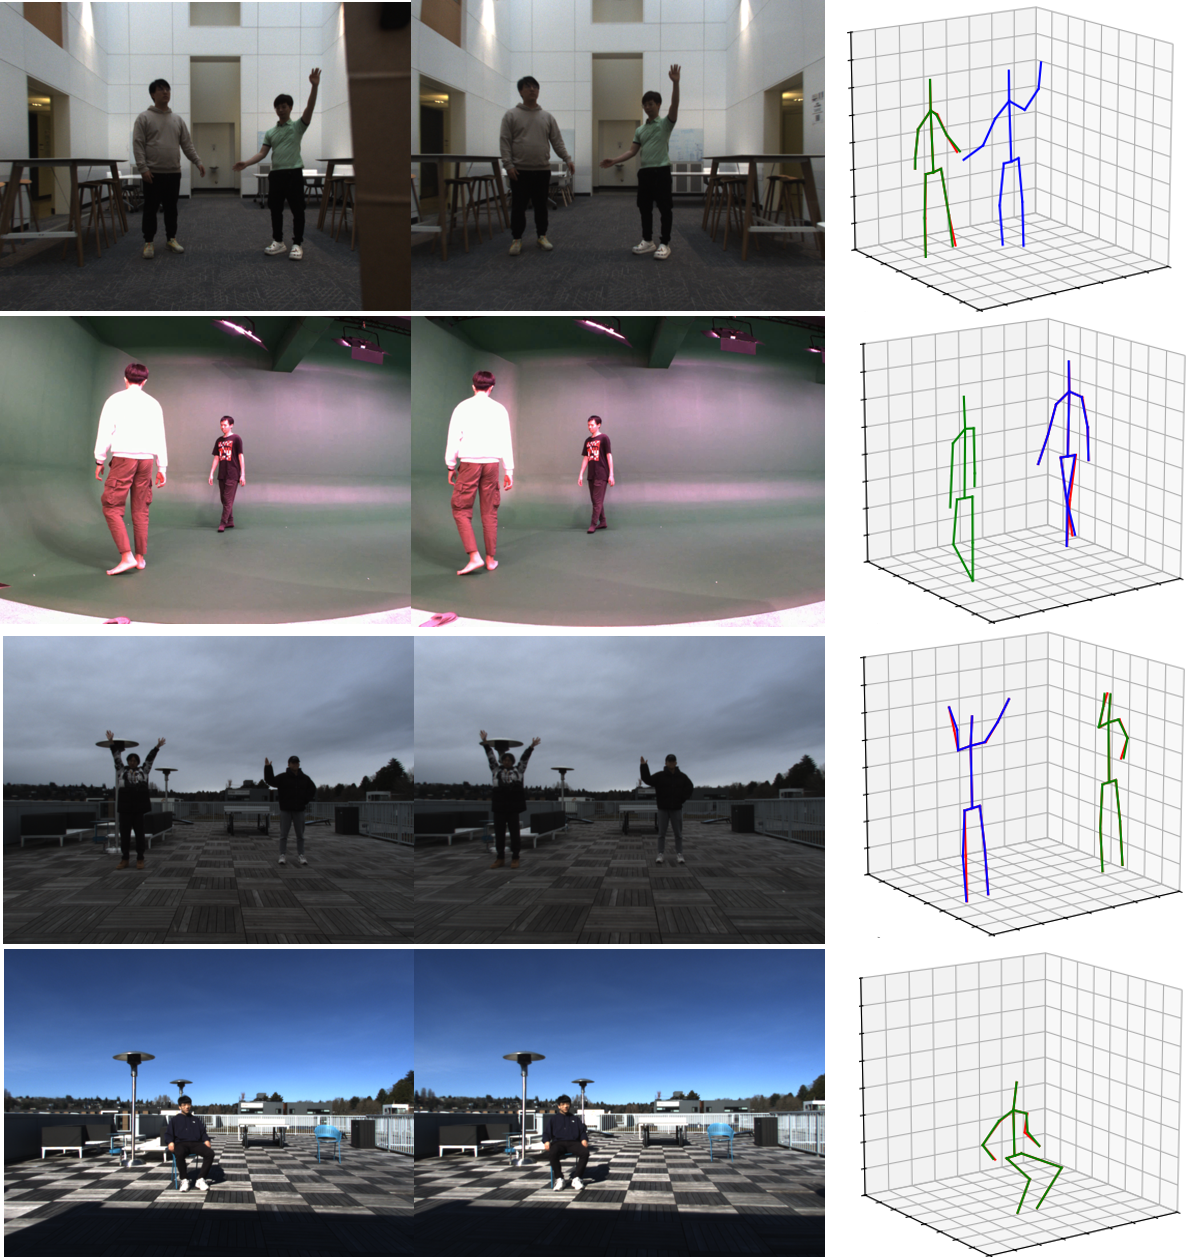
\includegraphics[width=0.85\textwidth]{images/rtpose_qualitative.png}
\caption{RT-Pose 数据集定性结果示例}
  \label{fig:rtpose_qualitative}
\end{figure}

\paragraph{多人场景效率与可扩展性}
为验证自底向上整图推理链路在多人场景下的效率优势，统计人数从 1 到 10 的端到端推理时延变化。图~\ref{fig:latency_vs_people}(a) 单独展示了自顶向下实例级管线 RTMW3D 的增长趋势：由于其包含“按人循环”的裁剪与回归步骤，时延随人数显著上升。图~\ref{fig:latency_vs_people}(b) 则聚焦于平稳区间内的对比，展示本文方法与 RTMO+MobileStereoNet（级联范式）在人数变化下近似恒定的时延表现。表~\ref{tab:latency_vs_people} 给出了关键人数点的数值对比：本文方法在 1 人与 10 人场景下时延分别为 116.0\,ms 与 117.3\,ms，仅增长约 1.1\%，体现出在拥挤多人场景下更稳定的端侧实时性。该稳定性与第~\ref{subsubsec:dwt}节可微加权三角化姿态求解器的设计一致：三维求解阶段仅对$M\times J$稀疏关节特征进行计算，不构建稠密深度/代价体，从而避免”无效像素”主导端侧时延。RTMO+MobileStereoNet 在不同人数下时延均为 189.2\,ms，保持恒定。这是因为其主要计算瓶颈在于对整幅图像逐像素执行稠密深度估计，该部分计算量只取决于输入分辨率而与场景人数无关；后续关节采样与三维恢复开销相对较小，不构成时延主导因素。尽管该级联范式同样具有人数无关的时延特性，但其端到端时延（189.2\,ms）仍显著高于本文方法（116.0--117.3\,ms），且在精度上（202.0\,mm vs 158.6\,mm）也存在较大差距，表明本文方法在精度与效率两方面均具备优势。

\begin{figure}[htbp]
  \centering
  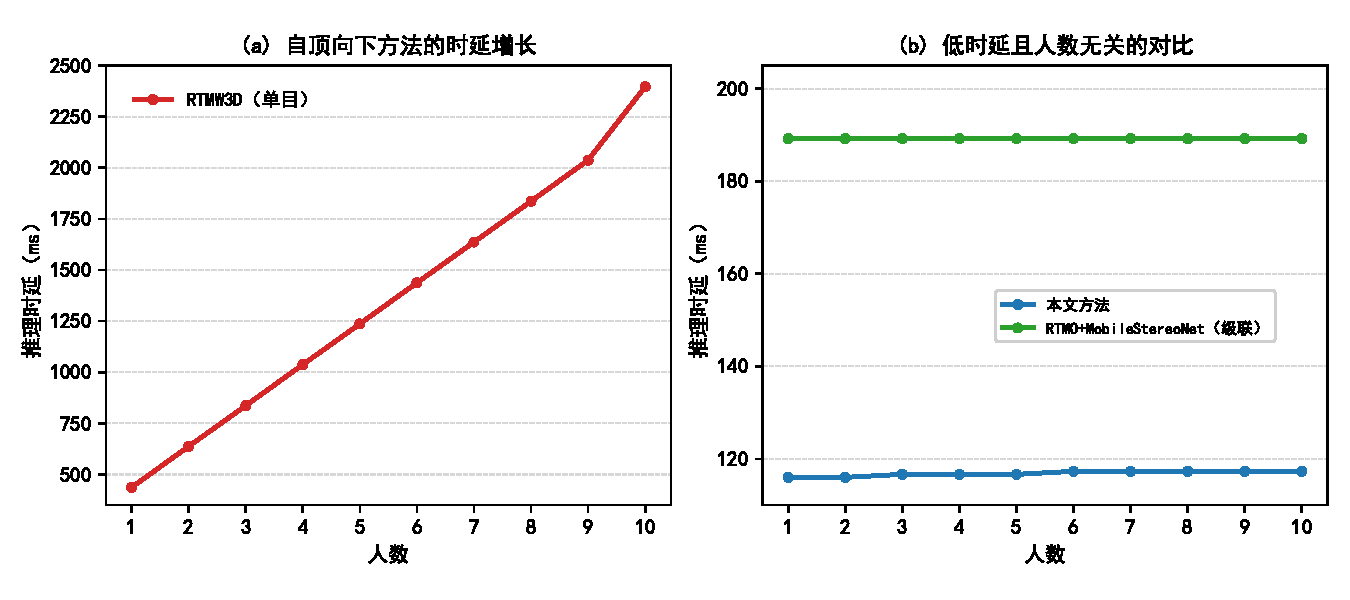
\includegraphics[width=0.92\textwidth]{images/latency_vs_people.pdf}
\caption{各方法推理时延随场景人数的变化对比}
  \label{fig:latency_vs_people}
\end{figure}

\begin{table}[htbp]
  \centering
  \small
\caption{不同人数下的端到端推理时延对比}
  \label{tab:latency_vs_people}
  \begin{tabular}{lccc}
    \toprule
    方法 & 1 人 & 5 人 & 10 人 \\
    \midrule
    本文方法（双目，自底向上） & 116.0 & 116.9 & 117.3 \\
    RTMW3D（单目，自顶向下） & 436.5 & 1236.8 & 2396.4 \\
    RTMO+MobileStereoNet（级联范式） & 189.2 & 189.2 & 189.2 \\
    \bottomrule
  \end{tabular}
\end{table}
\subsubsection{消融实验}
\noindent 以下所有消融实验均在 RT-Pose 测试集上进行，评价指标为左相机坐标系下的绝对 MPJPE（mm）。除特别说明外，各变体均在相同的数据划分、训练轮次与超参数设置下进行比较，其余训练与评测协议与主实验保持一致。当前各表报告的是固定随机种子下单次训练得到的点估计结果，尚未进行多种子重复训练，因此暂未写成“均值$\pm$标准差”。为便于把握整体贡献，消融部分先给出核心模块贡献汇总，再分别分析非对称骨干、EFEM、DWT 与跨分支一致性约束的作用。
\paragraph{模块贡献综合对比}
为综合呈现各核心模块对最终三维定位精度的贡献，表~\ref{tab:ablation_incremental} 以完整方法为基准，逐一将各模块替换为对照配置，并按精度退化幅度从大到小排列。各行数据来源于后续专项消融，此处仅作整体汇总。
\begin{table}[htbp]
  \centering
  \small
  \renewcommand{\arraystretch}{1.15}
\caption{核心模块贡献汇总}
  \label{tab:ablation_incremental}
  \begin{tabular}{lcc}
    \toprule
    配置描述 & Avg MPJPE(mm)$\downarrow$ & $\Delta$ vs.\ 完整方法 \\
    \midrule
    完整方法（非对称+EFEM+DWT+Align） & 158.6 & — \\
    EFEM $\rightarrow$ 无跨视图交互 & 374.5 & $+215.9$ \\
    DWT $\rightarrow$ 像素级三角化 & 277.7 & $+119.1$ \\
    EFEM $\rightarrow$ 拼接+$1\times1$卷积 & 224.8 & $+66.2$ \\
    非对称骨干 $\rightarrow$ 对称轻量骨干 & 182.0 & $+23.4$ \\
    Align $\rightarrow$ 移除（$\lambda_{\text{align}}=0$） & 175.3 & $+16.7$ \\
    \bottomrule
  \end{tabular}

  \vspace{2pt}
  \noindent\footnotesize 注：各行数据详见后文对应专项消融分析；$\Delta$ 均为正值，数值越大表明该模块贡献越显著。
\end{table}
\paragraph{非对称双目骨干网络（左重右轻）的贡献}
为验证“左重右轻”非对称双目骨干在精度与效率权衡上的有效性，本文对左右分支的骨干配置进行对比消融，结果如表~\ref{tab:ablation_asym_stereo} 所示。除骨干网络配置外，其余模块与训练/评测协议均保持一致。
\begin{table}[htbp]
  \centering
  \small
\caption{非对称双目骨干网络消融}
  \label{tab:ablation_asym_stereo}
  \begin{tabular}{lccc}
    \toprule
    双目骨干网络配置 & 参数量(M)$\downarrow$ & 计算量(G)$\downarrow$ & MPJPE(mm)$\downarrow$ \\
    \midrule
    左轻量 + 右轻量（对称轻量） & 7.6 & 9.2 & 182.0 \\
    左全量 + 右全量（对称全量） & 18.8 & 22.5 & 154.5 \\
    左全量 + 右轻量（非对称，本文） & 11.7 & 13.9 & 158.6 \\
    \bottomrule
  \end{tabular}
\end{table}

对称全量方案取得最低 MPJPE（154.5\,mm），但 FLOPs 较本文非对称方案高出约 62\%；对称轻量方案虽然更紧凑，却带来明显精度退化。这说明在本文面向端侧的双目场景中，右分支的主要作用是提供稳定的辅助几何观测，而非承担与左分支同等容量的语义表征任务，因此无需保持双侧对等配置。本文最终选择“左全量+右轻量”的非对称配置，在仅增加 4.1\,mm 误差的前提下显著压缩参数量与 FLOPs；其与实际端侧时延之间的对应关系将在第四章进一步分析。此外，第~\ref{sec:exp_setup}节采用的水平翻转并同步交换左/右视图的对称增强策略，有助于减弱非对称骨干对固定视角分工的依赖，使模型更关注稳定的双目几何对应关系，而非固化为依赖单一视角的偏置结构。

\paragraph{极线特征增强模块的贡献}
为验证极线特征增强模块的有效性，本文对不同跨视图特征交互方式进行对比，结果如表~\ref{tab:ablation_efem} 所示。
\begin{table}[htbp]
  \centering
  \small
\caption{跨视图特征交互方式对比}
  \label{tab:ablation_efem}
  \begin{tabular}{lc}
    \toprule
    特征增强模块 & MPJPE(mm)$\downarrow$ \\
    \midrule
    无跨视图交互 & 374.5 \\
    拼接+$1\times1$卷积 & 224.8 \\
    极线特征增强模块（本文） & 158.6 \\
    \bottomrule
  \end{tabular}
\end{table}

表~\ref{tab:ablation_efem} 表明，拼接+$1\times1$卷积虽能带来明显收益，但由于缺少显式几何约束，仍可能引入噪声匹配；EFEM 则在极线约束下将跨视图交互限制在一维视差窗口内，使匹配更具几何可解释性，从而进一步降低误差。“无跨视图交互”设置下虽然仍保留双目输入，但右视图轻量分支在遮挡与弱纹理场景下更易出现关键点多峰与定位抖动，导致视差误差在远距离小视差区域被放大；也就是说，此时非对称结构中的轻量右分支难以单独支撑稳定的跨视图几何约束。EFEM 通过沿极线引入低开销的跨视图一致性信息，可显著提升右分支观测的稳定性，从而释放双目几何在该数据集上的优势。

对视差搜索范围 $D_{\max}$ 的敏感性分析表明，$D_{\max}=96$ 在覆盖有效匹配与抑制噪声相关之间取得最佳平衡（$D_{\max}=32/64/96/128$ 对应 MPJPE 分别为 171.5/162.0/158.6/160.2\,mm），范围过小时有效视差不足，过大时背景候选稀释匹配响应，精度均有回退，因此本文取 $D_{\max}=96$ 作为默认设置。

\paragraph{可微加权三角化姿态求解器的贡献}
为分析三维恢复策略对最终精度的影响，将本文的可微加权三角化姿态求解器与两种简化方案进行对比，结果如表~\ref{tab:ablation_solver} 所示。其中，“直接深度回归”指在二维关节观测基础上直接预测关节深度而不显式引入相机投影约束的回归式三维恢复基线。像素级关键点匹配+三角化受限于二维定位精度，直接深度回归则缺少显式投影约束；本文求解器通过 softargmax 提供可微二维观测，并利用置信度权重抑制不可靠视角约束，因此可获得更稳健的三维解。
\begin{table}[htbp]
  \centering
  \small
\caption{三维恢复策略对比}
  \label{tab:ablation_solver}
  \begin{tabular}{lc}
    \toprule
    三维恢复策略 & MPJPE(mm)$\downarrow$ \\
    \midrule
    2D 关键点匹配（像素级）+三角化 & 277.7 \\
    直接深度回归 & 225.1 \\
    可微加权三角化姿态求解器（本文） & 158.6 \\
    \bottomrule
  \end{tabular}
\end{table}

进一步的组件消融表明，softargmax 与置信度加权均能带来稳定收益：MPJPE 由不可导且无加权时的 182.5\,mm 依次降至 168.0\,mm 和 158.6\,mm。在当前实现中，式\eqref{eq:pdrm_softmax2d} 的 softargmax 温度固定为$\tau=1$，不引入可学习温度参数。两者共同构成了 DWT 性能提升的主要来源。

\paragraph{跨分支表征一致性约束的贡献}
针对“左重右轻”非对称结构可能带来的表征差异，本文在训练阶段引入跨分支表征一致性约束，以提升轻量分支的几何敏感性与稳定性；该约束仅作用于训练阶段，推理时对应分支与损失项均被移除，不引入额外计算开销。表~\ref{tab:ablation_align} 对比了不同一致性约束形式的效果。结果显示，引入特征对齐正则均可降低误差，其中“$1\times1$对齐卷积+MSE”效果最好，说明该形式更适合处理跨分支连续特征对齐问题；KL 散度对齐在本文中仅作为对比项使用，其实现细节不再展开。
\begin{table}[htbp]
  \centering
  \small
\caption{跨分支一致性约束形式对比}
  \label{tab:ablation_align}
  \begin{tabular}{lcc}
    \toprule
    一致性约束形式 & MPJPE(mm)$\downarrow$ & 提升(\%) \\
    \midrule
    不使用一致性约束 & 175.3 & -- \\
    KL 散度对齐 & 168.9 & 3.7\% \\
    余弦相似度对齐 & 165.2 & 5.8\% \\
    $1\times1$对齐卷积+MSE（本文） & 158.6 & 9.5\% \\
    \bottomrule
  \end{tabular}
\end{table}

对约束权重 $\lambda_{\text{align}}$ 的敏感性分析表明，过小时引导不足，过大时会干扰主任务优化；在测试的 $0.01$--$1.0$ 范围内，$\lambda_{\text{align}}=0.1$ 取得最佳结果（158.6\,mm），因此被设为默认值。

\subsection{本章小结}

本章围绕端侧多人三维人体姿态估计任务，针对现有双目方法在稠密级联开销与左右对称冗余两方面的瓶颈，提出了一种轻量化非对称双目学习框架。

方法上，本文并未沿用“稠密深度估计+关节回代”的重型级联思路，而是围绕关节级几何任务重新组织双目信息流：一方面通过“左重右轻”的非对称骨干与跨分支一致性约束压缩冗余计算并保持轻量分支表征能力；另一方面通过 EFEM 建立受极线约束的低开销跨视图匹配，并结合可微加权三角化求解器，将二维热力图观测、视图置信度与显式投影约束统一到端到端三维恢复链路之中。

实验结果表明，本文方法在 RT-Pose 上达到 $158.6$\,mm 的平均绝对 MPJPE，相较最优级联范式降低 $43.4$\,mm；同时，在 Xiaomi 14 上从 1 人到 10 人场景的端到端时延仅增加 $1.3$\,ms，体现出自底向上整图推理链路在多人场景下的稳定可扩展性。

本文第三章的主要实验仍以 RT-Pose 为核心验证基准，虽然进一步补充了 RT-Pose$\rightarrow$MADS 的零样本泛化测试，但对标定扰动、外参误差与更广泛双目采集协议差异的影响尚未进行系统量化，这些问题仍有待在后续工作中进一步展开。

第三章的关键贡献在于证明：在不依赖稠密深度中间表示的前提下，双目三维人体姿态估计仍可通过结构轻量化、几何约束驱动的跨视图交互与可微三维求解实现精度与效率的统一。这也为下一章进一步开展硬件感知部署与量化压缩提供了方法基础。
\newpage
\section{硬件感知部署与量化压缩}

本章面向第三章所提轻量化双目三维人体姿态估计框架的端侧落地问题，围绕 Snapdragon 8 Gen3 CPU 平台上的硬件感知部署与量化压缩展开研究。研究重点不在于比较不同硬件后端，而在于针对既定端侧 CPU 执行环境，建立从性能瓶颈定位到混合精度设计与实证验证的完整方法链。本文首先通过实测延迟拆解与 Roofline 分析定位性能瓶颈，随后结合量化敏感性分析设计分层混合精度方案，并通过后训练量化（PTQ）完成部署，最终以对比实验与消融实验评估量化后的精度--效率综合表现。

\subsection{研究背景}
多人三维人体姿态估计正从离线精度导向的算法研究转向端侧实时应用。在移动机器人、智能安防与沉浸式交互等场景中，系统不仅需要满足严格时延约束，还需尽量避免原始图像上传云端带来的隐私风险与网络依赖。因此，如何在移动端或嵌入式设备上稳定运行三维姿态估计模型，已成为影响其实用化的重要问题。

从任务建模角度看，双目方案之所以值得关注，在于其在几何约束强度与工程落地成本之间提供了更均衡的折中。单目三维姿态估计虽然硬件成本最低，但在复杂遮挡、尺度变化与大幅动作条件下容易受到深度歧义与绝对尺度不确定性的限制；多目系统虽然能够提供更强的空间约束，却往往伴随更高的硬件成本、更复杂的同步标定流程以及更苛刻的安装条件，难以作为移动端的通用配置。双目系统能够借助视差与三角测量显式引入深度线索，在硬件复杂度、部署成本与三维恢复稳定性之间取得更可行的工程平衡，因此更适合作为端侧三维人体姿态恢复的传感器基础。

但双目几何优势并不意味着部署过程天然轻量。对于本文的整图双目推理模型而言，跨视图匹配、特征交互与几何恢复在带来深度信息的同时，也引入了额外的卷积算力开销、权重与激活访存压力，以及对数值误差更敏感的 softmax 归一化和几何求解链路。移动端 CPU 与边缘设备通常同时受到算力、内存带宽、缓存容量与功耗预算的约束，模型能否落地不仅取决于参数规模，还取决于权重访存模式、算子调度方式以及中间激活的存取开销。现有工作通常将结构裁剪、算子优化与量化部署协同设计\cite{jacob2018quantization,banner2019post,nagel2019data,xiao2023smoothquant}；这也说明，端侧量化并非“全模型一刀切”即可达到最优效果，精度风险往往集中在激活分布不稳定层、归一化与匹配相关环节，以及直接参与几何恢复的求解环节。基于上述背景，本章首先分析端侧瓶颈与量化风险，再据此设计兼顾精度、时延与模型体积的混合精度部署方案。

\subsection{问题分析}

本节围绕“哪些模块最值得量化、哪些模块不能轻易量化”这一核心问题展开。具体分为三步：首先通过实测延迟拆解识别优化重点，其次借助 Roofline 模型分析热点形成瓶颈的原因，最后通过量化敏感性分析确定哪些层适合量化、哪些层必须保护。

\subsubsection{端侧推理瓶颈的实测分析}

4.2.1 首先探究端侧推理时间主要分布在哪些模块。为定位第三章所提框架在端侧的计算热点，本节以 Xiaomi 14 为目标平台，在 MNN、FP16、ARMv8.2、4 线程、输入 $640\times480$、batch=1、单人场景下对各模块逐一计时。

各模块实测延迟如表~\ref{tab:module_latency} 所示。

\begin{table}[htbp]
  \centering
  \small
  \caption{各模块实测延迟}
  \label{tab:module_latency}
  \begin{tabular}{lccl}
    \toprule
    模块 & 延迟 (ms) & 占比 (\%) & 主要算子类型 \\
    \midrule
    左分支骨干 & 76.7 & 66.1 & Conv, BN, SiLU, CSP \\
    右分支骨干 & 19.4 & 16.7 & Conv, BN, SiLU, CSP \\
    极线特征增强模块            & 10.0 &  8.6 & 1$\times$1 Conv, 矩阵乘，Softmax \\
    热力图头与置信度头                   &  7.0 &  6.0 & 1$\times$1 Conv \\
    可微加权三角化求解器         &  1.1 &  0.9 & Softmax, 矩阵乘, 特征值分解 \\
    \midrule
    端到端合计                           & 116.0 & 100.0 & -- \\
    \bottomrule
  \end{tabular}
\end{table}

\begin{figure}[htbp]
  \centering
  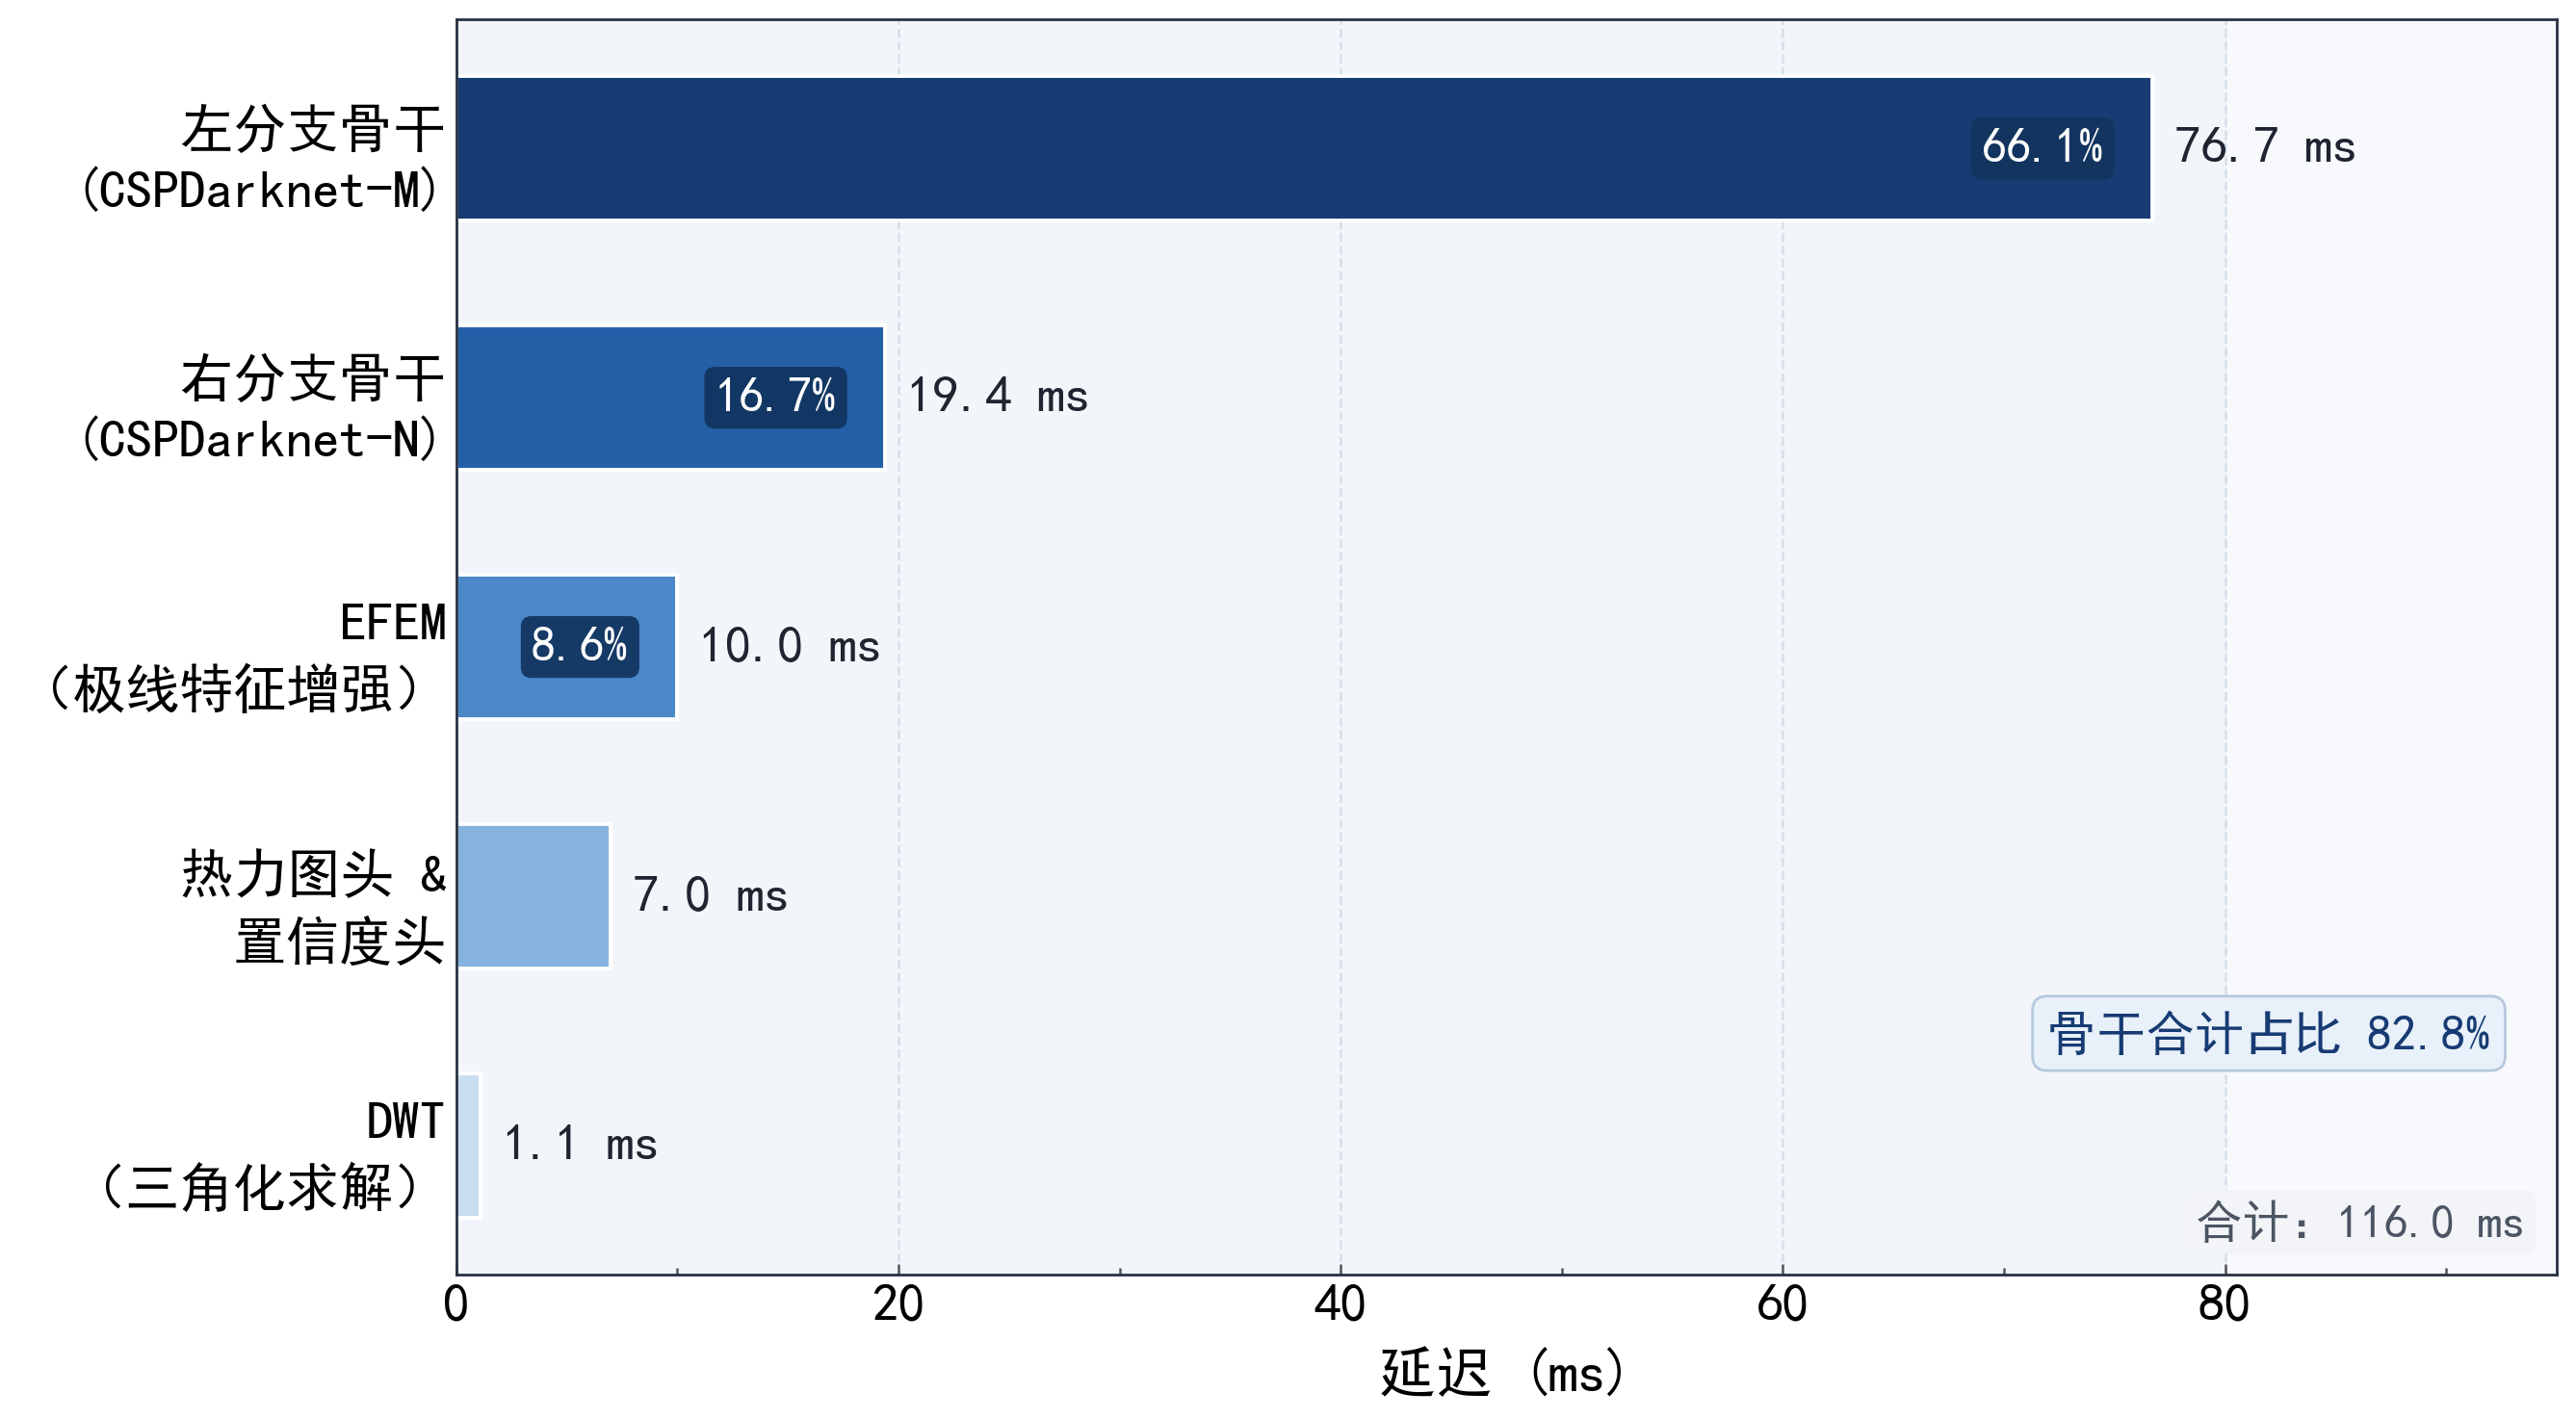
\includegraphics[width=0.88\textwidth]{images/ModuleDelayRatioFanChart}
  \caption{各模块端到端延迟占比}
  \label{fig:module_delay_pie}
\end{figure}

由表~\ref{tab:module_latency} 与图~\ref{fig:module_delay_pie} 可知，骨干网络是延迟主体；图~\ref{fig:cspdarknet_stage_pie} 进一步给出骨干内部各阶段的延迟分布。

\begin{figure}[htbp]
  \centering
  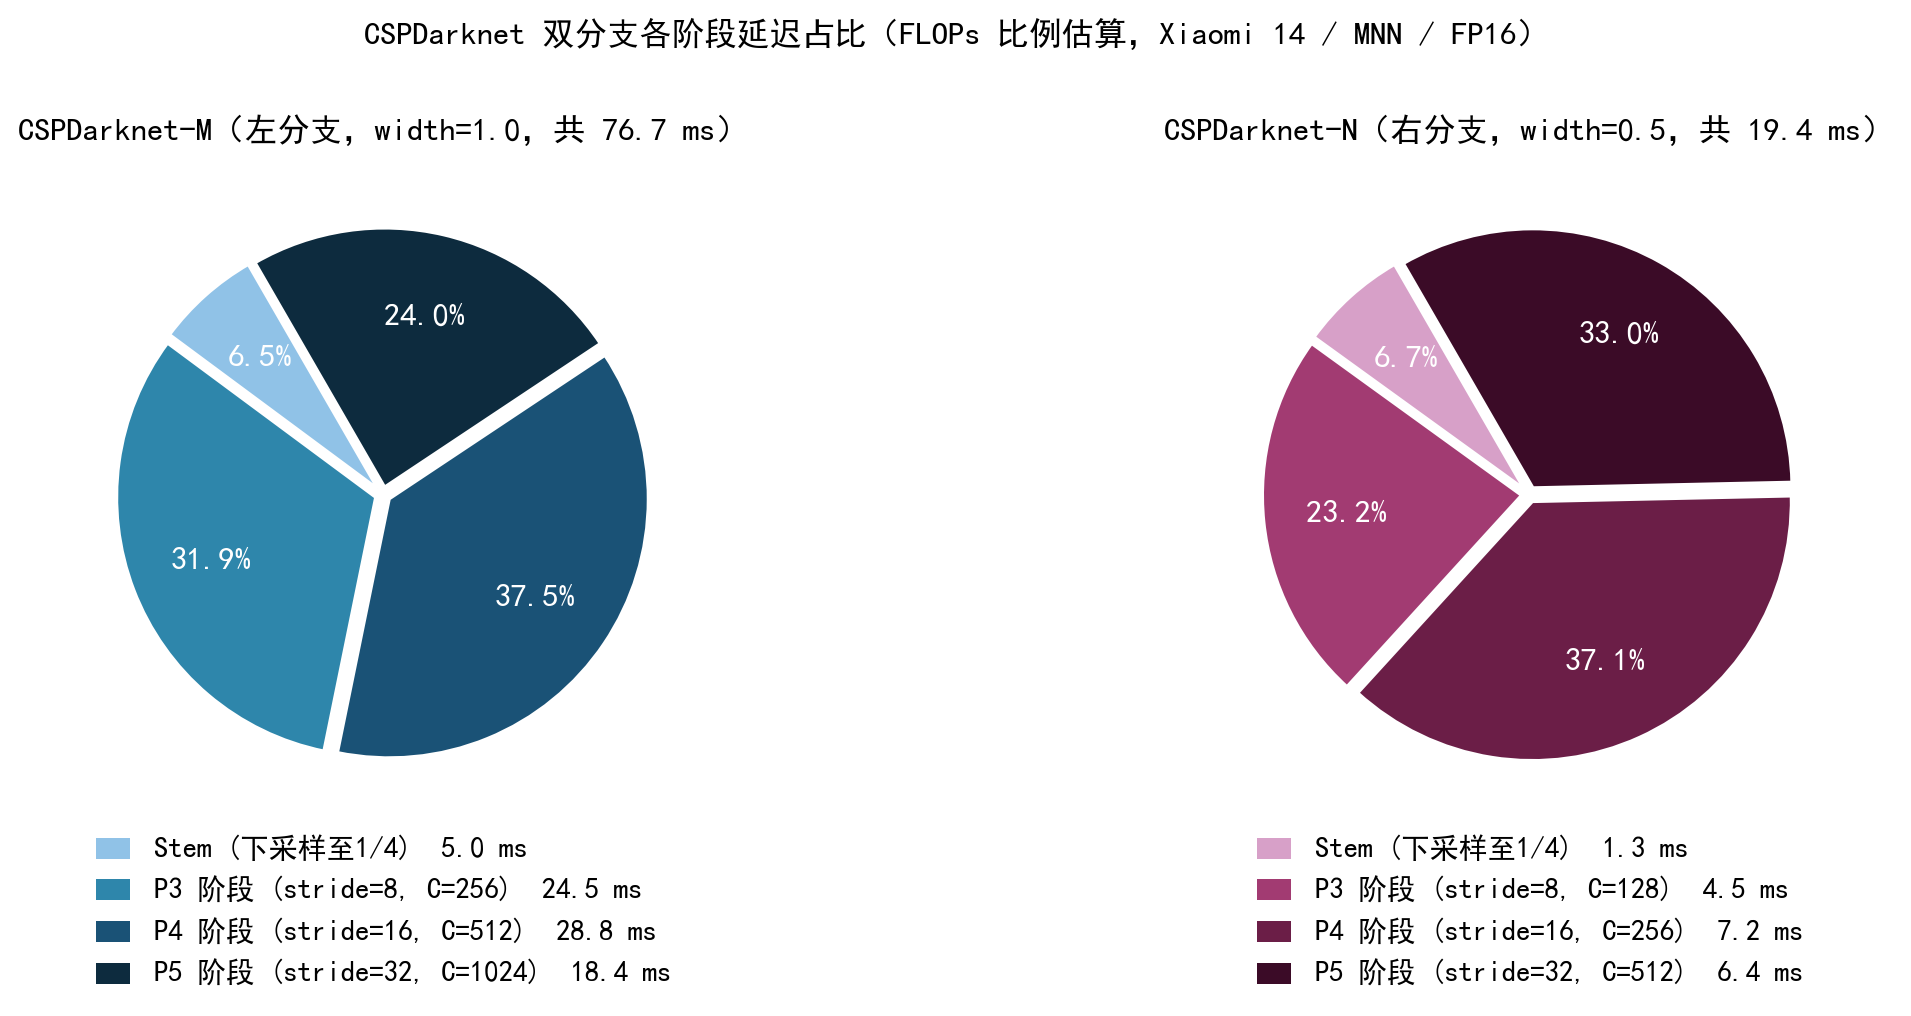
\includegraphics[width=0.96\textwidth]{images/CSPDarknetStageLatencyPie}
  \caption{CSPDarknet 各阶段延迟占比}
  \label{fig:cspdarknet_stage_pie}
\end{figure}

从结构上看，CSPDarknet 对 INT8 量化具有较好的适应性：骨干中的 Conv-BN 可在图优化阶段融合，SiLU 与 BN 融合后的权重分布也更利于 per-channel 对称量化；同时，左分支与右分支 76.7\,ms 和 19.4\,ms 的延迟比与理论计算量比基本一致，说明骨干延迟主要由卷积算术负载决定，INT8 dotprod 加速可直接转化为时延收益。图~\ref{fig:cspdarknet_stage_pie} 进一步表明，P3/P4 阶段合计约占各分支延迟 70\%，是骨干内部最值得优先量化的主加速区；相比之下，Stem 占比较低，P5 受分辨率下降影响，其绝对开销也低于 P4。

由表~\ref{tab:module_latency}、图~\ref{fig:module_delay_pie} 与图~\ref{fig:cspdarknet_stage_pie} 可得到以下结论：

（1）骨干网络是端侧延迟的绝对主体，左右两分支合计占据端到端总延迟的大部分，其中左分支由于通道宽度更大而成为首要优化热点。

（2）骨干内部又以 P3/P4 为最值得优先量化的主加速区，INT8 收益预计主要来自这一部分主体卷积。

（3）EFEM 虽然占比次于骨干，但由于存在不规则访存，其收益模式不能仅凭 FLOPs 判断，需要在 4.2.2 节进一步辨别其究竟受算力还是带宽约束。

（4）可微加权三角化求解器延迟占比不足 1\%，在性能侧不构成量化重点。

\subsubsection{Roofline 分析：访存密集型与计算密集型模块辨别}

在确认“骨干是主热点、EFEM 是次级热点”之后，本节进一步分析这些热点形成瓶颈的原因，以及量化收益主要来自哪里。为此，引入 Roofline 模型以算术强度（Arithmetic Intensity, AI）刻画算子“算得多还是搬得多”，其中
$\mathrm{AI}=\text{FLOPs}/\text{bytes}$（FLOP/byte）。在给定硬件上，理论可达性能满足
\[
  P \le \min\!\bigl(P_{\text{peak}},\, B_{\text{eff}}\cdot \mathrm{AI}\bigr),
\]
其中 $P_{\text{peak}}$ 为计算峰值、$B_{\text{eff}}$ 为有效带宽。该模型用于判断各模块属于“计算密集”还是“访存密集”。


之所以采用 $B_{\text{eff}}$ 而非 $B_{\text{peak}}$，是因为推理阶段存在明显的 LLC 容量瓶颈：FP16 基线权重约 23.4\,MB，显著超过 LLC（8\,MB），骨干权重难以整体驻留片上，前向过程中需要按层从 LPDDR5X 流水加载。表~\ref{tab:memory_hierarchy} 给出存储层次参数。

实验平台为 Xiaomi\,14（Snapdragon 8 Gen3，大核集群 1×Cortex-X4@3.3\,GHz + 3×Cortex-A720@3.15\,GHz）。在 NEON FP16 下取 4 线程理论峰值算力
$P_{\text{peak}}\approx100\,\text{GFLOPS}$；LPDDR5X 双通道理论带宽
$B_{\text{peak}}\approx68\,\text{GB/s}$。推理阶段由于缓存缺失与控制器利用率等因素，采用更符合实际的有效带宽
$B_{\text{eff}}\approx40\,\text{GB/s}$。由此屋脊点为
\[
  \mathrm{AI}_{\text{ridge}}=\frac{P_{\text{peak}}}{B_{\text{eff}}}\approx2.5\,\text{FLOP/byte},
\]
因此 $\mathrm{AI}<2.5$ 的算子主要受带宽约束，$\mathrm{AI}>2.5$ 的算子主要受算力约束。

\begin{table}[htbp]
  \centering
  \small
\caption{骁龙 8 Gen3 存储层次参数}
  \label{tab:memory_hierarchy}
  \begin{tabular}{llll}
    \toprule
    层次 & 容量 & 典型带宽（估算） & 推理阶段角色 \\
    \midrule
    L2 Cache     & 512\,KB–2\,MB & $\sim$200\,GB/s & 热点小算子局部复用 \\
    LLC（共享 L3） & 8\,MB         & $\sim$80\,GB/s  & 权重驻留能力瓶颈 \\
    LPDDR5X      & 12\,GB        & 68\,GB/s（理论） & 权重按层流水加载来源 \\
    UFS 4.0      & 片上存储       & $\sim$4\,GB/s   & 模型加载阶段（一次性） \\
    \bottomrule
  \end{tabular}
\end{table}

在上述硬件参数下，进一步估算各模块在 FP16、batch=1 条件下的 AI。对于 $3\times3$ 卷积（输入通道 $C_{\text{in}}$、输出通道 $C_{\text{out}}$、分辨率 $H\!\times\! W$），有
\[
  \mathrm{AI}_{3\times3}
  = \frac{2\,C_{\text{in}}\cdot 9\cdot C_{\text{out}}\cdot HW}
         {2\bigl(9\,C_{\text{in}}\,C_{\text{out}}
                 + C_{\text{in}}\,HW
                 + C_{\text{out}}\,HW\bigr)}
\]
骨干三尺度 $3\!\times\!3$ 卷积的 $\mathrm{AI}\approx280$--$923$\,FLOP/byte，远高于 $\mathrm{AI}_{\text{ridge}}$，属于计算密集型；EFEM 中 $1\!\times\!1$ 投影卷积与热力图头 $1\!\times\!1$ 卷积虽位于屋脊点右侧，但更靠近屋脊点，更容易受到带宽与调度开销影响；EFEM 的 gather/correlation（视差维度 $D\!=\!24$ 的逐位移采样与点积）$\mathrm{AI}\approx0.04$\,FLOP/byte，为极端访存密集型。表~\ref{tab:roofline_summary} 汇总各模块的 AI 与瓶颈类型。

\begin{table}[htbp]
  \centering
  \small
\caption{各模块算术强度与瓶颈类型}
  \label{tab:roofline_summary}
  \begin{tabular}{llcc}
    \toprule
    模块 & 主要算子 & AI (FLOP/byte) & 瓶颈类型 \\
    \midrule
    左/右骨干（stride=8，$C=256$）  & $3\times3$ Conv & 923 & 计算密集 \\
    左/右骨干（stride=16，$C=512$） & $3\times3$ Conv & 784 & 计算密集 \\
    左骨干（stride=32，$C=1024$）   & $3\times3$ Conv & 280 & 计算密集 \\
    EFEM 投影（$1\times1$ Conv）    & $1\times1$ Conv & 11.3 & 屋脊点附近 \\
    EFEM gather/correlation         & 逐视差切片点积  & 0.04 & 极端访存密集 \\
    热力图/置信度头                  & $1\times1$ Conv & 15.7 & 屋脊点附近 \\
    DWT 三角化                       & 矩阵乘/特征值  & ---  & 计算量可忽略 \\
    \bottomrule
  \end{tabular}
\end{table}


图~\ref{fig:roofline} 给出理论可达点与实测工作点的对比。骨干卷积位于计算密集区，EFEM gather 位于极端访存密集区，EFEM 投影与预测头则靠近屋脊点，说明它们更容易同时受到带宽与调度开销影响。

需要说明的是，图中的“实测工作点”并非逐算子硬件性能计数器的直接采样值，而是由模块级时延统计结合算术强度估算得到，用于反映不同模块在目标平台上的相对瓶颈位置，而非作为绝对硬件计数结果。

\begin{figure}[htbp]
  \centering
  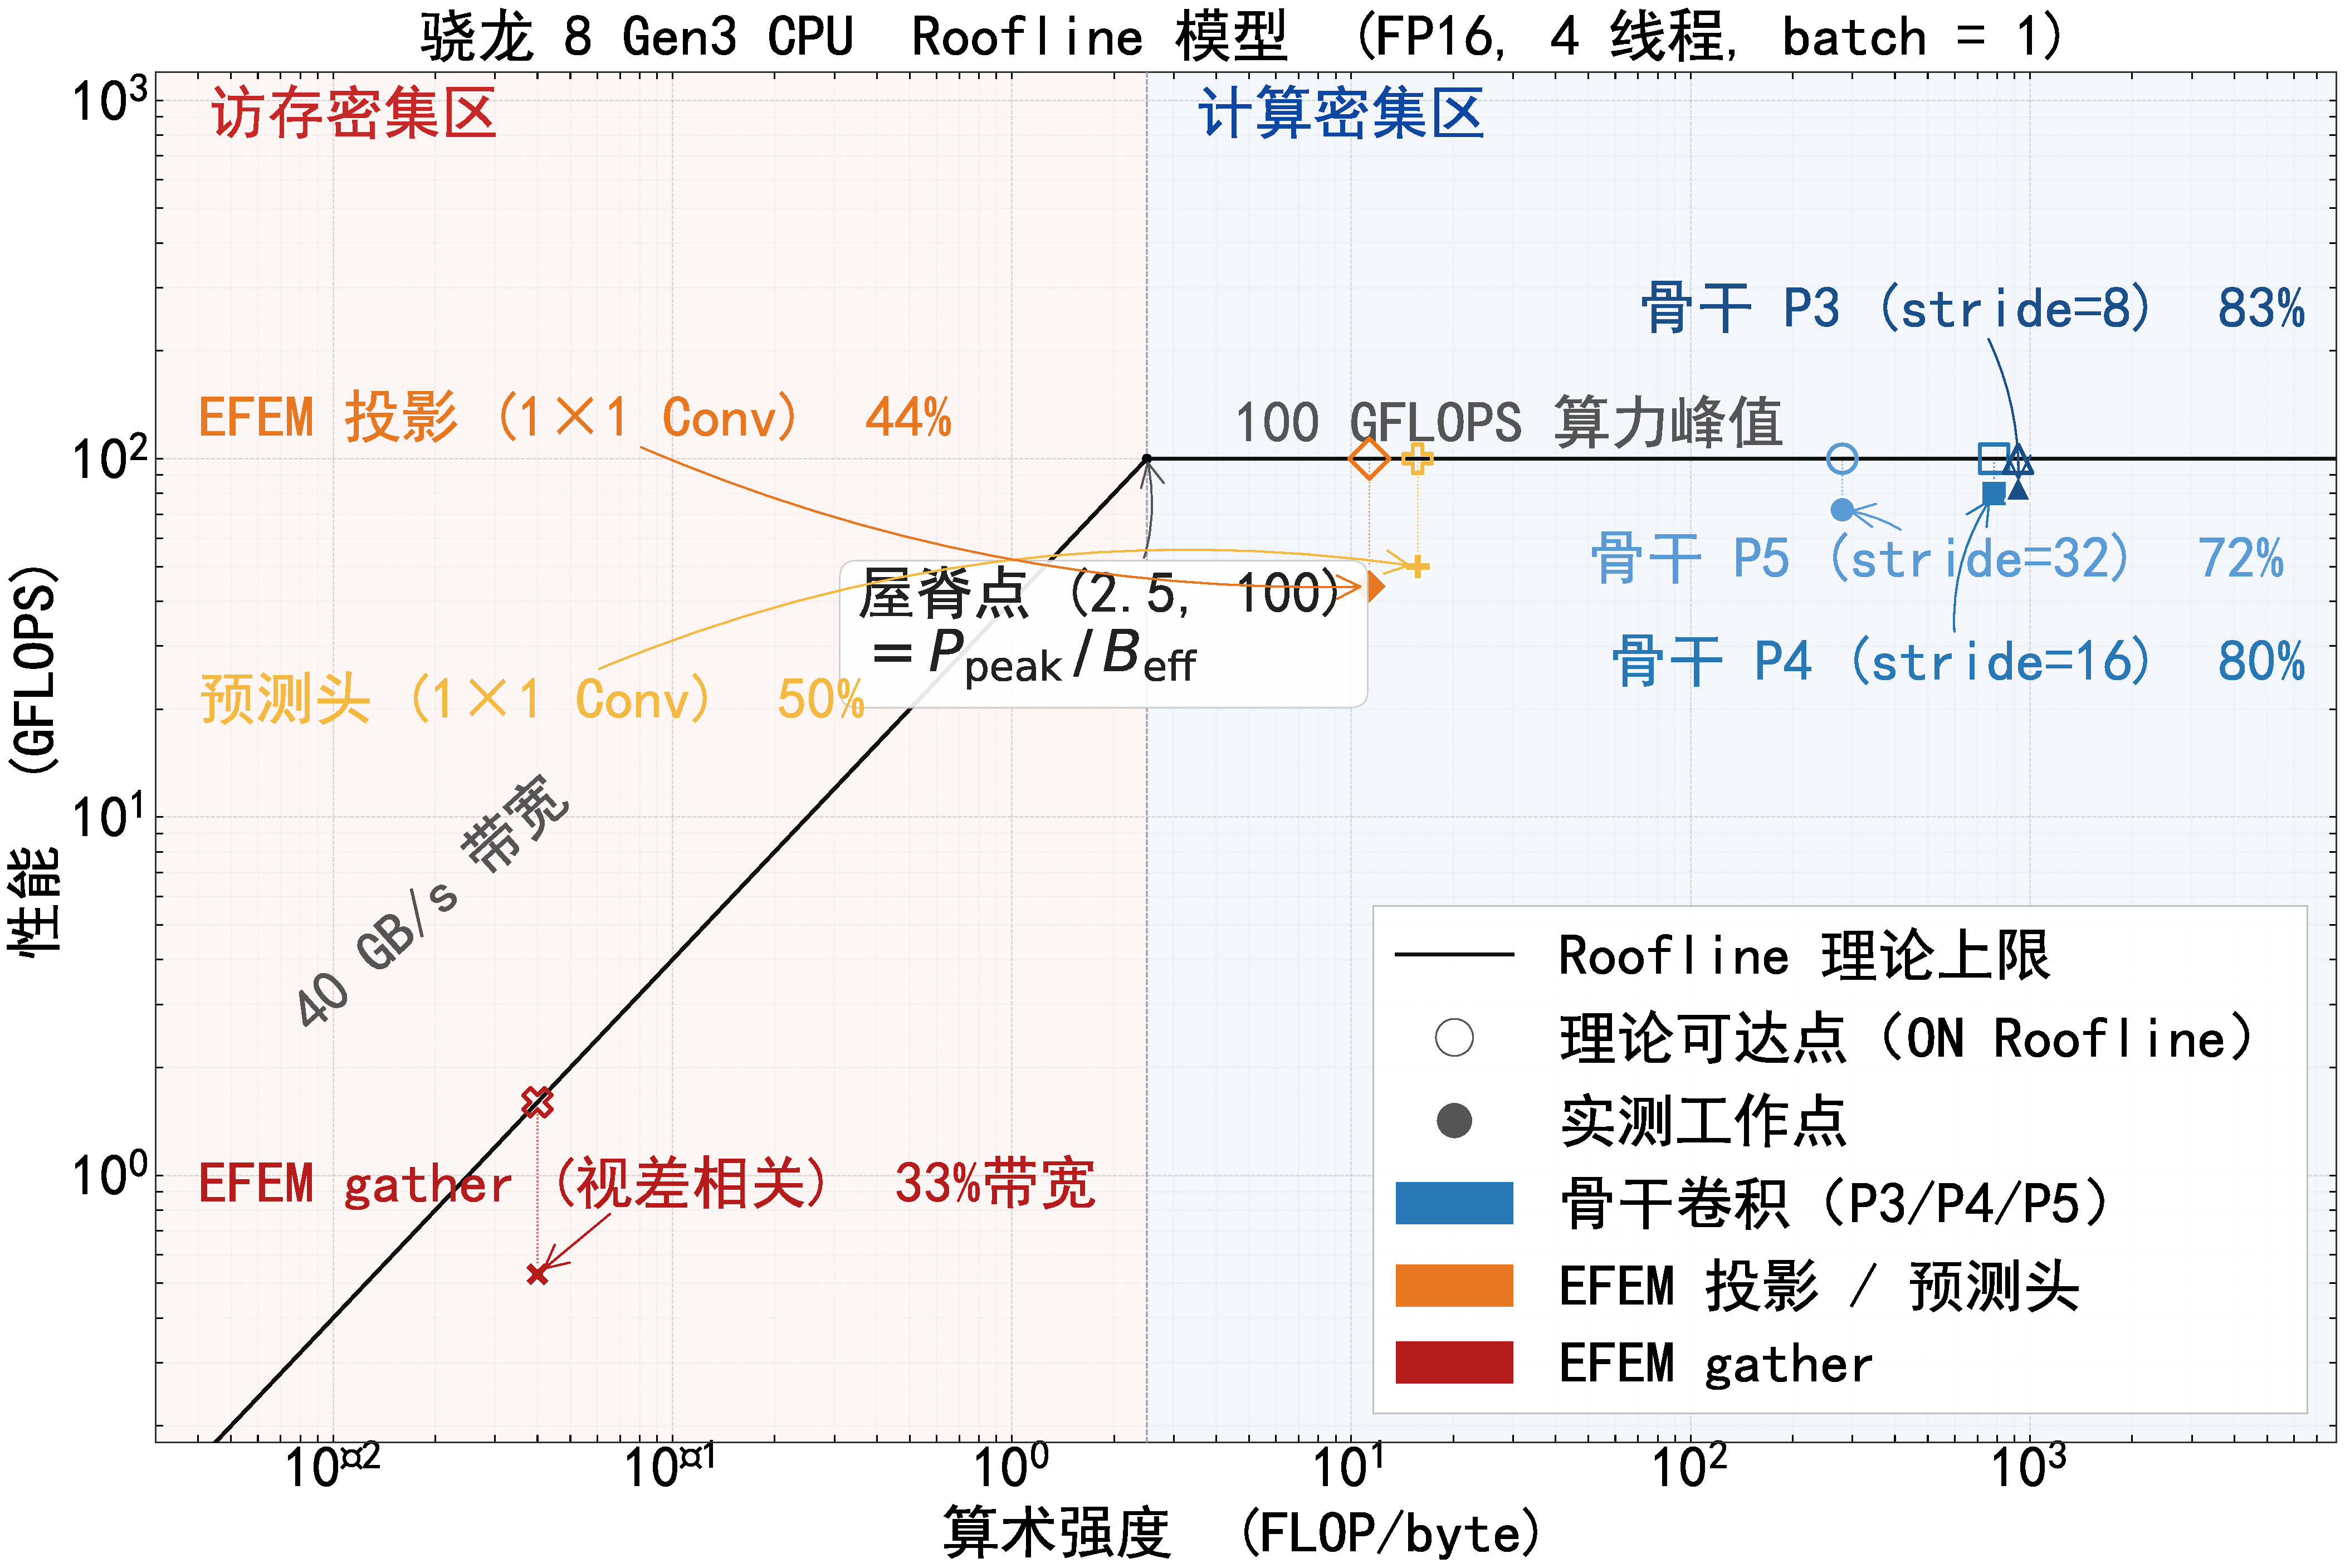
\includegraphics[width=0.82\textwidth]{images/roofline.pdf}
  \caption{各模块 Roofline 分析}
  \label{fig:roofline}
\end{figure}

综合图~\ref{fig:roofline} 与表~\ref{tab:roofline_summary} 可得到以下结论：

（1）骨干卷积的瓶颈主要位于算力侧，INT8 可借助 ARMv8.2 dotprod 将 4 线程吞吐提升至约 FP16 的 $2\times$（约 200\,GOPS），从而直接缩短主体卷积耗时。

（2）EFEM 投影、头部卷积及 gather 更接近或落在带宽受限区域，INT8 权重的主要收益来自减少 DRAM 读入字节数（2\,B/param $\rightarrow$ 1\,B/param）并提升缓存命中率。

（3）后续量化方案应将“骨干卷积作为主要加速来源、将 EFEM gather 等访存密集算子视作收益受限对象”作为基本原则。

（4）在该瓶颈结构下，端到端收益预期约为 1.5--1.7$\times$ 延迟加速，并伴随约 $2\times$ 的模型压缩（具体取决于分层混合精度的权重占比）。

\subsubsection{量化敏感性分析}

4.2.3 最后重点考察哪些热点可以量化、哪些关键环节必须保护。本节以第三章 FP16 模型为基线，在 RT-Pose 验证集上采用逐组替换方式评估各模块的 INT8 敏感性：每次仅将某一模块的权重或激活替换为 INT8，其余模块保持 FP16，并记录相对基线的 $\Delta\text{MPJPE}$。

\begin{table}[htbp]
  \centering
  \small
\caption{各模块 INT8 量化敏感性分析}
  \label{tab:quant_sensitivity}
  \begin{tabular}{@{}p{0.31\textwidth}p{0.10\textwidth}p{0.16\textwidth}p{0.10\textwidth}p{0.19\textwidth}@{}}
    \toprule
    量化目标 & 量化类型 & $\Delta$MPJPE (mm)$\uparrow$ & 敏感等级 & 推荐处置 \\
    \midrule
    骨干 Conv+BN 权重（左分支）            & 权重 & $+1.8$ & 低   & INT8 per-channel \\
    骨干 Conv+BN 权重（右分支）            & 权重 & $+1.4$ & 低   & INT8 per-channel \\
    EFEM 投影权重（$\varphi_q/\varphi_k/\varphi_v$）& 权重 & $+2.1$ & 低   & INT8 per-channel \\
    EFEM 注意力分数（激活）                & 激活 & $+6.8$ & 高   & 保留 FP32 \\
    热力图头输出（激活）                   & 激活 & $+3.2$ & 中   & 保留 FP32 \\
    置信度头输出（激活）                   & 激活 & $+4.1$ & 中   & 保留 FP32 \\
    DWT 输入/输出（激活）                  & 激活 & $+7.3$ & 极高 & 保留 FP32 \\
    \bottomrule
  \end{tabular}
\end{table}

这些高敏感模块都直接处在匹配分布、峰值判别或几何求解链路上，量化误差更容易被放大。综合表~\ref{tab:quant_sensitivity} 与 MNN CPU 推理对混合精度的实现方式（量化豁免层以 FP32 执行），可得到以下结论：

（1）骨干与 EFEM 投影的权重量化整体低敏感（$\Delta\text{MPJPE}<2.5$\,mm），可作为后续 INT8 量化的主要覆盖对象。

（2）EFEM 注意力分数与 DWT 求解相关激活对量化高度敏感（$\Delta\text{MPJPE}\approx6.8$--$7.3$\,mm），应作为精度保护层。

（3）热力图与置信度头输出激活呈中等敏感（$+3$--$4$\,mm），为避免峰值判别退化，同样建议保护。


\subsection{混合精度量化方案设计}

本节将前述瓶颈分析与敏感性筛查统一到同一设计框架下。本文采用“三步式”决策路径：先定位性能瓶颈，再识别高风险层，最后据此设计分层混合精度与 PTQ 校准流程；目标是在保持几何推理稳定性的前提下，最大化主体卷积层的 INT8 覆盖率。

\subsubsection{分层精度分配方案}

4.3.1 的目标是把 4.2 的分析结果落到可执行的精度分配上。依据“性能贡献 $\times$ 数值风险”的联合标准，骨干与 EFEM 的主体卷积层作为 INT8 的主要覆盖对象；EFEM 注意力分数、热力图/置信度输出以及 DWT 求解器则统一保留为 FP32 保护路径。保护层采用 FP32 的依据既来自敏感性分析，也与当前 MNN CPU 混合精度执行路径对量化豁免层的实现方式一致。主体卷积采用 INT8 权重与激活联合量化，权重量化选用 per-channel 对称方案；EFEM 的投影与融合卷积参与 INT8 校准，但 gather/correlation 不作为独立 INT8 加速对象处理。具体分层方案如表~\ref{tab:precision_allocation} 所示。

\begin{table}[htbp]
  \centering
  \small
  \caption{本文分层混合精度量化方案}
  \label{tab:precision_allocation}
  \begin{tabular}{@{}p{0.27\textwidth}p{0.12\textwidth}p{0.17\textwidth}p{0.30\textwidth}@{}}
    \toprule
    模块 & 操作对象 & 分配精度 & 设计依据 \\
    \midrule
    左骨干（全部 Conv+BN）                  & 权重+激活 & INT8 & 低敏感；计算/访存密集 \\
    右骨干（全部 Conv+BN）                  & 权重+激活 & INT8 & 低敏感；计算/访存密集 \\
    EFEM 投影（$\varphi_q/\varphi_k/\varphi_v$）& 权重+激活 & INT8 & 低敏感；访存密集 \\
    EFEM gather/correlation               & 激活 & FP32（不量化） & 极端访存密集；非规则访存，不作为独立 INT8 主收益来源 \\
    EFEM 注意力分数（scores）               & 激活 & FP32（不量化）   & 高敏感；视差匹配精度 \\
    EFEM 聚合与融合（$\psi$）               & 权重+激活 & INT8 & 低敏感 \\
    热力图头（左/右）                       & 权重+激活 & FP32（不量化）& 中敏感；坐标回归精度 \\
    置信度头（左/右）                       & 权重+激活 & FP32（不量化）& 中敏感；权重自适应精度 \\
    DWT 三角化求解器                        & 全部 & FP32（不量化）   & 极高敏感；数值稳定性 \\
    \bottomrule
  \end{tabular}
\end{table}

表~\ref{tab:precision_allocation} 对应的实际覆盖范围为：INT8 量化覆盖左/右骨干全部卷积层及 EFEM 投影/聚合卷积层，合计约 11.6\,M 参数，占模型总参数的 99.1\%；FP32 保留层仅约 0.1\,M 参数。由此，主体卷积的权重访存与整数算子占比同步下降，混合精度模型理论大小约 12.0\,MB，实际 MNN 文件约 15.2\,MB。二者之间约 3.2\,MB 的差异并非来自额外主体权重，而主要由三部分构成：逐通道 scale/zero-point 等量化参数表、模型序列化所需的张量描述与算子元数据，以及文件存储中的内存对齐与块组织开销。因此，实际文件大小会高于仅按裸权重字节数估算的理论值。相比 FP16 基线（23.4\,MB），最终模型大小仍减小约 35\%。

\subsubsection{后训练量化实施}

本文采用后训练量化（PTQ）生成可部署的混合精度模型，而不引入量化感知训练（QAT）。原因在于主体卷积的统计分布较稳定，适合通过离线校准确定量化区间；高风险激活与几何求解链路则已保留为 FP32。实际部署链路为 `PyTorch $\rightarrow$ ONNX $\rightarrow$ \texttt{mnnconvert} 图优化 $\rightarrow$ 代表集校准 $\rightarrow$ 真机验证`，其中 DWT 求解器以旁路 FP32 形式运行，不进入 ONNX/MNN 量化图。

表~\ref{tab:ptq_config} 汇总本文 PTQ 的关键配置。本文借鉴 NCNN 的直方图校准策略，以代表性样本逐层统计激活分布并搜索各层 INT8 截断阈值；EFEM gather/correlation、EFEM scores、热力图/置信度输出与 DWT 通过豁免列表保留 FP32。

从执行链路看，INT8 推理并非将激活先提升为 INT32 再量化回 INT8，而是先将输入激活与权重量化为 INT8，在卷积或矩阵乘法内部以 INT32 累加器完成乘加，再按输出 scale 做重新量化；若后续层属于保留精度路径，则输出再反量化回 FP32。其计算流程如图~\ref{fig:int8_quant_flow} 所示。

\begin{figure}[htbp]
  \centering
  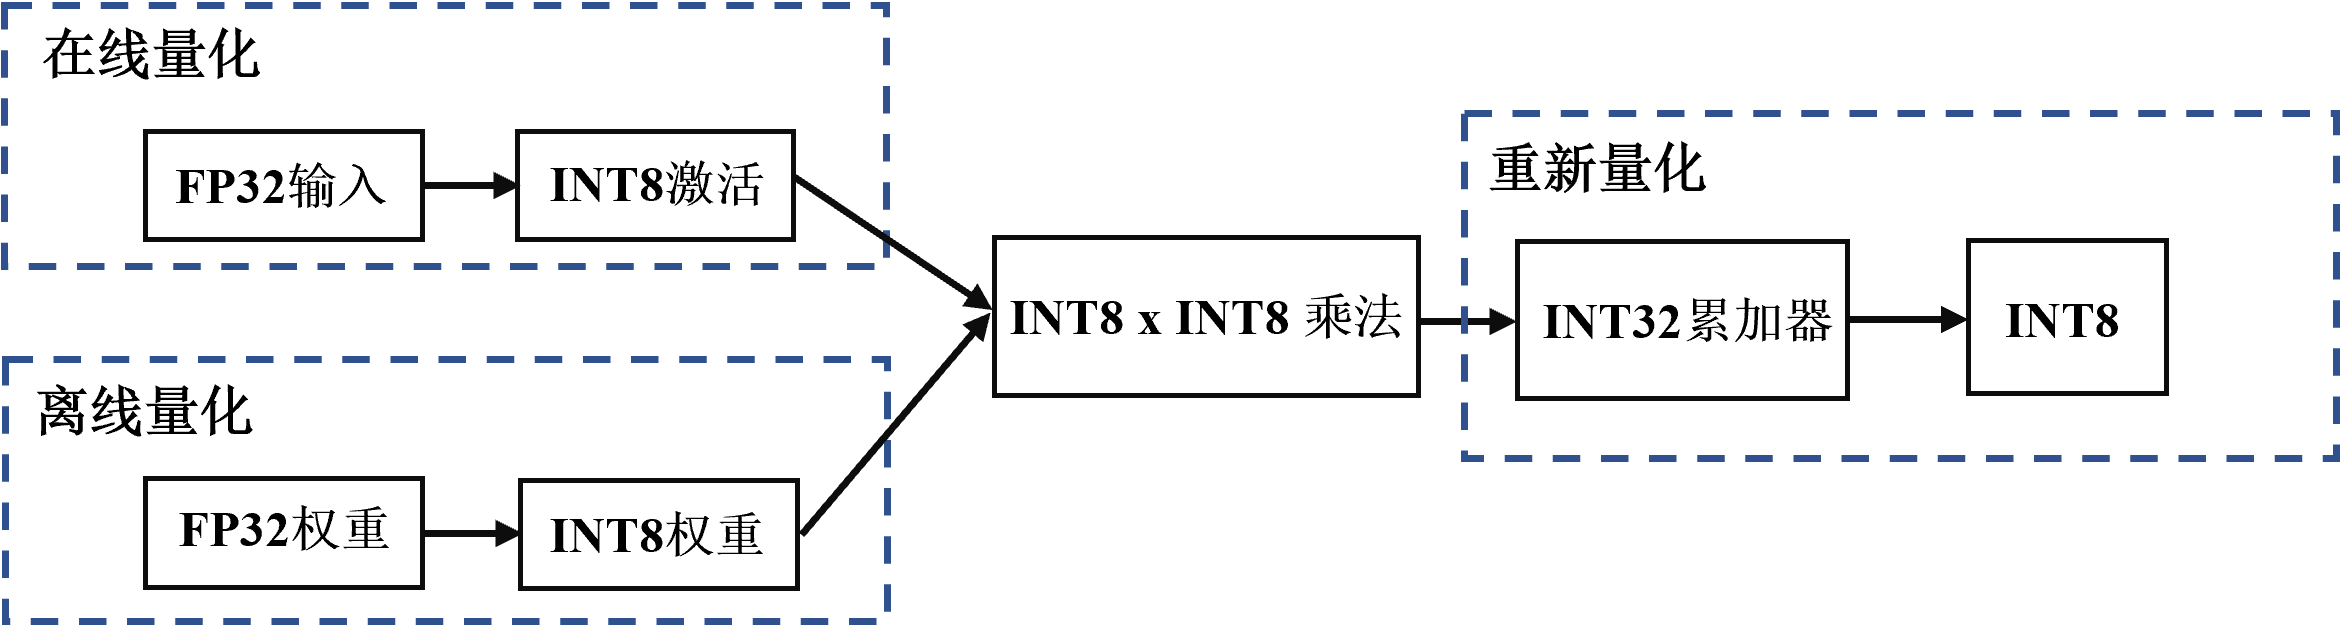
\includegraphics[width=0.82\textwidth]{images/INT8QuantPipine}
  \caption{INT8 量化推理计算流程}
  \label{fig:int8_quant_flow}
\end{figure}

本文从 RT-Pose 训练集中划分 256 组不参与训练的双目样本作为代表性校准集，并保持与部署阶段一致的输入分辨率 $640\times480$ 与 batch=1 预处理流程。校准时，逐层统计骨干卷积与 EFEM 投影/聚合层的激活直方图，枚举候选截断阈值，并以 Kullback-Leibler（KL）散度衡量量化分布与原始分布之间的信息损失；使 KL 散度最小的阈值被选作最终 clip 值，再换算为激活 scale。相较于简单 min-max，该方法对异常大值更稳健，更适合本文中存在长尾响应的跨视图特征张量。算法流程如算法~\ref{alg:ncnn_hist_ptq} 所示。

\begin{algorithm}
  \caption{基于直方图校准的 PTQ 量化算法}
  \label{alg:ncnn_hist_ptq}
  \renewcommand{\algorithmicrequire}{Input:}
  \renewcommand{\algorithmicensure}{Output:}
  \begin{algorithmic}[1]
    \REQUIRE 浮点模型 $\mathcal{M}_{fp}$；代表性校准集 $\mathcal{D}_{cal}$（256 组双目样本）；可量化层集合 $\mathcal{L}_q$；直方图 bin 数 $B$；INT8 量化级数 $Q=128$
    \ENSURE 各层量化参数表 $\mathcal{T}=\{(s_l,c_l)\mid l\in\mathcal{L}_q\}$
    \STATE 根据 4.2.3 节敏感性分析，移除 EFEM scores、热力图/置信度输出与 DWT，得到低敏感可量化层集合 $\mathcal{L}_q$
    \FOR{each $l \in \mathcal{L}_q$}
      \STATE 初始化该层激活统计直方图 $H_l\in\mathbb{R}^{B}$，并置最大绝对值 $a_l^{max}\gets 0$
    \ENDFOR
    \FOR{each 样本 $x \in \mathcal{D}_{cal}$}
      \STATE 将 $x$ 输入浮点模型 $\mathcal{M}_{fp}$，前向计算所有 $l\in\mathcal{L}_q$ 的激活张量 $\mathbf{A}_l(x)$
      \FOR{each $l \in \mathcal{L}_q$}
        \STATE 更新 $a_l^{max}\gets \max(a_l^{max}, \max |\mathbf{A}_l(x)|)$
        \STATE 以区间 $[0,a_l^{max}]$ 为范围，将 $|\mathbf{A}_l(x)|$ 累计到直方图 $H_l$
      \ENDFOR
    \ENDFOR
    \FOR{each $l \in \mathcal{L}_q$}
      \FOR{each 候选截断 bin $t \gets Q,\cdots,B$}
        \STATE 将直方图 $H_l[1:t]$ 压缩为 $Q$ 个量化区间，并把尾部 $H_l[t+1:B]$ 累加到最后一个区间
        \STATE 对压缩后的分布做反量化展开，得到近似分布 $\hat{H}_{l,t}$
        \STATE 计算 KL 散度 $D_{KL}(H_l[1:t]\|\hat{H}_{l,t})$
      \ENDFOR
      \STATE 取 $t^\star=\arg\min_t D_{KL}(H_l[1:t]\|\hat{H}_{l,t})$
      \STATE 计算截断阈值 $c_l=\dfrac{t^\star}{B}a_l^{max}$ 与量化尺度 $s_l=\dfrac{c_l}{Q-1}$
      \STATE 将 $(s_l,c_l)$ 写入量化参数表 $\mathcal{T}$
    \ENDFOR
    \STATE 利用量化参数表 $\mathcal{T}$ 对 MNN 图中对应层执行 INT8 权重/激活量化，并保留豁免层为 FP32
  \end{algorithmic}
\end{algorithm}

该直方图校准方法仅用于低敏感层的 INT8 区间估计，而非对全网络统一量化。根据 4.2.3 节的敏感性结论，EFEM gather/correlation、EFEM softmax 前注意力分数、热力图/置信度输出以及 DWT 求解器在校准前即被移出统计列表，不参与直方图建表。

\begin{table}[htbp]
  \centering
  \small
  \caption{后训练量化关键配置表}
  \label{tab:ptq_config}
  \begin{tabular}{@{}p{0.16\textwidth}p{0.22\textwidth}p{0.46\textwidth}@{}}
    \toprule
    项目 & 设置 & 说明 \\
    \midrule
    导出格式 & ONNX（opset 17） & 输入固定 $[1,3,480,640]$（batch=1） \\
    图优化 & Conv-BN 融合、常量折叠 & 由 \texttt{mnnconvert} 自动完成 \\
    量化对象 & 主体卷积的权重与激活 & 骨干与 EFEM 投影/聚合层参与 INT8 校准 \\
    权重量化 & INT8，per-channel 对称 & 通道尺度更稳健，适配 dotprod \\
    激活量化 & INT8，直方图截断 & 基于直方图/KL 的校准方法 \\
    豁免策略 & 高敏感激活/求解保留 FP32 & EFEM gather/correlation、EFEM scores、热力图/置信度输出、DWT \\
    校准数据 & RT-Pose 代表集 & 仅用于统计分布，不参与参数更新 \\
    校准样本数 & 256 组双目样本 & 从训练集划分，不参与训练，仅用于激活统计 \\
    \bottomrule
  \end{tabular}
\end{table}

\subsection{实验评估}

本节通过三组实验验证所提方案的有效性：首先比较不同精度配置下的精度--效率权衡，其次通过消融实验验证各保护层的必要性，最后考察量化后模型在多人场景中的时延稳定性。

\subsubsection{实验设置}

硬件平台与推理环境。实验在 Xiaomi\,14 真机（Snapdragon 8 Gen3，16\,GB LPDDR5X）上进行，推理框架采用 MNN 2.9.0，启用 ARMv8.2 dotprod 与 FP16 NEON 支持。所有实验均固定 4 线程 CPU 执行环境，预热 10 次后正式计时 100 次，取均值作为延迟报告值；批大小固定为 1，输入分辨率统一为 $640\times480$。

对比配置。本节测试四种精度配置：FP32 全精度、FP16 全精度（第三章基线）、激进 INT8，以及本文混合精度。四种配置共享相同的网络结构、输入尺寸与推理协议，仅精度设置不同。

评估指标。精度以 RT-Pose 验证集上的 MPJPE 均值（mm）衡量，同时记录与 FP16 基线的偏差 $\Delta\text{MPJPE}$；效率以端到端推理延迟（ms，单人场景）和模型文件大小（MB）表征。

\subsubsection{量化方案对比}

四种精度配置的综合评测结果如表~\ref{tab:quant_comparison} 所示。

\begin{table}[htbp]
  \centering
  \small
\caption{不同精度配置的精度与效率对比}
  \label{tab:quant_comparison}
  \begin{tabular}{lcccccc}
    \toprule
    配置 & MPJPE (mm)$\downarrow$ & $\Delta$MPJPE (mm) & 延迟 (ms)$\downarrow$ & 加速比 & 模型大小 (MB) \\
    \midrule
    FP32 全精度               & 158.6 & $\phantom{+}0.0$ & 208.7 & 0.56$\times$ & 46.8 \\
    FP16 全精度（基线）        & 158.6 & $\phantom{+}0.0$ & 116.0 & 1.00$\times$ & 23.4 \\
    激进 INT8                 & 172.0 & $+13.4$          & 67.8  & 1.71$\times$ & 11.7 \\
    本文混合精度               & 160.8 & $\mathbf{+2.2}$ & 72.3 & $\mathbf{1.60\times}$ & 15.2 \\
    \bottomrule
  \end{tabular}
\end{table}

由表~\ref{tab:quant_comparison} 可得到以下结论：

（1）FP32 与 FP16 的 MPJPE 一致，而 FP16 延迟仅为 FP32 的约 56\%，说明本任务在端侧采用 FP16 不会带来可观测精度损失。

（2）激进 INT8 虽取得最高加速比，但 MPJPE 增量达到 $+13.4\,\text{mm}$，说明继续量化高敏感激活会显著破坏跨视图匹配与坐标回归精度。

（3）本文混合精度以 72.3\,ms 的延迟实现 1.60$\times$ 加速，同时仅带来 $+2.2\,\text{mm}$ 的 MPJPE 增量，说明主体卷积的低风险量化已覆盖主要收益来源，而关键保护层有效抑制了额外精度损失。

\subsubsection{消融实验：精度敏感层的必要性验证}

为验证混合精度方案中各精度保护层的必要性，本节以本文方案（表~\ref{tab:precision_allocation}）为基准，逐一将被保护的 FP32 层替换为 INT8，记录 MPJPE 变化。实验结果如表~\ref{tab:ablation_quant} 所示。

\begin{table}[htbp]
  \centering
  \small
\caption{精度敏感层消融实验}
  \label{tab:ablation_quant}
  \begin{tabular}{lccc}
    \toprule
    变体 & MPJPE (mm)$\downarrow$ & $\Delta$MPJPE (mm) & 延迟 (ms) \\
    \midrule
    本文混合精度（基准）                          & 160.8 & $\phantom{+}0.0$ & 72.3 \\
    \quad + EFEM 注意力分数改 INT8               & 167.3 & $+6.5$           & 71.8 \\
    \quad + 热力图/置信度头改 INT8               & 163.5 & $+2.7$           & 72.0 \\
    \quad + DWT 改 INT8（FP32$\to$INT8）        & 168.2 & $+7.4$           & 72.3 \\
    \quad + 以上三者全部改 INT8（$\approx$激进 INT8）& 172.4 & $+11.6$       & 67.8 \\
    \bottomrule
  \end{tabular}
\end{table}

由表~\ref{tab:ablation_quant} 可得到以下结论：

（1）EFEM 注意力分数与 DWT 是最关键的保护层，任一改为 INT8 都会带来约 6--7\,mm 的明显精度退化。

（2）热力图/置信度头改为 INT8 的精度代价相对较小，但其参数量本就很少，继续量化的收益不足以抵消精度损失。

（3）三类保护层同时改为 INT8 后，结果已接近激进 INT8，说明本文所设保护层基本覆盖了主要精度损失来源。

\subsubsection{多人场景量化稳定性分析}

第三章已证明，本文框架的自底向上整图推理链路在人数增加时延迟增长极为平缓（1人 116.0\,ms $\to$ 10人 117.3\,ms）。本节在量化后配置（本文混合精度）下复现该实验，验证 INT8 量化是否影响延迟随人数变化的稳定性。实验结果如表~\ref{tab:multiperson_latency_quant} 所示。

\begin{table}[htbp]
  \centering
  \small
\caption{量化前后多人场景延迟对比}
  \label{tab:multiperson_latency_quant}
  \begin{tabular}{cccc}
    \toprule
    人数 $M$ & FP16 基线 (ms) & 混合 INT8 (ms) & 加速比 \\
    \midrule
     1 & 116.0 & 72.3 & 1.60$\times$ \\
     2 & 116.0 & 72.3 & 1.60$\times$ \\
     3 & 116.1 & 72.4 & 1.60$\times$ \\
     5 & 116.3 & 72.5 & 1.60$\times$ \\
     7 & 116.5 & 72.8 & 1.60$\times$ \\
    10 & 117.3 & 73.4 & 1.60$\times$ \\
    \bottomrule
  \end{tabular}
\end{table}

量化前后，随人数增加的延迟增长模式基本一致（$\Delta$延迟 $\leq 1.3\,\text{ms}$），且各人数配置下的加速比稳定保持在 1.60$\times$。这说明本文量化方案并未改变自底向上整图推理的时延特性，多人场景下的额外开销仍主要来自后处理阶段，而非量化本身。该结果说明，本文方案不仅在单人场景下有效，也具备面向多人动态场景的部署稳定性。

\subsection{本章小结}

本章围绕 Snapdragon 8 Gen3 CPU 端侧部署场景，完成了从性能瓶颈识别到混合精度落地验证的闭环分析，可归纳为以下三点。

第一，端到端时延的主要瓶颈集中在双分支骨干卷积，而 EFEM gather 虽计算量有限，却因不规则访存成为额外热点。Roofline 分析进一步表明，骨干主要受算力约束，EFEM 投影、头部卷积与 gather 更接近带宽约束，因此 INT8 在本文模型上的收益来源同时包含算力侧加速与访存侧压缩。

第二，量化风险在网络中呈明显非均匀分布。骨干权重与 EFEM 投影权重属于低风险高收益量化对象，而 EFEM gather/correlation、EFEM 注意力分数、热力图/置信度输出以及 DWT 求解器直接影响访存瓶颈收益实现、匹配分布与几何求解稳定性，应作为保护层保留 FP32。基于这一结论，本文形成了“瓶颈定位 + 敏感性筛查 + 分层混合精度设计”的硬件感知量化方法链。

第三，实验结果验证了该方案在目标平台上的有效性。本文混合精度方案以 $+2.2\,\text{mm}$ 的 MPJPE 代价实现 1.60$\times$ 推理加速，并将模型体积由 23.4\,MB 压缩至 15.2\,MB；相较于激进 INT8，保留了主要加速收益，同时显著降低了精度退化。多人场景实验进一步表明，量化后模型仍保持与第三章基线一致的时延增长规律。

因此，本章的贡献不在于给出某一组固定平台参数下的经验配置，而在于形成了一套可迁移的硬件感知量化分析路径：先定位瓶颈，再识别敏感层，最后设计分层混合精度与 PTQ 校准流程。上述结论针对 Snapdragon 8 Gen3 CPU 与 MNN 推理后端这一特定执行环境成立；当迁移到其他 SoC、GPU/NPU 后端或不同推理框架时，仍需结合目标平台重新标定瓶颈位置与敏感层集合，但本文给出的“瓶颈定位 + 敏感性筛查 + 分层混合精度设计”方法链具有可复用的方法论价值。

\section{总结与展望}

本文面向移动端多人三维人体姿态估计任务，围绕双目视觉模型在端侧部署中存在的计算冗余大、跨视图交互开销高以及压缩部署困难等问题，系统开展了轻量化网络设计与硬件感知部署优化研究。全文以双目几何约束、轻量化模型构建和混合精度量化部署为主线，逐步完成了从方法设计、实验验证到真实设备落地的研究闭环。

\subsection{总结}

本文的主要研究工作和结论可概括如下。

第一，本文围绕移动端双目三维人体姿态估计的应用需求和技术挑战，系统分析了三维人体姿态估计、双目几何约束、轻量化网络设计以及模型压缩部署等相关研究进展，明确了本文的核心问题，即如何在资源受限设备上兼顾三维估计精度、推理时延与模型体积，为后续研究内容奠定了理论基础。

第二，针对传统双目方法中左右分支对称建模导致的冗余计算，以及稠密立体匹配链路不利于端侧实时部署的问题，本文提出了轻量化非对称双目三维人体姿态估计框架。该框架以“左重右轻”的非对称双分支骨干为基础，通过极线特征增强模块在一维视差窗口内完成跨视图几何信息交互，并结合可微加权三角化求解器实现端到端三维姿态恢复；同时引入跨分支一致性约束以减小轻量分支与全量分支之间的表征差异。实验结果表明，所提方法在保持较低参数量和 FLOPs 的同时，能够获得较好的三维姿态估计精度，并具备适合多人场景整图推理的稳定时延特性。

第三，针对移动端 CPU 平台下“哪些模块适合量化、哪些模块需要保护”的部署问题，本文提出了硬件感知的混合精度量化方案。通过端到端延迟拆解、Roofline 瓶颈分析和量化敏感性筛查，识别出骨干主体卷积是量化加速的主要收益来源，而 EFEM 注意力分数、热力图/置信度输出以及 DWT 求解链路则属于高敏感模块。在此基础上，本文设计了分层混合精度策略，并采用基于直方图校准的 PTQ 方法完成 MNN 部署。实验结果表明，所提方案在 Xiaomi 14 平台上以较小的 MPJPE 增量实现了显著的推理加速与模型压缩，验证了“瓶颈定位 + 敏感性筛查 + 分层混合精度设计”方法链在真实移动端场景中的有效性。

总体而言，本文工作的意义主要体现在两个方面：一是从模型设计角度提出了适合移动端双目多人三维姿态估计的轻量化网络结构，降低了传统双目方法对对称大骨干和稠密代价体的依赖；二是从部署优化角度形成了面向目标平台的硬件感知量化分析与落地方法，为后续同类端侧视觉模型的压缩部署提供了可借鉴的研究思路。

\subsection{展望}

尽管本文在轻量化双目三维人体姿态估计与移动端混合精度部署方面取得了一定进展，但仍存在有待进一步完善之处，未来可从以下几个方向继续开展研究。

第一，本文当前的部署验证主要基于 Snapdragon 8 Gen3 CPU 与 MNN 推理后端展开，所得瓶颈结论和精度分配策略仍具有一定的平台相关性。未来可进一步面向 GPU、NPU 以及不同 SoC 平台开展跨硬件对比研究，结合不同算子支持特性、存储层次和调度机制，探索更具通用性的硬件协同设计方法。

第二，本文提出的轻量化双目框架已有效降低跨视图交互开销，但在极端遮挡、远距离小目标以及复杂多人交互场景下，跨视图匹配与三维恢复仍有进一步提升空间。后续可结合更强的几何先验建模、时序信息利用或多模态传感信息融合，以增强模型在复杂动态环境下的鲁棒性与泛化能力。

第三，本文在量化部署中采用了基于代表集校准的 PTQ 方法，并对高敏感模块保留 FP32 保护路径。该策略在工程上较为稳妥，但仍未充分挖掘量化训练与端侧算子协同优化的潜力。未来可进一步研究面向双目三维姿态估计任务的量化感知训练、低比特激活建模以及更细粒度的混合精度分配策略，以在保持数值稳定性的同时继续提升部署效率。

第四，本文当前实验主要集中在 RT-Pose 等真实场景数据上的模型精度与时延评估，对于长期运行稳定性、端侧功耗控制以及不同光照和相机参数变化下的系统鲁棒性仍有待进一步验证。未来可面向更丰富的实际应用场景开展系统级实验，推动所提方法从论文验证进一步走向工程化落地。

综上所述，本文围绕移动端多人三维人体姿态估计任务完成了从模型设计到端侧部署的较完整研究。随着移动端异构计算能力的持续提升以及实时三维感知需求的不断增长，轻量化、高精度、可部署的三维人体姿态估计方法仍具有重要的研究价值。本文的工作可视为该方向的一次阶段性探索，并可为后续相关研究提供基础与参考。

% \input{content/format_examples.tex}
